%!TEX TS-program = pdflatex
% dissertation.tex -- main dissertation file
%
% Wisconsin dissertation template
% Copyright (c) 2008-2009 William C. Benton.  All rights reserved.
%
% This program can redistributed and/or modified under the terms
% of the LaTeX Project Public License Distributed from CTAN
% archives in directory macros/latex/base/lppl.txt; either
% version 1 of the License, or (at your option) any later version.
%
% This program includes other software that is licensed under the
% terms of the LPPL and the Perl Artistic License; see README for details.
%
% You, the user, still hold the copyright to any document you produce
% with this software (like your dissertation).
%

%%% You'll want ``oneside'' for the deposit version, but probably not for any versions that don't need to meet the UW requirements
%\documentclass[12pt,letterpaper]{memoir}
\documentclass[12pt,oneside,letterpaper]{memoir}

% preamble.tex -- packages to include
%
% Wisconsin dissertation template
% Copyright (c) 2008 William C. Benton.  All rights reserved.
%
% This program can redistributed and/or modified under the terms
% of the LaTeX Project Public License Distributed from CTAN
% archives in directory macros/latex/base/lppl.txt; either
% version 1 of the License, or (at your option) any later version.
%
% This program includes other software that is licensed under the
% terms of the LPPL and the Perl Artistic License; see README for details.
%
% You, the user, still hold the copyright to any document you produce
% with this software (like your dissertation).

%% You should use natbib
\IfFileExists{natbib.sty}{%
\usepackage{natbib}%
}{}

%% You probably need appendix, if you want appendices
\IfFileExists{appendix.sty}{%
\usepackage{appendix}%
}{}

%% the spacing in memoir is weird, you'll need to use this
\DisemulatePackage{setspace}
%\usepackage[doublespacing]{setspace}
\usepackage[onehalfspacing]{setspace}

%% geometry package to help with margins on title page
\usepackage{geometry}

%% List setup; the ``hanglist`` environment will allow you to have
%% nicely-typeset enumerated lists (i.e. with the numbers hanging in
%% the margins).  You need at least version 2.1 of enumitem.sty.  If
%% you don't have enumitem installed at all, hanglist will just be an
%% alias for enumerate.
\IfFileExists{enumitem.sty}{%
\usepackage[loadonly]{enumitem}[2007/06/30]%
\newlist{hanglist}{enumerate}{1}% 
\setlist[hanglist]{label=\arabic*.}%
\setlist[hanglist,1]{leftmargin=0pt}%
}{%
\newenvironment{hanglist}{\begin{enumerate}}{\end{enumerate}}%
}

%% Comment out any of these that you don't want
\usepackage{amssymb}
\usepackage{amsmath}
\usepackage{amsthm}
%\usepackage{theorem}
\usepackage[linktocpage=true]{hyperref} %for clickable links in toc

%\IfFileExists{mathpartir.sty}{%
%\usepackage{mathpartir}%
%}{}

%%%%% LISTINGS package and setup
\IfFileExists{listings.sty}{%
\usepackage{listings}%
}{}



%% Get rid of ugly borders around PDF hyperlinks (e.g. for cross-references, bib entries, or URLs)
\hypersetup{pdfborder = 0 0 0}

%% You want microtype.
\IfFileExists{microtype.sty}{%
\usepackage[protrusion=true,expansion=true]{microtype}%
}{}

%\pagestyle{thesisdraft}

% Surround parts of graphics with box
\usepackage{boxedminipage}

%% booktabs (thx to Nate Rosenblum for bringing this beautiful package
%% to my attention)
\IfFileExists{booktabs.sty}{%
\usepackage{booktabs}%
}{}

% This is now the recommended way for checking for PDFLaTeX:
\usepackage{ifpdf}

%% Avoid ugly "Type 3" fonts
\usepackage{lmodern}
\usepackage[LY1]{fontenc}


%% Substitute your favorite serif and sans fonts here....
\IfFileExists{tgcursor.sty}{%
% TeX Gyre pagella, like Palatino
\usepackage{tgcursor}%
}{}

%\usepackage[LY1]{eulervm}

\ifpdf
\usepackage[pdftex]{graphicx}
\else
\usepackage{graphicx}
\fi

\usepackage{makeidx}
\makeindex

{\theoremstyle{plain}
\newtheorem{thm}{Theorem}[chapter]
\newtheorem{cor}[thm]{Corollary}
\newtheorem{define}[thm]{Definition}
\newtheorem{exmpl}[thm]{Example}
}
{\theoremstyle{remark}
\newtheorem{rmk}[thm]{Remark}
}

\newtheoremstyle{customsty1}
{3pt}%
{3pt}%
{}% --- body font
{}% --- indent amount
{\bfseries}% --- Theorem head font
{:}% --- Punctuation after head
{.5em}% --- space after head
{}% --- theorem head spec (can be left empty, meaning 'normal')

% Define 'newtheorems' that use ``customsty1''
{\theoremstyle{customsty1} 
}


%%% NB: the ``deposit'' chapter- and page- styles should conform to UW
%%% requirements.  If you are producing a pretty version of your
%%% dissertation for web use later, you will certainly want to make
%%% your own chapter and page styles.

\makechapterstyle{deposit}{%
  \renewcommand{\chapterheadstart}{}
  \renewcommand{\printchaptername}{}
  \renewcommand{\chapternamenum}{}
  \renewcommand{\printchapternum}{\parbox{2em}{\MakeLowercase{\Huge\scshape\thechapter{}}} }
  %\renewcommand{\printchapternum}{\parbox{2em}{\MakeLowercase{\Large\scshape\thechapter{}}} }
  \renewcommand{\afterchapternum}{}
  \renewcommand{\printchaptertitle}[1]{%
  \raggedright\Huge\scshape\MakeLowercase{##1}}
  %\raggedright\Large\scshape\MakeLowercase{##1}}
  \renewcommand{\afterchaptertitle}{%
  \vskip\onelineskip \hrule\vskip\onelineskip}
}

\makepagestyle{deposit}
 
\makeatletter
 
\renewcommand{\chaptermark}[1]{\markboth{#1}{}}
\renewcommand{\sectionmark}[1]{\markboth{#1}{}}
 
\makeevenfoot{deposit}{}{}{}
\makeoddfoot{deposit}{}{}{}
\makeevenhead{deposit}{\thepage}{}{}
\makeoddhead{deposit}{}{}{\thepage}
\makeatother

%%% set up page numbering for chapter pages to satisfy UW requirements
%%% NB: You will want to delete until the ``SNIP'' mark if you are
%%% making a ``nice'' copy
\copypagestyle{chapter}{plain}
\makeoddfoot{chapter}{}{}{}
\makeevenhead{chapter}{\thepage}{}{}
\makeoddhead{chapter}{}{}{\thepage}
%%% SNIP

%%% bib nonsense
\makeatletter
\newenvironment{wb-bib}[1]{%
  \chapter*{references}
\ifnobibintoc\else 
\phantomsection 
\addcontentsline{toc}{chapter}{References} 
\fi 
\prebibhook
  \begin{bibitemlist}{#1}}{\end{bibitemlist}\postbibhook}

\AtBeginDocument{%
  \@ifpackageloaded{natbib}{% natbib is loaded
    \addtodef{\endthebibliography}{}{\vskip-\lastskip\postbibhook}
    \@ifpackagewith{natbib}{sectionbib}{% with sectionbib option
      \renewcommand{\bibsection}{\@memb@bsec}}%
      {\renewcommand{\bibsection}{\@memb@bchap}}}%
  {}
  \@ifpackagewith{chapterbib}{sectionbib}{%
    \renewcommand{\sectionbib}[2]{}
    \renewcommand{\bibsection}{\@memb@bsec}}{}
}
\makeatother

% defs.tex -- wbepi environment for chapter epigraphs and other useful defs.
%
% Wisconsin dissertation template
% Copyright (c) 2008 William C. Benton.  All rights reserved.
%
% This program can redistributed and/or modified under the terms
% of the LaTeX Project Public License Distributed from CTAN
% archives in directory macros/latex/base/lppl.txt; either
% version 1 of the License, or (at your option) any later version.
%
% This program includes other software that is licensed under the
% terms of the LPPL and the Perl Artistic License; see README for details.
%
% You, the user, still hold the copyright to any document you produce
% with this software (like your dissertation).


%% put lstnewenvironment declarations here, if you're using listings

%% end lstnewenvironment declarations

%% I put convenience definitions that will go in several chapters here

%%%%% begin convenience definitions
\usepackage{multirow} % multirow in tables
\usepackage{rotating} % rotatebox in tables
\usepackage{commath} % abs
\usepackage{xfrac} % sfrac

\usepackage{xspace} % space in command definitions

% for mathscr
\usepackage{mathrsfs}
%\usepackage{unicode-math}
%\setmathfont{XITS Math}
%\setmathfont[version=setB,StylisticSet=1]{XITS Math}

% center table not caption
\usepackage[justification=justified,margin=15pt,labelfont=bf,font=sl,format=hang,indention=-1.5cm]{caption}



% units
\newcommand{\keV}{\ensuremath{\mathrm{keV}}\xspace}
\newcommand{\MeV}{\ensuremath{\mathrm{MeV}}\xspace}
\newcommand{\GeV}{\ensuremath{\mathrm{GeV}}\xspace}
\newcommand{\TeV}{\ensuremath{\mathrm{TeV}}\xspace}
\newcommand{\fbinv}{\ensuremath{\mathrm{fb}^{-1}}\xspace}
\newcommand{\fb}{\ensuremath{\mathrm{fb}}\xspace}
\newcommand{\ns}{\ensuremath{\mathrm{ns}}\xspace}
\newcommand{\lumi}{\ensuremath{\mathcal L}\xspace}
\newcommand{\tlumi}{\ensuremath{\int\mathcal{L} dt}\xspace}
\newcommand{\dldt}{\ensuremath{d\mathcal L/dt}\xspace}

\newcommand{\pbw}{\ensuremath{\mathrm{PbWO}_4}\xspace}

% kinematics
\newcommand{\pt}{\ensuremath{p_T}\xspace}
\newcommand{\mt}{\ensuremath{m_T}\xspace}
\newcommand{\et}{\ensuremath{E_T}\xspace}
\newcommand{\etg}{\ensuremath{E_T^\gamma}\xspace}
\newcommand{\ptg}{\ensuremath{p_T^\gamma}\xspace}
\newcommand{\vmet}{\ensuremath{E_T^{\mathrm{miss}}}\xspace}
\newcommand{\met}{\ensuremath{E_T^{\mathrm{miss}}}\xspace}
\newcommand{\s}{\ensuremath{\sqrt{s}=}\xspace}

% generators
%\newcommand{\MCFM}{{\tt MCFM}\xspace}
%\newcommand{\GEANT}{{\tt GEANT}\xspace}
%\newcommand{\FEWZ}{{\tt FEWZ}\xspace}
%\newcommand{\CTEQ}{{\tt CTEQ}\xspace}
%\newcommand{\MSTW}{{\tt MSTW}\xspace}
%\newcommand{\NNPDF}{{\tt NNPDF}\xspace}
%\newcommand{\HERA}{{\tt HERA}\xspace}
%\newcommand{\QUETP}{{\tt QUETP}\xspace}
%\newcommand{\MADGRAPH}{{\tt MADGRAPH}\xspace}
%\newcommand{\PYTHIA}{{\tt PYTHIA}\xspace}
%\newcommand{\PYTHIAs}{{\tt PYTHIA6}\xspace}
%\newcommand{\PYTHIAe}{{\tt PYTHIA8}\xspace}

\newcommand{\MCFM}{{MCFM}\xspace}
\newcommand{\GEANT}{{GEANT}\xspace}
\newcommand{\FEWZ}{{FEWZ}\xspace}
\newcommand{\CTEQ}{{CTEQ}\xspace}
\newcommand{\MSTW}{{MSTW}\xspace}
\newcommand{\NNPDF}{{NNPDF}\xspace}
\newcommand{\HERA}{{HERA}\xspace}
\newcommand{\QUETP}{{QUETP}\xspace}
\newcommand{\MADGRAPH}{{MADGRAPH}\xspace}
\newcommand{\PYTHIA}{{PYTHIA}\xspace}
\newcommand{\PYTHIAs}{{PYTHIA6}\xspace}
\newcommand{\PYTHIAe}{{PYTHIA8}\xspace}
%\newcommand{\abs}{\ensuremath{absFIXME}\xspace}

% wbb
\newcommand{\wbb}{\ensuremath{\w b\bar{b}}\xspace}
\newcommand{\bbbar}{\ensuremath{b\bar{b}}\xspace}
\newcommand{\ppwbblnbb}{\ensuremath{pp\rightarrow Wb\bar{b}\rightarrow\ell\nu b\bar{b}}\xspace}
\newcommand{\ppwbb}{\ensuremath{pp\rightarrow Wb\bar{b}}\xspace}
\newcommand{\w}{\ensuremath{\mathrm{W}}\xspace}
%\newcommand{\v}{\ensuremath{\mathrm{V}}\xspace}
\newcommand{\z}{\ensuremath{\mathrm{Z}}\xspace}

% samples
\newcommand{\vjets}{\ensuremath{\mathrm{V}+\mathrm{jets}}\xspace}
\newcommand{\wjets}{\ensuremath{\w+\mathrm{jets}}\xspace}
\newcommand{\wcc}{\ensuremath{\w c\bar{c}}\xspace}
\newcommand{\wc}{\ensuremath{\w c}\xspace}
\newcommand{\wudscg}{\ensuremath{\w usdcg}\xspace}
\newcommand{\gjets}{\ensuremath{\gamma+\mathrm{jets}}\xspace}
\newcommand{\zll}{\ensuremath{Z\ell\bar{\ell}}\xspace}
\newcommand{\zjj}{\ensuremath{\z jj}\xspace}
\newcommand{\zbb}{\ensuremath{\z \bbbar}\xspace}
\newcommand{\WW}{\ensuremath{\w\w}\xspace}
\newcommand{\WZ}{\ensuremath{\w\z}\xspace}
\newcommand{\ZZ}{\ensuremath{\z\z}\xspace}
\newcommand{\ttbar}{\ensuremath{t\bar{t}}\xspace}



% monophoton
\newcommand{\gmet}{\ensuremath{\gamma+\met}\xspace}
\newcommand{\zee}{\ensuremath{\z\rightarrow e\bar{e}}\xspace}
\newcommand{\ttg}{\ensuremath{t\bar{t}\gamma}\xspace}
\newcommand{\wen}{\ensuremath{\w\rightarrow e\nu}\xspace}
\newcommand{\wmn}{\ensuremath{\w\rightarrow \mu\nu}\xspace}
\newcommand{\ppzgnng}{\ensuremath{pp\rightarrow \z\gamma\rightarrow\nu\bar{\nu}\gamma}\xspace}
\newcommand{\ppzg}{\ensuremath{pp\rightarrow \z\gamma}\xspace}
\newcommand{\zgnng}{\ensuremath{\z\gamma\rightarrow\nu\bar{\nu}\gamma}\xspace}
\newcommand{\zgllg}{\ensuremath{\z\gamma\rightarrow\ell\bar{\ell}\gamma}\xspace}
\newcommand{\zllg}{\ensuremath{\z\rightarrow\ell\bar{\ell}\gamma}\xspace}
\newcommand{\znn}{\ensuremath{\z\rightarrow\nu\bar{\nu}}\xspace}
\newcommand{\vg}{\ensuremath{V\gamma}\xspace}
\newcommand{\zg}{\ensuremath{\z\gamma}\xspace}
\newcommand{\wg}{\ensuremath{\w\gamma}\xspace}
\newcommand{\sieie}{\ensuremath{\sigma_{i\eta i\eta}}\xspace}
\newcommand{\sieip}{\ensuremath{\sigma_{i\eta i\phi}}\xspace}
\newcommand{\sipip}{\ensuremath{\sigma_{i\phi i\phi}}\xspace}
\newcommand{\DphiMETg}{\ensuremath{\Delta \phi(\met, \gamma)}\xspace}
\newcommand{\DphiMETj}{\ensuremath{\Delta \phi(\vmet, j)}\xspace}
\newcommand{\minDphiMETj}{\ensuremath{\mathrm{min}\DphiMETj}\xspace}



\newcommand{\wglng}{\ensuremath{\w\gamma\rightarrow \ell\nu\gamma}\xspace}
\newcommand{\wlng}{\ensuremath{\w\rightarrow \ell\nu\gamma}\xspace}
\newcommand{\sigetaeta}{\ensuremath{\sigma_{\eta\eta}}\xspace}
\newcommand{\as}{\ensuremath{\alpha_s}\xspace}
\newcommand{\MGfiveAMC} {\textsc{MadGraph5\_aMC@NLO}\xspace}
\newcommand{\NNPDFthree}{\textsc{NNPDF3.0}\xspace}
\newcommand{\DYRes}{\textsc{DYRes}\xspace}


\makeatletter
\newcommand{\wb@episource}{}
\newenvironment{wbepi}[1]{\begin{quote}\renewcommand{\wb@episource}{#1}\itshape}{\par\upshape \raggedleft --- \textsc{\wb@episource}\\ \end{quote}}
\makeatother

%%%%% SVN
\IfFileExists{svn-multi.sty}{%
\usepackage{svn-multi}%
%%% Uncomment the second one and comment out the first one if you want
%%% to include subversion revision information in each file.
\newcommand{\vcinfo}{}%
%\newcommand{\vcinfo}{\begin{centering}\fbox{\fbox{\parbox{5in}{Author: \svnauthor\\Revision: \svnfilerev\\Last changed on: \svnfiledate\\URL: \svnkw{HeadURL}}}}\\[1em]\end{centering}}%
}{%
\newcommand{\svnidlong}[4]{}%
\newcommand{\svnfilerev}{}%
\newcommand{\svnauthor}{}%
\newcommand{\svnfiledate}{}%
\newcommand{\svnkw}{}%
\newcommand{\vcinfo}{}%
}

%%%%% end convenience definitions

% thesisdefs.tex

% This is mostly adapted from withesis.cls.  The original copyright
% notice for withesis.cls follows, preceded by two percent signs (%%):

%% withesis.cls
%% LaTeX Style file for the University of Wisconsin-Madison Thesis Format
%% Adapted from the Purdue University Thesis Format
%% Originally by Dave Kraynie
%% Edits by Darrell McCauley
%% Adapted to UW-Madison format by Eric Benedict  (Noted with <EB>)
%% Updated to LaTeX2e by Eric Benedict 24 July 00
%% 
%%=============================================================================
%% Licensed under the Perl Artistic License.
%% see: http://www.ctan.org/tex-archive/help/Catalogue/licenses.artistic.html
%% for more info...
%%=============================================================================

% withesis.cls is available from CTAN.  The modifications to this file
% are also licensed under the Perl Artistic License.

% --wb, 2008

\makeatletter

\newcounter {tocpage}
\newcounter {lofpage}
\newcounter {lotpage}
\newcounter {listofheading}

\newcommand\@thesistitlemedskip{0.25in}
\newcommand\@thesistitlebigskip{0.55in}
\newcommand{\degree}[1]{\gdef\@degree{#1}}
\newcommand{\project}{\gdef\@doctype{A masters project report}}
\newcommand{\prelim}{\gdef\@doctype{A preliminary report}}
\newcommand{\thesis}{\gdef\@doctype{A thesis}}
\newcommand{\dissertation}{\gdef\@doctype{A dissertation}}
\newcommand{\department}[1]{\gdef\@department{(#1)}}
\newcommand{\oralexamdate}[1]{\gdef\@oralexamdate{#1}} 
\newcommand{\committeeone}[1]{\gdef\@committeeone{#1}}
\newcommand{\committeetwo}[1]{\gdef\@committeetwo{#1}}
\newcommand{\committeethree}[1]{\gdef\@committeethree{#1}}
\newcommand{\committeefour}[1]{\gdef\@committeefour{#1}}
\newcommand{\committeefive}[1]{\gdef\@committeefive{#1}}
\newcommand{\committeesix}[1]{\gdef\@committeesix{#1}}
\newcommand{\committeeseven}[1]{\gdef\@committeeseven{#1}}

\newenvironment{titlepage}
 {\@restonecolfalse\if@twocolumn\@restonecoltrue\onecolumn
  \else \newpage \fi \thispagestyle{empty}
% \c@page\z@ -- deleted: count title page in thesis
}{\if@restonecol\twocolumn \else \newpage \fi}

\gdef\@degree{Doctor of Philosophy}    %Default is PhD
\gdef\@doctype{A dissertation}         %Default is dissertation

\gdef\@department{(Electrical Engineering)} % Default is Electical Engineering
\gdef\@oralexamdate{}
\gdef\@committeeone{}
\gdef\@committeetwo{}
\gdef\@committeethree{}
\gdef\@committeefour{}
\gdef\@committeefive{}
\gdef\@committeesix{}
\gdef\@committeeseven{}



\renewcommand{\maketitle}{%
  \begin{titlepage}
%-----------------------------------------------------------------------------
% -- The thesis office doesn't like thanks on title page.  Put it in
% -- the acknowledgments.  This is here so you don't have to change
% -- your titlepage when converting from report style. -> from Purdue, but I
%        left it here since it seems compatible with UW-Madison, Eric
%-----------------------------------------------------------------------------
    \def\thanks##1{\typeout{Warning: `thanks' deleted from thesis titlepage.}}
    \let\footnotesize\small \let\footnoterule\relax \setcounter{page}{1}
 %sets new margins for title page so that committee members can be placed there

   % \vspace*{0.1in}
    \begin{center}
      %{\textbf{\expandafter\uppercase\expandafter{\@title}}} \\[\@thesistitlebigskip]
      {\textbf{\expandafter\expandafter{\@title}}} \\[\@thesistitlebigskip]
       by \\[\@thesistitlemedskip]
      \@author \\[\@thesistitlebigskip]
      \@doctype\ submitted in partial fulfillment of \\
      the requirements for the degree of\\[\@thesistitlebigskip]
      \@degree \\[\@thesistitlemedskip]
      \@department \\[\@thesistitlebigskip]
      at the \\[\@thesistitlebigskip]
      UNIVERSITY OF WISCONSIN--MADISON\\[\@thesistitlebigskip]
      \@date \\[\@thesistitlebigskip]
    \end{center}
% section added by Steven Baumgart on 3/2012
% adds committee list to the title page
% add or delete committee members as you need to, these are defined in the dissertation.tex document 
% comment out other things as you need to as well. - SB

\noindent Date of final oral examination: \@oralexamdate \hspace*{\fill} \\[\@thesistitlemedskip]
\noindent The dissertation is approved by the following members of the Final Oral Committee:\\*
\indent \@committeeone\\*
\indent \@committeetwo\\*
\indent \@committeethree\\*
\indent \@committeefour\\*
\indent \@committeefive
%\indent \@committeesix\\* %if you uncomment any of these you the last line needs to have no line break ``//*``
%\indent \@committeeseven


  \end{titlepage}

  \setcounter{footnote}{0}
  \setcounter{page}{1} %title page is NOT counted
  \let\thanks\relax
  \let\maketitle\relax \let\degree\relax \let\project\relax \let\prelim\relax
  \let\department\relax
  \gdef\@thanks{}\gdef\@degree{}\gdef\@doctype{}
  \gdef\@department{}
  %\gdef\@author{}\gdef\@title{}
}


%=============================================================================
% ABSTRACT
%=============================================================================
% The abstract should begin with two single-spaced lines describing
% the author and title in a standard format.  After these lines comes
% the standard abstract.
%=============================================================================
\def\abstract{
  \chapter*{Abstract}
  \addcontentsline{toc}{chapter}{Abstract}
  \relax\markboth{Abstract}{Abstract}}
\def\endabstract{\par\newpage}


%=============================================================================
% UMI ABSTRACT
%=============================================================================
% The UMI abstract should begin with the author and title in a standard format.
% After the author comes the advisor and university. After these lines comes
% a bunch of double spaced text to make up the standard abstract.
% After the abstract, the advisor's approval signature follows.
% This page is not numbered and is delivered seperately to the thesis office.
%=============================================================================

\def\advisortitle#1{\gdef\@advisortitle{#1}}
\def\advisorname#1{\gdef\@advisorname{#1}}
\gdef\@advisortitle{Professor}
\gdef\@advisorname{Cheer E.\ Place}

\def\umiabstract{
             \thispagestyle{empty}
                  \addtocounter{page}{-1}
                \begin{center}
                  {\textbf{\expandafter\uppercase\expandafter{\@title}}}\\
                  \vspace{12pt}
                  \@author \\
                  \vspace{12pt}
                  Under the supervision of \@advisortitle\ \@advisorname\\
                  At the University of Wisconsin-Madison
                \end{center}
}

\def\endumiabstract{\vfill \hfill\@advisorname\par\newpage}


%============================================================================
% VERBATIMFILE
%============================================================================
% \verbatimfile{<filename>}    for verbatim inclusion of a file
% - Note that the precise layout of line breaks in this file is important!
% - added the \singlespace - EB
%============================================================================
\def\verbatimfile#1{\begingroup \singlespace
                    \@verbatim \frenchspacing \@vobeyspaces
                    \input#1 \endgroup
}


%=============================================================================
% SEPARATOR Pages
%   Creates a blank page with a text centered horizontally and vertically.
%   The page is neither counted nor numbered.
%   These pages are required in the thesis format before sections such
%   as appendices, vita, bibliography, etc.
%=============================================================================
\def\separatorpage#1{
  \newpage
  \thispagestyle{empty}
  \addtocounter{page}{-1}
  \null
  \vfil\vfil
  \begin{center}
    {\textbf{#1}}
  \end{center}
  \vfil\vfil
  \newpage}


%=============================================================================
% COPYRIGHTPAGE
%=============================================================================
% The copyright must do the following:
% - start a new page with no number
% - place the copyright text centered at the bottom.
%=============================================================================
\def\copyrightpage{
  \newpage
  \thispagestyle{empty}    % No page number
  \addtocounter{page}{-1}
  \chapter*{}            % Required for \vfill to work
  \begin{center}
   \vfill
   \copyright\ Copyright by \@author\ \@date\\
   All Rights Reserved
  \end{center}}


%=============================================================================
% GLOSSARY
%=============================================================================
% The glossary environment must do the following:
% - produce the table of contents entry for the glossary
% - start a new page with GLOSSARY centered two inches from the top
%=============================================================================
\def\glossary{
  \chapter*{GLOSSARY}
  \addcontentsline{toc}{chapter}{Glossary}}
\def\endglossary{\par\newpage}

%=============================================================================
% NOMENCLATURE
%=============================================================================
% The nomenclature environment must do the following:
% - produce the table of contents entry for the nomenclature section
% - start a new page with NOMENCLATURE centered two inches from the top
%=============================================================================
\def\nomenclature{\separatorpage{DISCARD THIS PAGE}
  \chapter*{Nomenclature}
  \addcontentsline{toc}{chapter}{NOMENCLATURE}}
\def\endnomenclature{\par\newpage}

%=============================================================================
% CONVENTIONS
%=============================================================================
% The conventions environment must do the following:
% - produce the table of contents entry for the nomenclature section
% - start a new page with CONVENTIONS centered two inches from the top
%=============================================================================
\def\conventions{\separatorpage{DISCARD THIS PAGE}
  \chapter*{Conventions}
  \addcontentsline{toc}{chapter}{CONVENTIONS}}
\def\endconventions{\par\newpage}


%=============================================================================
% COLOPHON
%=============================================================================
% The colophon environment must do the following:
% - produce the table of contents entry for the nomenclature section
% - start a new page with COLOPHON centered two inches from the top
%=============================================================================
\def\colophon{\separatorpage{DISCARD THIS PAGE}
  \chapter*{Colophon}
  \addcontentsline{toc}{chapter}{Colophon}}
\def\endcolophon{\par\newpage}

%=============================================================================
% LIST OF SYMBOLS
%=============================================================================
% The list of symbols environment must do the following:
% - produce the table of contents entry for the list of symbols section
% - start a new page with LIST OF SYMBOLS centered two inches from the top
%=============================================================================
\def\listofsymbols{\separatorpage{DISCARD THIS PAGE}
  \eject
  \chapter*{LIST OF SYMBOLS}
  \addcontentsline{toc}{chapter}{LIST OF SYMBOLS}}
\def\endlistofsymbols{\par\newpage}

%=============================================================================
% VITA
%=============================================================================
% The vita environment must do the following:
% - produce a separator page with the word vita centered
% - produce the table of contents entry for the vita
% - start a new page with VITA centered two inches from the top
%=============================================================================
\def\vita{
%  \separatorpage{VITA}         % UW doesn't require this EB
  \chapter*{VITA}
  \addcontentsline{toc}{chapter}{VITA}}
\def\endvita{\par\newpage}

%=============================================================================
% ACKNOWLEDGMENTS
%=============================================================================
% The acknowledgments environment must do the following:
% - start a new page with ACKNOWLEDGMENTS centered two inches from the top
%=============================================================================
\def\acks{
  \chapter*{Acknowledgments}
}
\def\endacks{\par\newpage}

%=============================================================================
% DEDICATION
%=============================================================================
% The dedication environment must do the following:
% - start a new page
% - center the text vertically
% - include the text in a center environment
%=============================================================================
\def\dedication{
  \newpage
  \null\vfil
  \begin{center}}
\def\enddedication{\end{center}\par\vfil\newpage}

%=============================================================================
% DATE
%=============================================================================
%\def\today{\ifcase\month\or
  %January\or February\or March\or April\or May\or June\or
  %July\or August\or September\or October\or November\or December\fi
  %\space\number\day, \number\year}
\newcount\@testday
\def\today{\@testday=\day
  \ifnum\@testday>30 \advance\@testday by -30
  \else\ifnum\@testday>20 \advance\@testday by -20
  \fi\fi
  \number\day\ \
  \ifcase\month\or
    January \or February \or March \or April \or May \or June \or
    July \or August \or September \or October \or November \or December
    \fi\ \number\year
}


%  Single counter for theorems and theorem-like environments:
\newtheorem{theorem}{Theorem}[chapter]
\newtheorem{assertion}[theorem]{Assertion}
\newtheorem{claim}[theorem]{Claim}
\newtheorem{conjecture}[theorem]{Conjecture}
\newtheorem{corollary}[theorem]{Corollary}
\newtheorem{definition}[theorem]{Definition}
\newtheorem{example}[theorem]{Example}
\newtheorem{figger}[theorem]{Figure}
\newtheorem{lemma}[theorem]{Lemma}
\newtheorem{prop}[theorem]{Proposition}
\newtheorem{remark}[theorem]{Remark}

%=============================================================================
% TABLE OF CONTENTS; LIST OF FIGURES; LIST OF TABLES
%=============================================================================
% In report style, \tableofcontents, \listoffigures, etc. are always
% set in single-column style.  @restonecol is used to keep track of
% whether we need to switch back to double column style after the toc.
%
% The only known problem now is that the first page with the new
% layout is too long.  The problem seems to be that the change to
% textheight doesn't take place on the first page.  Even if it's the
% first line in the table of contents macro.  Presumably the same
% problem also occurs in the lof and lot.
%
% I'm taking a shot at fixing the problem by dropping in a throw-away
% page between the change to the height parameters and the start of
% the chapter.  Isn't elegance wonderful?
%
%=============================================================================

%\usepackage{tocstyle}
%\usepackage{tocloft}
\setcounter{tocdepth}{4}
\setcounter{secnumdepth}{4}
%%\renewcommand{\cftpartleader}{\cftdotfill{\cftdotsep}} % for parts
%%\renewcommand{\cftchapleader}{\cftdotfill{\cftdotsep}} % for chapters
%%\renewcommand{\cftsecleader}{\cftdotfill{\cftdotsep}} 
% \def\@tableof#1#2#3#4#5{
% { % limit scope of following declarations!!
%   \@restonecolfalse\if@twocolumn\@restonecoltrue\onecolumn\fi
%   \addtolength{\textheight}{-40pt}       % -24-16
%   \addtolength{\majorheadskip}{-40pt}    % -24-16
%   \addtolength{\headheight}{52pt}        %  36+16
%   \addtolength{\headsep}{-12pt}          % -12
%   \separatorpage{DISCARD THIS PAGE}
%   \chapter*{#1}
%   #5
%   \relax\markboth{#1}{#1}
%   \hbox to \hsize{#2 \hfil Page}
%   \singlespace
%   \setcounter{#3}{0}
%   \setcounter{listofheading}{1}  % change from 0 to 1 by mccauley, 14may93
%   \def\@oddhead{\vbox to \headheight{\vspace{4pt}
%     \hbox to \hsize{\hfil\textrm{\thepage}} \vfil
%     \ifnum\value{#3}=1
%       \ifnum\value{listofheading}=2
%         \hbox to \hsize{Appendix\hfil} \vspace{4pt} \fi
%       \ifnum\value{listofheading}=1
%         \stepcounter{listofheading} \fi
%       \hbox to \hsize{#2 \hfil Page}
%     \else
%       \setcounter{#3}{1}
%     \fi}}
%   \def\@evenhead{\vbox to \headheight{\vspace{4pt}
%     \hbox to \hsize{\textrm{\thepage}\hfil} \vfil
%     \ifnum\value{#3}=1
%       \ifnum\value{listofheading}=2
%         \hbox to \hsize{Appendix\hfil} \vspace{4pt} \fi
%       \ifnum\value{listofheading}=1
%         \stepcounter{listofheading} \fi
%       \hbox to \hsize{#2 \hfil Page}
%     \else
%       \setcounter{#3}{1}
%     \fi}}
%   \@starttoc{#4}  \if@restonecol\twocolumn\fi
%   \newpage
% }}
% 
% \def\tableofcontents{\@tableof{TABLE OF CONTENTS}{}{tocpage}{toc}{}}
% 
% \def\listoffigures{
%   \@tableof{LIST OF FIGURES}{Figure}{lofpage}{lof}
%   {\protect\addcontentsline{toc}{chapter}{LIST OF FIGURES}}}
% 
% \def\listoftables{
%   \@tableof{LIST OF TABLES}{Table}{lotpage}{lot}
%   {\protect\addcontentsline{toc}{chapter}{LIST OF TABLES}}}

%%=============================================================================
%% BIBLIOGRAPHY
%%=============================================================================
%% The thebibliography environment executes the following commands:
%%
%%  o start a new 'chapter' with BIBLIOGRAPHY as the heading
%%  o produce a separator page for the bibliography
%%
%%  \def\newblock{\hskip .11em plus .33em minus -.07em} --
%%      Defines the `closed' format, where the blocks (major units of
%%      information) of an entry run together.
%%
%%  \sloppy  -- Used because it's rather hard to do line breaks in
%%      bibliographies,
%%
%%  \sfcode`\.=1000\relax --
%%      Causes a `.' (period) not to produce an end-of-sentence space.
%%=============================================================================
%% \altbibtitle
%%   The default title for the References chapter is ``LIST OF REFERENCES''
%%   Since some people prefer ``BIBLIOGRAPHY'', the command
%%   \altbibtitle has been added to change the chapter title.
%%   This command does nothing more than change REFERENCES to BIBLIOGRAPHY
%%============================================================================
%\def\@bibchaptitle{Bibliography}
%\def\altbibtitle{\def\@bibchaptitle{Bibliography}}
%\def\thebibliography#1{
%  %\separatorpage{\@bibchaptitle}
%  \global\@bibpresenttrue
%  \chapter*{\@bibchaptitle\markboth{\@bibchaptitle}{\@bibchaptitle}}
%  \addcontentsline{toc}{chapter}{\@bibchaptitle}
%  \vspace{0.375in}    % added to match 4 line requirement
%  \interlinepenalty=10000 % added to prevent breaking of bib entries
%  \singlespace\list
%  {[\arabic{enumi}]}{\settowidth\labelwidth{[#1]}\leftmargin\labelwidth
%    \advance\leftmargin\labelsep \usecounter{enumi}}
%  \def\newblock{\hskip .11em plus .33em minus -.07em}
%  \sloppy
%  \sfcode`\.=1000\relax}
%\let\endthebibliography=\endlist



\makeatother

\svnidlong{$LastChangedBy$}{$LastChangedRevision$}{$LastChangedDate$}{$HeadURL: http://freevariable.com/dissertation/branches/diss-template/dissertation.tex $} 

\clearpage\pagenumbering{roman}  % This makes the page numbers Roman (i, ii, etc)

\title{A measurement of $\boldsymbol{Wb\overline{b}}$ production
  and a search for monophoton signals of
  dark matter using the CMS detector at the CERN LHC}
\author{Thomas Mastrianni Perry}
\department{Physics}
\oralexamdate{3 August 2016}
\committeeone{Wesley Smith (Advisor), Professor, Physics}
\committeetwo{Sridhara Dasu, Professor, Physics}
\committeethree{Matt Herndon, Professor, Physics}
\committeefour{Yang Bai, Professor, Physics}
\committeefive{David C. Schwartz, Professor, Chemistry}

% if you use any additional committe members you will need to uncomment
% the corresponding lines 107 and/or 108 in thesisdef.tex You may also need
% to adjust the value for \newcommand\@thesistitlemedskip{0.25in} and 
% \newcommand\@thesistitlebigskip{0.55in} in line 32 to get it to all fit
%\committeesix{Iam A. Professor, Associate Professor, Geography}
%\committeeseven{Iam A. Professor, Professor, Computer Sciences}


\date{2016}

\begin{document}

%%% Uncomment the following if your .bib contains references that you will not 
%%% explicitly cite, but that should be in the final bibliography:
% \nocite{*}

\ifpdf
\DeclareGraphicsExtensions{.pdf, .jpg, .tif}
\else
\DeclareGraphicsExtensions{.eps, .jpg}
\fi

\newgeometry{left=1in,right=1in,bottom=1in,top=1in}
\maketitle
\restoregeometry %sets the margins back to normal

%% Add \part declarations if you want, but it's not necessary
%\part{Preliminaries}

\svnidlong{$LastChangedBy$}{$LastChangedRevision$}{$LastChangedDate$}{$HeadURL: http://freevariable.com/dissertation/branches/diss-template/frontmatter/frontmatter.tex $}
\vcinfo{}

%%% SOME OF THIS CODE IS ADAPTED FROM THE VENERABLE withesis.cls

% COPYRIGHT PAGE
%  - To include a copyright page use \copyrightpage
%\copyrightpage

%%% DEDICATION
%%\begin{dedication}
%%	\emph{Dedicated to those who read it.}
%%\end{dedication}

%% BEGIN PAGESTYLE

%%% You can pick a pagestyle if you want; see the memoir class
%%% documentation for more info.  The default ``deposit'' option meets
%%% the UW thesis typesetting requirements but is probably
%%% unsatisfactory for making a version of your dissertation that
%%% won't be deposited to the graduate school (e.g. for web or a nice
%%% printed copy)

\chapterstyle{deposit}
\pagestyle{deposit}


\addtocontents{toc}{~\hfill\textbf{Page}\par}
% ACKNOWLEDGMENTS
%%\begin{acks}
%%%\begin{wbepi}{David C.~Makinson (1965)}
%It is customary for authors of academic books to include in their prefaces statements such as this: ``I am indebted to ... for their invaluable help; however, any errors which remain are my sole responsibility.'' Occasionally an author will go further. Rather than say that if there are any mistakes then he is responsible for them, he will say that there will inevitably be some mistakes and he is responsible for them....
%
%Although the shouldering of all responsibility is usually a social ritual, the admission that errors exist is not --- it is often a sincere avowal of belief. But this appears to present a living and everyday example of a situation which philosophers have commonly dismissed as absurd; that it is sometimes rational to hold logically incompatible beliefs.
%\end{wbepi}
%
%Above is the famous ``preface paradox,'' which illustrates how to use the \texttt{wbepi} environment for epigraphs at the beginning of chapters.  You probably also want to thank the Academy.

\begin{wbepi}{T. Perry}
 I acknowledge that none of this arrived on time.
\end{wbepi}

%%\end{acks}

% CONTENTS, TABLES, FIGURES
\renewcommand{\printtoctitle}[1]{\chapter*{#1}}
\renewcommand{\printloftitle}[1]{\chapter*{#1}}
\renewcommand{\printlottitle}[1]{\chapter*{#1}}

\renewcommand{\tocmark}{}
\renewcommand{\lofmark}{}
\renewcommand{\lotmark}{}

\renewcommand{\tocheadstart}{}
\renewcommand{\lofheadstart}{}
\renewcommand{\lotheadstart}{}

\renewcommand{\aftertoctitle}{}
\renewcommand{\afterloftitle}{}
\renewcommand{\afterlottitle}{}

\renewcommand{\cftchapterfont}{\large \bfseries} % chapter title in TOC
\renewcommand{\cftchapterpagefont}{\bfseries}  % page number for chapters
\renewcommand{\cftchapterpresnum}{\bfseries} 

%\renewcommand{\cftchapterfont}{\normalfont} % chapter title in TOC
%\renewcommand{\cftsectionfont}{\itshape} 
\renewcommand{\cftsectionfont}{\normalfont} 
\renewcommand{\cftsubsectionfont}{\slshape} 
%\renewcommand{\cftchapterpagefont}{\normalfont} 
%%\renewcommand{\cftchapterleader}{} 
%%\renewcommand{\cftsectionleader}{} 
%%\renewcommand{\cftchapterafterpnum}{\cftparfillskip} 
%%\renewcommand{\cftsectionafterpnum}{\cftparfillskip} 

% \captionnamefont{\small\sffamily} 
% \captiontitlefont{\small\sffamily} 

% \renewcommand{\contentsname}{contents}
% \renewcommand{\listfigurename}{list of figures}
% \renewcommand{\listtablename}{list of tables}

\tableofcontents*

\clearpage
\listoftables

\clearpage
\listoffigures

\clearpage
% NOMENCLATURE
% \begin{conventions}
% % \begin{description}
% % \item{\makebox[0.75in][l]{term}
% %        \parbox[t]{5in}{definition\\}}
% % \end{description}
% \input{conventions}
% \end{conventions}

%\advisorname{Gottlob Frege}
%\advisortitle{Professor}
%% ABSTRACT
%\begin{umiabstract}
%  \textbf{ABSTRACT}

\svnidlong{$LastChangedBy$}{$LastChangedRevision$}{$LastChangedDate$}{$HeadURL: http://freevariable.com/dissertation/branches/diss-template/frontmatter/abstract.tex $}
\vcinfo{}

This space is for the abstract, of which I have one.

%\end{umiabstract}
%
%\begin{abstract}
%  \textbf{ABSTRACT}

\svnidlong{$LastChangedBy$}{$LastChangedRevision$}{$LastChangedDate$}{$HeadURL: http://freevariable.com/dissertation/branches/diss-template/frontmatter/abstract.tex $}
\vcinfo{}

This space is for the abstract, of which I have one.

%\end{abstract}

\clearpage\pagenumbering{arabic}

%%% END STUFF TAKEN FROM WITHESIS EXAMPLE FILE


%% Now include the tex files for each chapter, like so (I put these in separate dirs): 
%\doublespacing
\begin{doublespace}

\chapter{Quantum Field Theory and the Standard Model}\label{sec:introduction}

% SM QFT LHC CERN CMS
 The Standard Model of particle physics (SM) is useful.
 It is a local Quantum Field Theory (QFT) representing
  the forefront of contemporary understanding 
  of nature on its finest level and is simultaneously the
  most quantitatively verified physical model of the
  constituent elements of the universe
  and known to be an incomplete description.
 It is therefore one of the goals of modern society
  to experimentally investigate particles and the
  interactions between
  particles within the context of the SM
  to validate the theory where possible
  and to guide directions for its extension where necessary.
 To achieve this goal, the governments from 
  nearly 100 %89
  different countries, states and territories have  
  funded tens of thousands of scientists, engineers 
  and technicians to build, operate, maintain 
  and analyze data from the
  Large Hadron Collider (LHC)
  at the European Center for Nuclear Research (CERN).
 This thesis presents analyses of data taken
  with the Compact Muon Solenoid (CMS) detector
  using proton-proton collisions provided by the LHC
  during its operation in 2012 and 2015.
  
% When written down in what are known as field equations,
%  some symmetries of a QFT
%  may be manifest and other symmetries could be 
%  hypothetically imposed.
% With a symmetry identified or proposed,
%  terms are then added to or modified within the
%  model to reflect (or break) the symmetry and 
%  these terms can be interpreted as representing particles
%  or interactions between particles. 
% Each term comes with some overall normalization
%  describing its strength and making
%  it dimensionless and terms may be correlated
%  by their coefficients.
%
% It is the program then of experimental particle physicists
%  to try to isolate terms
%  and either measure their corresponding coefficients
%  or set limits on the values they could have.
% Over time, with the discovery of various particles,
%  a coherent picture emerged in which the conserved
%  symmetries are color, weak isospin and hypercharge,
%  denoted as $SU(3)\times SU(2)_L\times U(1)$.
% This is the Standard Model.

\section{Local Quantum Field Theory}
 \subsection[Representations of $SU(2)$]
{Representations of $\mathbf{SU(2)}$}

 One of the key underlying principles behind any QFT
  is that of symmetry. 
 In particular, QFTs arise from the combination
  of quantum mechanics with Lorentz symmetry
  which ensures that the equations
  used to describe the laws of physics remain equivalently
  valid in all inertial reference frames.
 Local fields are therefore required to transform as 
  representations of the Lorentz group, namely
  rotations, $J_a$, and boosts, $K_a$ where
  $a\in\{1,2,3\}$ for the three spatial dimensions.
 Boosts transform as vectors under rotation and 
  the two obey the Lie algebras given in 
  Equation \ref{eq:jkcommutator}, where $\epsilon_{abc}$
  is the Levi-Civita symbol.
\begin{equation} \label{eq:jkcommutator}
 [J_a,J_b]=i\epsilon_{abc}J_c,  \;\;\;\; 
 [K_a,K_b]=-i\epsilon_{abc}J_c, \;\;\;\; 
 [J_a,K_b]=i\epsilon_{abc}K_c \;\; .
\end{equation}
 Both $J_a$ and $K_a$ are hermitian,
  but it is natural to define the non-hermitian objects
\begin{equation} \label{eq:LRdefs}
 L_a = \frac{1}{\sqrt{2}}\left(J_a+iK_a\right), \;\;\;\;
 R_a = \frac{1}{\sqrt{2}}\left(J_a-iK_a\right)
\end{equation}
 which commute with each other and each independently
  obey the commutation relations of $SU(2)$,
\begin{equation}\label{eq:LRcomm}
 [L_a,L_b]=i\epsilon_{abc}L_c,  \;\;\;\; 
 [R_a,R_b]=i\epsilon_{abc}R_c, \;\;\;\; 
 [L_a,R_b]=0 \;\; .
\end{equation}
 Because of this, %the three facts stated in Equation \ref{eq:LRcomm}, 
  the Lorentz group may be expressed in terms 
  of representations of $SU(2)_L\times SU(2)_R$.
 
 The group $SU(2)$ can be thought of as 
  the set of $2\times 2$ complex matrices 
  with unit determinant under the operation 
  of matrix multiplication, 
  and the $(2^2-1)$ generators of the group are
  proportional to the
  Pauli matrices,
\begin{equation}\label{eq:paulimatrix}
\sigma_1 = 
\begin{pmatrix}
0 & 1 \\ 1 & 0 
\end{pmatrix}, \;\;\;\;
\sigma_2 = 
\begin{pmatrix}
0 & -i \\ i & 0 
\end{pmatrix}, \;\;\;\;
\sigma_3 = 
\begin{pmatrix}
1 & 0 \\ 0 & -1 
\end{pmatrix}
\end{equation}
 which have been diagonalized
 along the $3$ direction 
 and combine with the unit matrix to form 
 $\sigma^\mu = (\mathbf{1},\vec{\sigma})$.
 Representations of $SU(2)$ are
  labelled by a quantum number, 
  ${\lambda\in\{0,\sfrac{1}{2},1,\sfrac{3}{2},...\}}$,
  with the fundamental representation being
  $\lambda=\sfrac{1}{2}$ and the dimensionality, $d$, of
  a representation being set by $d=2\lambda+1$.
 Representations of the full symmetry are therefore
  constructed by combining representations
  from the $L$ and $R$ components, and
  Table \ref{tab:repssu2} illustrates
  those combinations of lowest dimensionality.
  
%%%% Table SU(2) Representations
\begin{table}[tb]
\caption[Representations of $SU(2)\times SU(2)$]
{
 Selected representations of the Lorentz group
  are formed by combining representations of $SU(2)$
  in the structure $SU(2)_L\times SU(2)_R$.
 The first column labels the quantum numbers,
  $\lambda$, and the second column
  translates this into dimensionality.
 The third column indicates the kind of
  object which meets the symmetry requirements.
}
\label{tab:repssu2}
\begin{center}
\begin{tabular}{r|r|rl}
 $(\lambda_L,\lambda_R)$ & $(d_L, d_R)$ & \multicolumn{2}{c}{Name} \\
\hline
\hline
 $(0,0)$   &  $(1,1)$  & $\phi$ &  Scalar \\
 %$(\sfrac{1}{2},0)$ &  $(2,1)$  & $\psi_\alpha$ left-handed spinor \\
 %$(0,\sfrac{1}{2})$ &  $(1,2)$  & $\psi^{\dot{\alpha}}$ right-handed spinor \\
 $(\sfrac{1}{2},0)$ &  $(2,1)$  & $\psi_L$ &  Left-handed Weyl spinor \\
 $(0,\sfrac{1}{2})$ &  $(1,2)$  & $\psi_R$ &  Right-handed Weyl spinor \\
 $(\sfrac{1}{2},\sfrac{1}{2})$ & $(2,2)$ & $A_\mu$ &  Gauge potential
\end{tabular}
\end{center}
\end{table}
%%%%%%%

 Rotations take spatial coordinates into spatial coordinates, 
  but boosts mix spatial coordinates with time, 
  which have opposite signs in the spacetime metric.
 Therefore, under the parity operation, $P$, 
  which inverts the signs of spatial coordinates,
\begin{equation}\label{eq:parity}
 P: J\rightarrow J, \;\;\; P: K\rightarrow -K \;\; ,
\end{equation}
 while, under conjugation, $C$, 
 because $J$ and $K$ are hermitian,
\begin{equation}\label{eq:charge}
 C: J\rightarrow J, \;\;\; C: K\rightarrow K \;\; .
\end{equation}

 Using Equation \ref{eq:LRdefs} then, the $(\sfrac{1}{2},0)$ 
  and $(0,\sfrac{1}{2})$ representations transform as
\begin{equation}
 P:  \psi_{L(R)}\rightarrow \psi_{R(L)}, \;\;\;
 C:  \psi_{L(R)}\rightarrow \sigma_2 \psi_{R(L)}^{*}, \;\;\;
 CP: \psi_{L(R)}\rightarrow \sigma_2 \psi_{L(R)}^{*} \;\;.
\end{equation}
  which illustrates the point that
  because $\psi_L$ and $\psi_R$ can be interchanged
  via these discrete transformations, they are not
  independent.
 The full $SU(2)_L\times SU(2)_R$
  symmetry can thus be maintained by considering only 
  one of the two, and it is customary to work with $\psi_L$,
  the `left' component, henceforth simply denoted as $\psi$,
  with $\sigma_2\psi_R^{*}$ denoted as $\overline{\psi}$.
 An object which transforms as a vector can be
  made from spinors by noting
   \footnote{$d = 2 \times 2 (\sfrac{1}{2})+1 = 4 $ for $(t,x,y,z)$}
  that
  $(\sfrac{1}{2},0)\times(0,\sfrac{1}{2})=(\sfrac{1}{2},\sfrac{1}{2})$.
 Therefore $\psi^\dagger\sigma^\mu \psi$ transforms
  as a Lorentz vector, and can be used to make a 
  Lorentz-invariant object by contracting
  the spacetime index, $\mu$.
 The derivative operator 
  $\partial_\mu=(\sfrac{\partial}{\partial t},\sfrac{\partial}{\partial \vec{x}})$ 
  is translation-invariant and does not give
  a surface contribution if inserted between the
  two instances of $\psi$, motivating the canonical 
  kinetic term for spinors,
\begin{equation}\label{eq:canonKspinors}
 i\psi^\dagger \sigma^\mu \partial_\mu \psi \;\;.
\end{equation}
  %and for scalars $(\partial_\mu \phi \partial^\mu \phi)$
  
\subsection{Yang-Mills Theory}
The above construction for canonical kinetic terms in the 
 Lagrangian was generalized by Chen Ning Yang
 and Robert Mills %in the 1950s 
 for $N$ %canonical 
 spinor fields as
\begin{equation}\label{eq:YMkinetic}
 i\sum_{a=1}^{N} \psi^{a\dagger}\sigma^\mu\partial_\mu\psi_a
  = i\Psi^\dagger\sigma^\mu\partial_\mu\Psi \;\;,
\end{equation}
  and while the existence of this object is imposed by the
  Lorentz symmetry, further symmetries can be
  made apparent.
 A simple example %of such a symmetry
  is global phase invariance. 
 For $\lambda$ which is not a function of $x$,
  the transformation $\Psi\rightarrow e^{i\lambda}\Psi$
  leaves the kinetic term in 
  Equation \ref{eq:YMkinetic} unchanged.
 The derivative passes through $e^{i\lambda}$
  which combines with $e^{-i\lambda}$ from 
  the transform on $\Psi^\dagger$
  to make the unit.

 A more complicated example is gauge invariance. 
 The symmetry of global phase invariance can be extended
  by introducing $(N^2-1)$ traceless hermitian matrices,
  $\boldsymbol{\lambda}_A$ which satisfy the Lie algebra,
\begin{equation}\label{eq:lielambda}
[\boldsymbol{\lambda}_A,\boldsymbol{\lambda}_B] = 
 if_{ABC}\boldsymbol{\lambda}_C, \;\;\;
 \mathrm{Tr}\left(\boldsymbol{\lambda}_A\boldsymbol{\lambda}_B\right) =
 \frac{1}{2}\delta_{AB} \;\;\;,
\end{equation}
  where $f_{ABC}$ are the structure functions for $SU(N)$
  and $\delta_{AB}$ is the Kronecker delta function.
 For $N=2$, $f_{ABC}=\epsilon_{abc}$ used in
  Equations \ref{eq:jkcommutator} and $\boldsymbol{\lambda}_A$
  are the Pauli matrices from Equations \ref{eq:paulimatrix}.
 For $N=3$, $f_{ABC}$ is also a totally anti-symmetric operator
  and $\boldsymbol{\lambda}_A$ are the Gell-Mann matrices.

 These $\boldsymbol{\lambda}_A$ can each be used to construct a 
  hermitian $(N\times N)$ matrix. 
 One degree of freedom is factored out 
  as the overall phase of the trace,
  demonstrated to be a symmetry of $\Psi$.
 This leaves $(N-1)$ degrees from the real 
  diagonal elements and $2\times\sfrac{(N^2-N)}{2}$ 
  from the unique complex off-diagonal elements.
 These $(N^2-1)$ overall degrees of freedom
  correspond to the $\boldsymbol{\lambda}_A$
  which are used to construct
\begin{equation}\label{eq:hmatrix}
 \mathbf{H}=
  \frac{1}{2}\sum_{A=1}^{N^2-1}
  \omega_A\boldsymbol{\lambda}_A
\end{equation}
  using $\omega_A$ as the parameter of expansion.

 $\mathbf{H}$ can then be used to produce 
  a unitary matrix
\begin{equation}\label{eq:umatrix}
  \boldsymbol{U}=e^{i\mathbf{H}}
\end{equation}
  whose unitarity is evident by the
  hermicity of $\mathbf{H}$.
 Unitarity is crucial for the final
  cancellation to leave Equation \ref{eq:YMkinetic}
  invariant under the gauge transformation
 $\Psi\rightarrow \boldsymbol{U}\Psi$,
%\begin{equation}\label{eq:YMupsi}
% \Psi\rightarrow \boldsymbol{U}\Psi\;\;\;,
%\end{equation}
  but to ensure locality, 
  the particular expansion, $\omega_a$,
  could have dependence on position
  and thus interact with $\partial_\mu$.

 To accommodate for this, 
  the derivative is generalized into an
  $(N\times N)$ covariant derivative matrix, 
  $\boldsymbol{D}_\mu$,
  which has the property
\begin{equation}\label{eq:covardir}
 \boldsymbol{D'}_\mu\boldsymbol{U}\Psi =
 \boldsymbol{U}\boldsymbol{D}_\mu \Psi
\end{equation}
  and thus behaves under gauge transformations as
\begin{equation}\label{eq:dtransform}
 \Psi\rightarrow \boldsymbol{U}\Psi,\;\;\;
 \boldsymbol{D}_\mu \rightarrow \boldsymbol{D'}_\mu = 
  \boldsymbol{U} \boldsymbol{D}_\mu \boldsymbol{U}^\dagger\;\;\;.
\end{equation}
 Explicitly, $\boldsymbol{D}_\mu$ is constructed using 
 $(N^2-1)$ gauge potentials, $A_\mu$,
 in the form of a hermitian matrix, 
\begin{equation}\label{eq:amatrix}
 \mathbf{A}_\mu = \frac{1}{2}\sum_{B=1}^{N^2-1}
  A_\mu^B\boldsymbol{\lambda}_B
\end{equation}
 which transforms under gauge transformations as
\begin{equation}\label{eq:agauge}
 \mathbf{A}_\mu \rightarrow \mathbf{A'}_\mu = 
  -i\boldsymbol{U}\partial_\mu\boldsymbol{U}^\dagger 
  -i\boldsymbol{U} \mathbf{A}_\mu \boldsymbol{U}^\dagger \;\;\;.
\end{equation}
 The field strength matrix is formed by taking the commutator 
\begin{equation}\label{eq:fieldstrength}
 \mathbf{F}_{\mu\nu} = -i[\boldsymbol{D}_\mu,\boldsymbol{D}_\nu]
\end{equation}
 which leads to a kinetic term that is invariant under
 both gauge and Lorentz transformations,
 $-\sfrac{1}{2g^2}\mathrm{Tr}\left(\mathbf{F}_{\mu\nu}\mathbf{F}^{\mu\nu}\right)$
 where $g$ is the coupling strength.
This leads to the Yang-Mills Lagrange density of 
\begin{equation}\label{eq:YMlagrange}
 \mathcal{L}_{\mathrm{YM}}=-\frac{1}{2}\mathrm{Tr}\left(\mathbf{F}_{\mu\nu}\mathbf{F}^{\mu\nu}\right)+
 i\Psi^\dagger\sigma^\mu\boldsymbol{D}_\mu\Psi+
 i\overline{\Psi}^\dagger\sigma^\mu\overline{\boldsymbol{D}}_\mu\overline{\Psi}\;\;\;.
\end{equation}
 For $N=2$, this is the Quantum ElectroDynamics (QED) Lagrangian
  of electromagnetic interactions with a massless electron,
  and for $N=3$, this is Quantum ChromoDynamics (QCD).

\section{The Standard Model}
\subsection[Gauge symmetry in $SU(3)\times SU(2)\times U(1)$]
{Gauge symmetry in $\mathbf{SU(3)\times SU(2)\times U(1)}$}
  The Standard Model (SM) Lagrangian uses the
   Yang-Mills construction on the group
   $SU(3)\times SU(2)\times U(1)$.
  Strong interactions are described by $SU(3)$ (color) which
   has eight gluons, $G^A_\mu$, $A\in{1,2,...,8}$.
  Electroweak interactions incorporate the 
   mixing of $SU(2)\times U(1)$ via the
   Higgs mechanism with
   $SU(2)$ (weak charge) having three
   weak bosons, $W_\mu^a$, $a\in{1,2,3}$
   and $U(1)$ (hypercharge) having one
   hyperon $B_\mu$. 
  The field strengths are independent, 
   with independent coupling constants
   $g_3,g_2,g_1$, each  calculated 
   using the appropriate covariant derivative
   in Equation \ref{eq:fieldstrength}.
  This is part of the SM Lagrangian
   describing the gauge bosons,
\begin{equation}\label{eq:smyangmills}
\mathcal{L}_{\mathrm{bosons}} =
 -\frac{1}{4g_3^2}G_{\mu\nu}^A G^{\mu\nu A}
 -\frac{1}{4g_2^2}W_{\mu\nu}^a W^{\mu\nu a}
 -\frac{1}{4g_1^2}B_{\mu\nu}   B^{\mu\nu}
\;\;\;.
\end{equation}

 The matter (antimatter) components
  are the spin-$\sfrac{1}{2}$ fermions which are
  built from the $L$ representation 
  of Weyl spinors % from Equation \ref{eq:LRdefs},
  and are listed in Table \ref{tab:fermions}.
 The portion of the SM Lagrangian coming from 
  the fermion kinetic terms is found
  by exchanging the derivative for the 
  appropriate covariant derivative in Equation \ref{eq:YMkinetic}
  to be 
\begin{equation}
 \mathcal{L}_{\mathrm{fermions}} = i \sum_{i=1}^3 \left(
  \mathbf{Q}_i^\dagger \sigma^\mu \boldsymbol{D}_\mu \mathbf{Q}_i + 
  L_i^\dagger \sigma^\mu \boldsymbol{D}_\mu L_i + 
  \mathbf{\overline{u}}_i^\dagger \sigma^\mu \boldsymbol{D}_\mu \mathbf{\overline{u}}_i + 
  \mathbf{\overline{d}}_i^\dagger \sigma^\mu \boldsymbol{D}_\mu \mathbf{\overline{d}}_i
  \overline{e}_i^\dagger \sigma^\mu \boldsymbol{D}_\mu \overline{e}_i + 
\right)
\end{equation}
 with the covariant derivatives described in Table \ref{tab:covarderivs}.



%%%% Table Quarks and Leptons
\begin{table}[tb]\caption[Standard Model quarks and leptons]
{
Fermions in the standard model consist of three
 families ($i\in{1,2,3}$) of leptons and quarks
 in the singlet and doublet configurations.
The symmetries are notated as $(SU(3)^c,SU(2))_Y$ where
 $Y$ is chosen to satisfy the Gell-Mann-Nishijima
 formula, Equation \ref{eq:gmnformula}.
 % defining electric charge as $Q=I_3+\sfrac{Y}{2}$
 %with $I_3$ being the third component of 
 %weak isospin.
%%The Higgs doublet is introduced to 
%% give mass to the fermions and bosons
%% and described in Section \ref{sec:higgsmech}. 
}
\label{tab:fermions}
\begin{center}
\begin{tabular}{r|l|c|l}
 Name & Symbol & $I_3$ & Symmetry \\
 \hline 
 \hline 
 Quark  doublet & $\mathbf{Q}_i=\begin{pmatrix}u_i \\ d_i \end{pmatrix}$    & 
  $\begin{pmatrix}\sfrac{1}{2} \\ -\sfrac{1}{2}\end{pmatrix}$          & $(3^c,2)_{\sfrac{1}{3}}$      \\
 Lepton doublet & $L_i=\begin{pmatrix}\nu_i \\ e_i \end{pmatrix}$      & 
  $\begin{pmatrix}\sfrac{1}{2} \\ -\sfrac{1}{2}\end{pmatrix}$          & $(1^c,2)_{-1}$                \\
 Quark  singlet & $\mathbf{\overline{u}}_i$                            & 0 & $(3^c,1)_{-\sfrac{4}{3}}$ \\
 Quark  singlet & $\mathbf{\overline{d}}_i$                            & 0 & $(3^c,1)_{\sfrac{2}{3}}$  \\
 Lepton singlet & $\overline{e}_i$                                     & 0 & $(1^c,2)_{2}$             
% \hline 
% Higgs  doublet & $H=\begin{pmatrix}h_1 \\ h_2 \end{pmatrix}$          & 
%  --                                                                   & $(1^c,2)_{1}$  
%  %$\begin{pmatrix}\sfrac{1}{2} \\ -\sfrac{1}{2}\end{pmatrix}$          & $(1^c,2)_{1}$  
\end{tabular}
\end{center}
\end{table}
%%%%%%%

%%%% TABLE Covariant derivatives and fermion couplings
\begin{table}[htb]\caption[Covariant derivatives and fermion couplings]
{
The exact form of the covariant derivative used
 is determined by the couplings to gauge bosons
 the fermion has. 
Below, the fermions are listed, along with the
 associated derivative and interactions. 
On the bottom are the vectors of
 gauge potentials as defined in Equation \ref{eq:amatrix}.
}
\label{tab:covarderivs}
\begin{center}
\resizebox{\columnwidth}{!}{
\begin{tabular}{r|l|l|l|l}
%\begin{multirow}{2}{*}{ Name } & \begin{multirow}{2}{*}{ Covariant derivative } & \multicolumn{2}{c}{Interactions} \\
  \multicolumn{2}{c|}{}                       & \multicolumn{3}{c}{Interactions} \\
 %\cline{3-4}
  Fermion type  & Covariant derivative  &  $SU(3)$ & $SU(2)$ &$U(1)$  \\
 \hline 
 \hline 
 All quarks  (doublet)     & $\boldsymbol{D}_\mu \mathbf{Q}_i =  \left( \partial_\mu
 + i\mathbf{G}_\mu + i\mathbf{W}_\mu + \frac{i}{3}B_\mu \right) \mathbf{Q}_i       $   & Yes  & Yes & Yes \\
 All leptons (doublet)     &  $\boldsymbol{D}_\mu L_i =  \left( \partial_\mu
 + i\mathbf{W}_\mu + \frac{i}{2}B_\mu \right) L_i                                  $   & No   & Yes & Yes \\
 $u$-type quarks (singlet) &  $\boldsymbol{D}_\mu \mathbf{\overline{u}}_i =  \left( \partial_\mu
 - i\mathbf{G}^*_\mu - \frac{2i}{3}B_\mu \right) \mathbf{\overline{u}}_i           $   & Yes  & No  & Yes \\
 $d$-type quarks (singlet) &  $\boldsymbol{D}_\mu \mathbf{\overline{d}}_i =  \left( \partial_\mu
 - i\mathbf{G}^*_\mu + \frac{i}{3}B_\mu \right) \mathbf{\overline{d}}_i            $   & Yes  & No  & Yes \\
 Charged leptons (singlet) &  $\boldsymbol{D}_\mu \overline{e}_i =  \left( \partial_\mu
 + iB_\mu \right) \overline{e}_i                                                   $   & No   & No  & Yes \\
\hline
 \multicolumn{4}{c}{ $\mathbf{G}_\mu = \sfrac{G_\mu^A \boldsymbol{\lambda}^A}{2},\;\;\; 
\mathbf{G}_\mu^* = \sfrac{G_\mu^A\boldsymbol{\lambda}^{A*}}{2} ,\;\;\; 
\mathbf{W}_\mu = \sfrac{W_\mu^a \boldsymbol{\sigma}^a}{2}
  $}
\end{tabular}
}
\end{center}
\end{table}
%%%%%%%




 Both quarks and leptons come in three
  families, known as generations for the 
  quarks and flavors for the leptons.
 The leptons are colorless and therefore
  do not couple to gluons, but the 
  quarks do and additionally 
  come in three color varieties
  for each generation. % $(r,g,b) = $ (red, green, blue). 
 The singlet configurations contain only electrically charged
  fermions, and all fermions have their charge set
  by the Gell-Mann-Nishijima formula,
\begin{equation} \label{eq:gmnformula}
 Q=I_3+\frac{Y}{2}\;\;\;,
\end{equation}
  where $I_3$ is the component of weak isospin, $SU(2)$,
  along the direction in which the 
  Pauli matrices in Equations \ref{eq:paulimatrix} are 
  diagonalized.

%% In total this accounts for 18 quarks,
%%  each of which has an antiquark counterpart
%%  with the same physical properties except
%%  for charge which is reversed. 

 All quarks and leptons can exist in $SU(2)$
  doublet configurations, and the different $I_3$ 
  values further break quarks and leptons into types.
 For quarks, there are $u$-type {$(u,c,t)=$ (up, charm, top)} which have charge $+\sfrac{2}{3}$,
  and there are $d$-type {$(d,s,b)=$ (down, strange, bottom)} which have charge $-\sfrac{1}{3}$.
 Leptons are either charged {$(e,\mu,\tau)=$ (electron, muon, tauon)}
  or neutral {$(\nu_e,\nu_\mu,\nu_\tau)=$ (electron-, mu-, tau-neutrino)},
  and all charged fermions are arranged such that mass
  increases with successive generations within a given type. 
 In units where $\hbar=c=1$, the top ($m_t=173 \;\GeV$)
  and bottom ($m_b=4 \;\GeV$) are the heaviest quarks
  of their respective types, with the bottom 
  weighing three orders of magnitude greater than 
  the lightest quark, up ($m_u=2 \;\MeV$).
 The mass separation for the charged leptons
  ($m_\tau=1.7 \;\GeV, m_e=0.5 \;\MeV$)
  also spans multiple orders of magnitude,
  but while the observations of neutrino oscillations
  indicate that neutrinos have mass, 
  only upper limits on the values they may have
  have been set on the order of \MeV. 

\subsection[Symmetry breaking in $SU(2)\times U(1)\rightarrow U(1)$]
{Symmetry breaking in $\mathbf{SU(2)\times U(1)\rightarrow U(1)}$}
 \label{sec:higgsmech}
 Fermions and gauge bosons are massless as written in 
  $\mathcal{L}_{\mathrm{fermions}}$ and 
  $\mathcal{L}_{\mathrm{bosons}}$,
  but are observed to be massive in nature
  and can acquire mass through the Brout-Englert-Higgs
  mechanism. 
 A scalar (spin-zero) field %obeying $SU(2)$ symmetry
  as given in the top row of Table \ref{tab:repssu2}
  is introduced in a  
  doublet configuration.
  %as shown in the bottom row  of Table \ref{tab:fermions}.
 This adds a Higgs term
  to the SM Lagrangian,
\begin{equation}\label{eq:higgslagrange}
 \mathcal{L}_{\mathrm{Higgs}} = 
 \left (\boldsymbol{D}_\mu H\right )^\dagger  \boldsymbol{D}_\mu H +
 m_HH^\dagger H -
 \lambda \left (H^\dagger H \right )^2\;\;\;,
\end{equation}
  where the first term is the canonical kinetic
  term for a scalar,
  the second term generates the mass of the Higgs boson ($m_H$)
  and the third term is a potential.
 This is minimized when 
\begin{equation}
 H_0^\dagger H_0 = \frac{m^2}{2\lambda}=\frac{v^2}{2}, \;\;\; 
 H_0 = \frac{1}{\sqrt{2}}\begin{pmatrix}0 \\ v \end{pmatrix}\;\;\;.
\end{equation}
 Taking perturbations 
  about the minimum vacuum expectation value
  using the Kibble parameterization, $v\rightarrow v+h(x)$ and
  the unitary matrix containing three
  Nambu-Goldstone bosons from the symmetry
  breaking is factored out, yielding
  %and $h(x)$ is introduced as such a perturbation, yielding
\begin{equation}
 H=\frac{1}{\sqrt{2}}\boldsymbol{U}(x)\begin{pmatrix} 0 \\ v+h(x) \end{pmatrix}\;\;\;.
\end{equation}
 In this gauge, the weak bosons, $W^a_{\mu\nu}$,
  and the hyperion, $B_\mu$ appear in Equation \ref{eq:bosons} as linear combinations
  as the massive $W^\pm$ and $Z$ bosons, and as the massless photon respectively,
\begin{equation}\label{eq:bosons}
\begin{tabular}{c}
 $W^\pm_\mu = \frac{1}{\sqrt{2}}\left (W^1_\mu \mp iW^2_\mu \right),\;\;\;
 Z_\mu  = \cos \theta_W W^3_\mu - \sin \theta_W B_\mu,\;\;\;
 A_\mu  = \sin \theta_W W^3_\mu + \cos \theta_W B_\mu\;\;\; $ 
\\
 $M_Z = \frac{v}{2}\sqrt{g_1^2 + g_2^2}, \;\;\; M_W = \cos\theta_W M_Z\;\;\; $.
\end{tabular}
\end{equation}  
 Here, the Weinberg angle, $\theta_W=\sfrac{g_1}{g_2}$,
  is the ratio between the $U(1)$ and $SU(2)$.
 The $\pm$ in $W_\mu^\pm$ aligns with the electric charge of
  the $W$ boson, % in units of $e$,
  and the $Z_\mu$ and $A_\mu$ are both electrically neutral and orthogonal.

 The vector boson couplings to the fermions
  are then expressed as three types of currents.
 Electromagnetic interactions, $J_\mu^{\gamma}$,
  involve couplings between the photon, $\gamma$,
  and charged particles,
  and any particle which interacts with the photon
  can also interact with the $Z$ boson. 
 The neutral current interactions, $J_\mu^{Z}$, have additional
  couplings to the lepton and quark doublets
  and the charged current interactions, $J_\mu^\pm$,
  are between the doublets and the $W$ bosons.
 Couplings to each of the bosons are scaled by
  a coupling factor which decides the relative
  strengths of the interactions,
  and the Lagrangian for the currents is given in Equation \ref{eq:currentlagrangian}
  where $i$ indicates the generation.
% The charged and neutral current interactions
%  contain factors of $\tau_a=\sigma_a$ and 
% $\tau_\pm =\sfrac{\tau_1 \pm \tau_2}{2}$. 
\begin{equation}\label{eq:currentlagrangian}
\begin{tabular}{rl}
\multicolumn{2}{c}{$ \mathcal{L}_\mathrm{currents} =
   eA^\mu J_\mu^{\gamma}
 + g_ZZ^\mu J_\mu^{Z} 
 + g_WW^{+\mu}J_\mu^-
 + G_WW^{-\mu}J_\mu^+
  $ }\\
 $ J_\mu^{\gamma} = $ & $ 
  \overline{e}_i^\dagger \sigma_\mu \overline{e}_i 
  + e_i^\dagger \sigma_\mu e_i 
  + \frac{2}{3} \mathbf{Q}^\dagger_{i1} \sigma_\mu \mathbf{Q}_{i1}
  - \frac{1}{3} \mathbf{Q}^\dagger_{i2} \sigma_\mu \mathbf{Q}_{i2}
  - \frac{2}{3} \overline{\mathbf{u}^\dagger_{i}} \sigma_\mu \overline{\mathbf{u}_{i}}
  + \frac{1}{3} \overline{\mathbf{d}^\dagger_{i}} \sigma_\mu \overline{\mathbf{d}_{i}} $
\\
 $ J_\mu^{\mathrm{Z}} = $ & $ 
  L_i^\dagger \frac{\tau_3}{2} \sigma_\mu L_i 
  + \mathbf{Q}^\dagger_{i} \frac{\tau_3}{2} \sigma_\mu \mathbf{Q}_{i}
  - \sin^2\theta_W J_\mu^{\gamma} $
\\
 $ J_\mu^{\pm} = $ & $ 
  L_i^\dagger \tau_\pm \sigma_\mu L_i 
  + \mathbf{Q}^\dagger_{i} \tau_\pm \sigma_\mu \mathbf{Q}_{i} $
\\
\multicolumn{2}{c}{ $
e   =  \frac{g_1 g_2}{\sqrt{g_1^2+g_2^2}},\;\;\;
g_Z =  \frac{e}{\cos \theta_W \sin \theta_W},\;\;\;
g_W =  \frac{e}{\sqrt{2} \sin \theta_W}
$ }
\end{tabular}
\end{equation}

\subsection{Yukawa couplings and the CKM matrix}
 In addition to generating mass terms for the bosons,
  the Higgs field gives rise to fermion mass 
  via Yukawa couplings between the Higgs doublet, $H$,
  from Equation \ref{eq:higgslagrange} and the 
  fermion doublets.
 A singlet configuration is possible
  to construct from two $SU(2)$ doublets
  in their antisymmetric combination\footnote{ 
  The second term in $(\sfrac{1}{2},0)\times(\sfrac{1}{2},0) = (1,0) + (0,0)$},
  of the general form $(MN)$ where $M$ and $N$ are
  both $L$ fermion fields.
 Each term has an associated Yukawa coupling, $\mathbf{Y}^{f}=y_{ij}$,
  where $f\in\{u,d,e\}$ for each of the
  charged fermion types,
  and this piece of the SM the Lagrangian is
\begin{equation}\label{eq:yukawalagrange}
\begin{tabular}{rl}
 $ \mathcal{L}_{\mathrm{Yukakwa}} $ & $
  = y_{ij}^{u} \mathbf{Q}_i\overline{\mathbf{u}}_j H
  + y_{ij}^{d} \mathbf{Q}_i\overline{\mathbf{d}}_j \overline{H}
  + y_{ij}^{e} L_i\overline{e}_j \overline{H} $
\\
 {} & $ = \mathcal{L}_{\mathrm{Yuk}}^{u} 
        + \mathcal{L}_{\mathrm{Yuk}}^{d}
        + \mathcal{L}_{\mathrm{Yuk}}^{e} $
\end{tabular} \;\;\;.
\end{equation}
 
 In general, any $(3\times 3)$ matrix can written
  in terms of a diagonal matrix $D$ and two 
  unitary matrices $U$ and $V$, and in particular,
  the coupling matrices can be expressed as 
  $\mathbf{Y^f} = \mathbf{U}^f\mathbf{D}^f\mathbf{V}^f$.
 The fermion Yukawa couplings are all of the form
  $\mathbf{Y}^f \mathbf{F} \mathbf{\overline{f}}$ and by incorporating
  $\mathbf{V}^f$ into $\mathbf{\overline{f}}$, 
  the may each be individually diagonalized as
\begin{equation}
\begin{tabular}{rl}
$\mathcal{L}^e_{\mathrm{Yuk}}$ &
 $ = \left( m_e (\overline{e}e) + m_\mu(\overline{\mu}\mu) + m_\tau(\overline{\tau}\tau ) \right) \beta(h)$
\\
$\mathcal{L}^d_{\mathrm{Yuk}}$ &
 $ = \left( m_d (\overline{d}d) + m_\mu(\overline{s}s) + m_\tau(\overline{b}b ) \right) \beta(h)$
\\
$\mathcal{L}^u_{\mathrm{Yuk}}$ &
 $ = \left( m_u (\overline{u}u)+ m_\mu(\overline{c}c) + m_\tau(\overline{t}t ) \right) \beta(h)$
\\
\end{tabular}
\end{equation} 
  where $\beta$ is a function of the Higgs coupling, $h$. 
 The mass terms for the gauge bosons are also
  proportional to $h$.
  %as $\sfrac{h}{v}(2+\sfrac{h}{v}\left(\sfrac{1}{2}M^2_ZZ_\mu Z^\mu + M_W^2 W_\mu^+W^{-\mu}\right))$.
 It is because the mass of the Higgs boson is tied
  to the masses of the gauge bosons and 
  charged fermions that the discovery of
  the Higgs boson in 2012
  was of such importance.
 The result was announced just a few months
  after I moved to Geneva
  to do research at CERN,
  and it provided the first measurement of
  a parameter in the SM that had been previously unknown,
  $m_H=125\GeV$.

 Unlike the leptons, which contain only one
  charged type, the quarks have two 
  different spinor fields,
  $\mathbf{u}$ and $\mathbf{d}$, which  are different
  but both have Yukawa couplings to the Higgs
  with the same $\mathbf{Q}$.
 This means that while the lepton
  sector $\mathcal{L}_{\mathrm{Yuk}}^e$ can be diagonalized in 
  mass simultaneously with either of
  $\mathcal{L}_{\mathrm{Yuk}}^d$ or $\mathcal{L}_{\mathrm{Yuk}}^u$,
  the quarks 
  can not be simultaneously diagonalized.
 The mismatch between the two types of
  quarks is characterized by the unitary
  Cabibbo-Kobayashi-Maskawa (CKM) matrix,
\begin{equation}\label{eq:ckmmatrix}
 \mathcal{U}_{\mathrm{CKM}} = \mathbf{U}^d\overline{\mathbf{U}}^{u\dagger}=
\begin{pmatrix}  c_1     & +s_1 c_3 & + s_1 s_3 \\
  -s_1 c_2 & c_1 c_2 c_3 - s_2 s_3 e^{i\delta} & c_1 c_2 s_3 + s_2 c_3 e^{i\delta} \\
  -s_1 s_2 & c_1 s_2 c_3 + c_2 s_3 e^{i\delta} & c_1 s_2 s_3 - c_2 c_3 e^{i\delta}
  \end{pmatrix}
\end{equation}
  where $s_a$ and $ c_a$ stand for $\sin\theta_a$ and $\cos\theta_a$.
% srednicki 543 89.32
 In this choice of basis,
  the charged current interactions 
  from Equation \ref{eq:currentlagrangian} are
\begin{equation}
 J_\mu^{\pm} =  
  L_i^\dagger \tau_\pm \sigma_\mu L_i 
  + \mathbf{d}^\dagger_{i} \left(\mathcal{U}_{\mathrm{CKM}}\right)_{ij}
  \tau_\pm \sigma_\mu \mathbf{u}_{j}\;\;\;.
\end{equation}
 The CKM matrix thus is a matrix of coefficients
  for transforming between generations
  and types of quarks for charged current interactions.
 It also is the location in the SM where parity 
   invariance is violated.

 The laws of nature are postulated
  to be invariant under the combined
  operation $CPT$, where $C$ and $P$
  are defined in Equations \ref{eq:parity}
  and \ref{eq:charge}, and 
  $T$ is the antiunitary time-reversal operator,
\begin{equation}\label{eq:time}
T^{-1}iT=-i
\end{equation}
 Because of the complex phase, $\delta$,
  in the CKM matrix, the couplings
  between the quarks and $W$ bosons are not
  $T$ invariant. 
 To maintain $CPT$ invariance,
  $\delta\neq 0$ implies that $CP$ must be violated
  in such interactions.
  %as was first discovered by Wu
% A general $3\times3$ matrix has 9 degrees
%  of freedom, and a general unitary matrix has
%  $9-1$ from the restriction on the 
%  trace that $\mathbf{UU}^\dagger=\mathbf{1}$.
% 2 times 2 for phase matrices on each side
% leaves 3+1 for rotations plus phase
% belle babar, phase 2

\section{Interpreting the Standard Model}
\subsection{Scattering amplitude and propagators}
%\subsection{LSZ, Wick's theorem and propagators}
 Initial and final states %of quantum fields
  are built by successive applications
  of the raising (or particle creation) operator, $a^\dagger$,
  on the vacuum, $|0\rangle$, at the limit of initial states being
  measured infinitely far in the past and 
  final states being measured infinitely far in the future.
\begin{equation}
 |i\rangle = \lim_{t\rightarrow -\infty}  \sum_i a_i^\dagger |0\rangle, \;\;\;
 |f\rangle = \lim_{t\rightarrow +\infty}  \sum_{i'} a_{i'}^\dagger |0\rangle
\end{equation}
 The overlap or scattering amplitude between these states,
  $\langle f | i \rangle$,
  can be expressed using the Lehmann-Symanzik-Zimmermann (LSZ)
  reduction formula in Equation \ref{eq:lszformula}
  as factored into two pieces,
\begin{equation}\label{eq:lszformula}
 \langle f | i \rangle = i^{n_j + n_{j'}} {\Large \int}
   \prod_{\mathrm{j}} d^4 x_{\mathrm{j}}
   e^{ik_{\mathrm{j}} x_{\mathrm{j}} }
   \left(-\partial^2_{\mathrm{j}} + m^2 \right)
 \times
\langle 0 | \mathrm{T}\prod_{\mathrm{j}} \phi(x_{\mathrm{j}}) | 0 \rangle
\end{equation}
 The first piece is made of integrals over the
  momenta, $k_{\mathrm{j}}$ for $\mathrm{j}\in j,j'$,
  of the $n_j$ incoming and 
  $n_{j'}$ outgoing particles.
 In these integrals, each plane wave
  multiplies the function $(-\partial^2_j + m^2)$ 
  where $\partial^2_{\mathrm{j}} = \partial^\mu_{\mathrm{j}}\partial_{\mu\mathrm{j}}$
  is the contraction of the Lorentz-invariant derivative operator.
  %having time coordinate $\partial^0_\mathrm{j} = \partial^t_\mathrm{j}$.
% This function arises from using the fundamental
%  theorem of calculus to evaluate the
%  change in the creation operator from
%  $a_\mathrm{j}^\dagger(t=+\infty) - a_\mathrm{j}^\dagger(t=-\infty) = 
%  \int_{-\infty}^{+\infty} dt \partial_0 a_\mathrm{j}^\dagger(t)$
%  by integrating over all time.
 The second piece of the LSZ formula is the 
  vacuum expectation value of the time-ordered
  product of fields, $\langle 0 |
   \mathrm{T} \prod_\mathrm{j} \phi(x_\mathrm{j}) |
   0 \rangle$.

 By Wick's theorem, the time-ordered interaction of $n$ fields
  is identically zero for odd numbers of fields, and for even numbers
  of fields is 
\begin{equation}\label{eq:wicksthm}
 \langle 0 | \mathrm{T} \phi(x_1)\dots \phi_(x_{2n}) | 0 \rangle
  = \frac{1}{i^n}\sum_{\mathrm{pairs}}\Delta(x_{i1}-x_{i2})\dots\Delta(x_{i_{2n-1}}-x_{i_{2n}}).
\end{equation}
 In this equivalence, $\Delta(x-x')$ is the 
  Feynman propagator between $x$ and $x'$
  and is Green's function for
  the Klein-Gordan equation
  which contains the same $(-\partial^2_\mathrm{j} + m^2)$ 
  term as multiplies in the integrals,
\begin{equation}\label{eq:feynprop}
 \left(-\partial_x^2 + m^2\right)\Delta(x-x') = \delta^4(x-x')\;\;\;.
\end{equation}

 In this way the two components of the LSZ
  formulation interact. 
 The integrals contain factors of $(-\partial^2+m^2)$
  and the propagators contain factors
  of $\sfrac{1}{(-\partial^2+m^2)}$.
 The on-shell requirement, that
  $| f \rangle$ and $| i \rangle$ 
  have fixed masses causes $(-\partial^2+m^2)\rightarrow 0$.
 This term in the integral  cancels exactly with the 
  corresponding diverging term in the
  appropriate  propagator, 
  but  sets to zero the terms which do not have 
  this divergence.
 This is the mechanism by which final
  state particles are observed to be
  on their mass shell, or on-shell,
  while allowing for interactions
  to happen between particles at
  varying masses, off-shell,
  with varying probabilities.
  
\subsection{Path integrals and Feynman diagrams}\label{sec:PIandFD}

 To calculate the expression in \ref{eq:wicksthm},
  an integral over paths through the 
  space of field configurations is used.
 This is called the path integral, $Z(J)$,
  and  is a function of 
  the Lagrangian, $\mathcal{L}$, 
  current sources, $J$, and fields, $\phi$,
\begin{equation}\label{eq:pathintegral}
Z(J) = \langle 0 | 0 \rangle_J = \int \mathcal{D}\phi
       \;e^{ i \int d^4x \left(\mathcal{L}+J\phi \right)}\;\;\;.
\end{equation}

 The fundamental interactions between particles 
  as described by $Z(J)$ 
  can be visually represented using the Feynman
  diagram notation. 
 On a 2-D spacetime plane, $(x,t)$,
  lines representing particles meet
  at a vertex, which is the interaction point.
 Fermions are represented using solid lines
  with an arrow indicating a direction.
 If the component of the arrow in the $t$
  dimension is positive, the particle 
  fermion is indicated, and if it is 
  negative, the antiparticle is meant.
 In this way, by rotating $(x,t)\rightarrow (x',t')$
  a single diagram can be interpreted as 
  depicting possibly more than one interaction.

 To describe the scattering of fermions
  and gauge bosons in the SM,
  diagrams with the appropriate initial and final
  state particles are constructed from the 
  vertices illustrated in Figure~\ref{fig:smcouplings}.
 Three-point vertices are made
  from the intersection of three line segments
  at a point, and four-point vertices
  are made from the intersection of four
  line segments.
 External lines correspond to real particles
  which are observed in the final state
  and are on-shell.
 Internal lines correspond to virtual
  particles that not observed in the 
  final state and therefore 
  may or may not be on-shell.

 A diagram is tree-level if it 
  uses the smallest number of vertices possible
  to depict an interaction having the
  correct initial and final states.
 For the case of two fermions, $\phi(x_1),\phi(x_2)$, which scatter
  via a gauge boson that subsequently decays
  to two possibly different fermions, $\phi(x'_1),\phi(x'_2)$,
  the three unique tree-level diagrams for a given 
  configuration of $\phi(x_1),\phi(x_2),\phi(x'_1),\phi(x'_2),$ are
  illustrated in Figure~\ref{fig:fenyman2by2}.
 These specific diagrams 
  are depictions of the $s,t,u$ channels respectively,
  named after the Mandelstam variables,
  which are Lorentz scalar
  combinations of incoming and outgoing momenta,
\begin{equation}
\begin{tabular}{rll} 
$ s = $ & $ - (k_1 + k_2)^2  = $ & $-(k_1' + k_2')^2\;\;\;,$ \\
$ t = $ & $ - (k_1 + k_1')^2 = $ & $-(k_2' - k_2')^2\;\;\;,$ \\
$ u = $ & $ - (k_1 + k_2')^2 = $ & $-(k_2 - k_1')^2 \;\;\;.$
\end{tabular}
\end{equation}
 The Mandelstam variable $s$ is the square of the momenta
  of the incoming particles in the center-of-mass (CM) frame
  and $\sqrt{s}$ is the typical variable used by experimentalists
  to discuss the energy of colliding beams of particles.

 Combining contributions from all
  valid Feynman diagrams 
  according to the statistical rules appropriate
  for the particles which participate in the
  interaction, gives $W(J)$ where 
\begin{equation}
Z(J)=e^{iW(J)}
\end{equation}
  and the time ordered product of the fields
  can be found by taking the appropriate
  functional derivatives on $W$,
\begin{equation}
 \langle 0 | \mathrm{T}\phi(x_1)\dots\phi(x_N) | 0 \rangle = 
  \delta_1\dots\delta_N i W(J) |_{J=0}\;\;\;.
\end{equation}
  

%%%%%%%%%%%%%
\begin{figure}[!htb]
 \center
 \caption[Illustrations of SM couplings]{
  The couplings for the SM gauge interactions.
 } 
 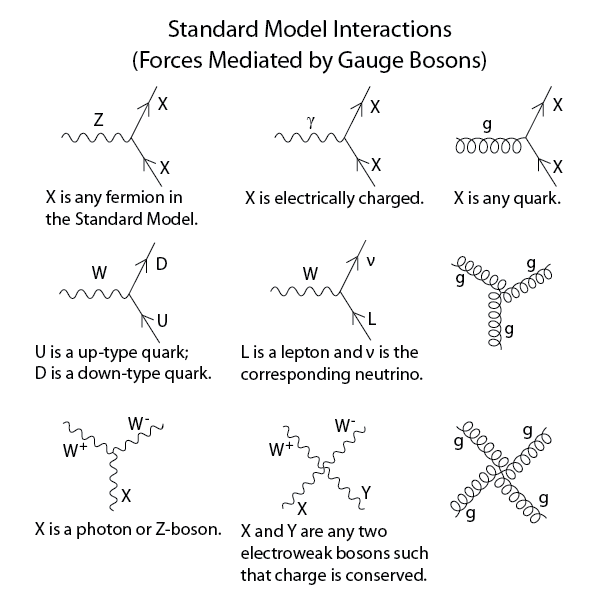
\includegraphics[width=0.6\textwidth]{/Users/rhombus/CMS/Thesis/thesis/pdfs/feyn/Standard_Model_Feynman_Diagram_Vertices.png}
    \label{fig:smcouplings}
\end{figure}
%%%%%%%%%%%%%
%%%%%%%%%%%%%
\begin{figure}[!htb]
 \center
 \caption[Feynman diagrams for $2\rightarrow2$ scattering]{
  Below are Feynman diagrams for $2\rightarrow2$ scattering. 
  These are the tree-level diagrams of the $s,t,u$
   channels respectively.
 } 
 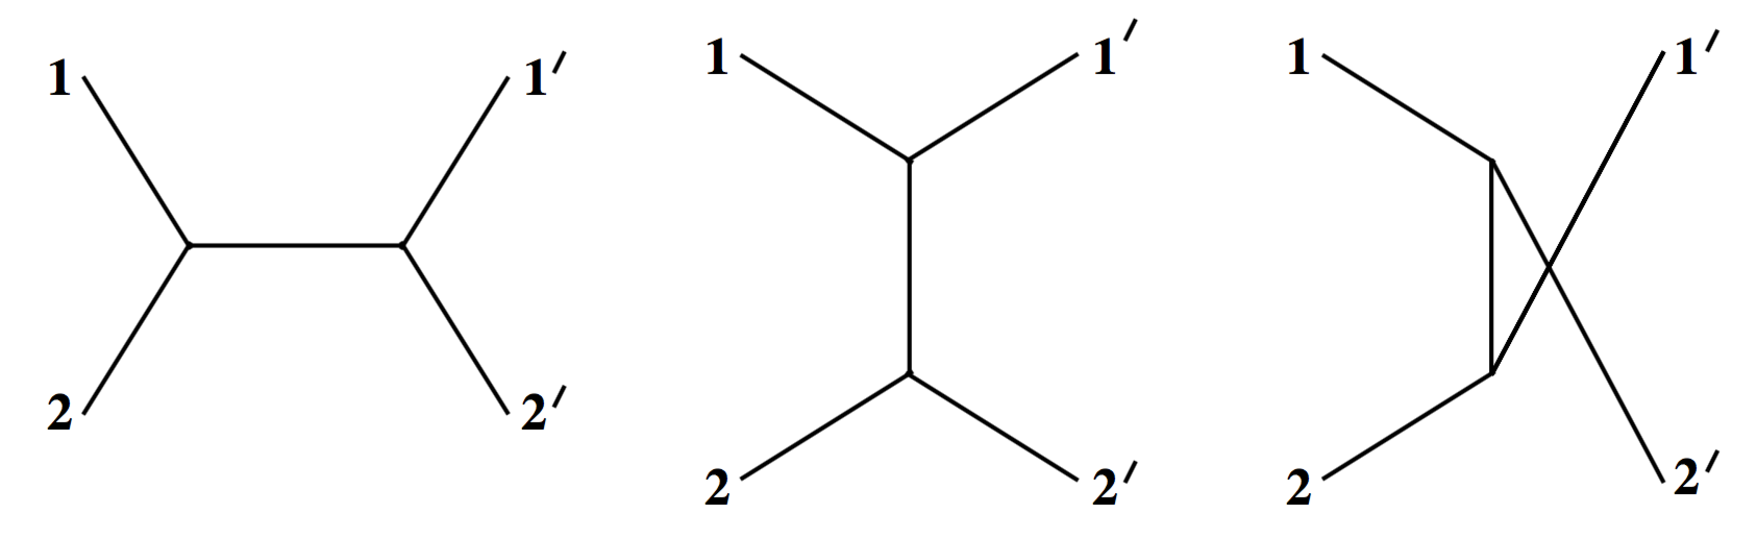
\includegraphics[width=0.6\textwidth]{/Users/rhombus/CMS/Thesis/thesis/pdfs/feyn/fenman2by2.pdf}
    \label{fig:fenyman2by2}
\end{figure}
%%%%%%%%%%%%%

\subsection{Renormalization}
 Crucial for the LSZ formulation are
  two features of quantum fields,
  that they are fully separable in the 
  infinite limit,
  $\langle 0 | \phi(x) | 0 \rangle = 0$,
  and that they are states of definite momentum,
  $ \langle k | \phi(x) | 0 \rangle = e^{-ikx}$.
 In the SM, which
  allows for fields to interact, these
  conditions are guaranteed by adjusting the
  strengths of the fundamental couplings, $g_1,g_2,g_3$.
 This ensures that the quantum states
  remain properly normalized, and is thus
  called renormalization.

 Renormalization is necessary to account
  for corrections to the tree-level propagators
  and vertices which arise from contributions
  of virtual particles connecting to 
  form closed internal loops.
 The lowest order, one-loop, diagrams
  are illustrated in Figure~\ref{fig:oneloopfeyn}.
 Renormalization is accomplished by introducing an energy scale,
  and assuming that the couplings are small compared 
  this this scale. 
 The coupling constants are therefore
  functions of energy 
  and are quoted at a particular renormalization scale,
  $\mu_R$.
 
 %% Determining if a theory is renormalizable
  % Srednicki 129, 18

 %% Consequences of running coupling constants ..

%%%%%%%%%%%%%
\begin{figure}[!tb]
 \center
 \caption[One-loop corrections to vertices and propagator]{
  Renormalization takes place via a modification
   of the coupling parameters $g_1,g_2,g_3$ to account
   for the contributions that loops of virtual
   particles make on the propagators and vertices.
  Below are diagrams keeping track of the
   flow of momentum for one-loop corrections to the 
   propagator and three and four point vertices.
 } 
 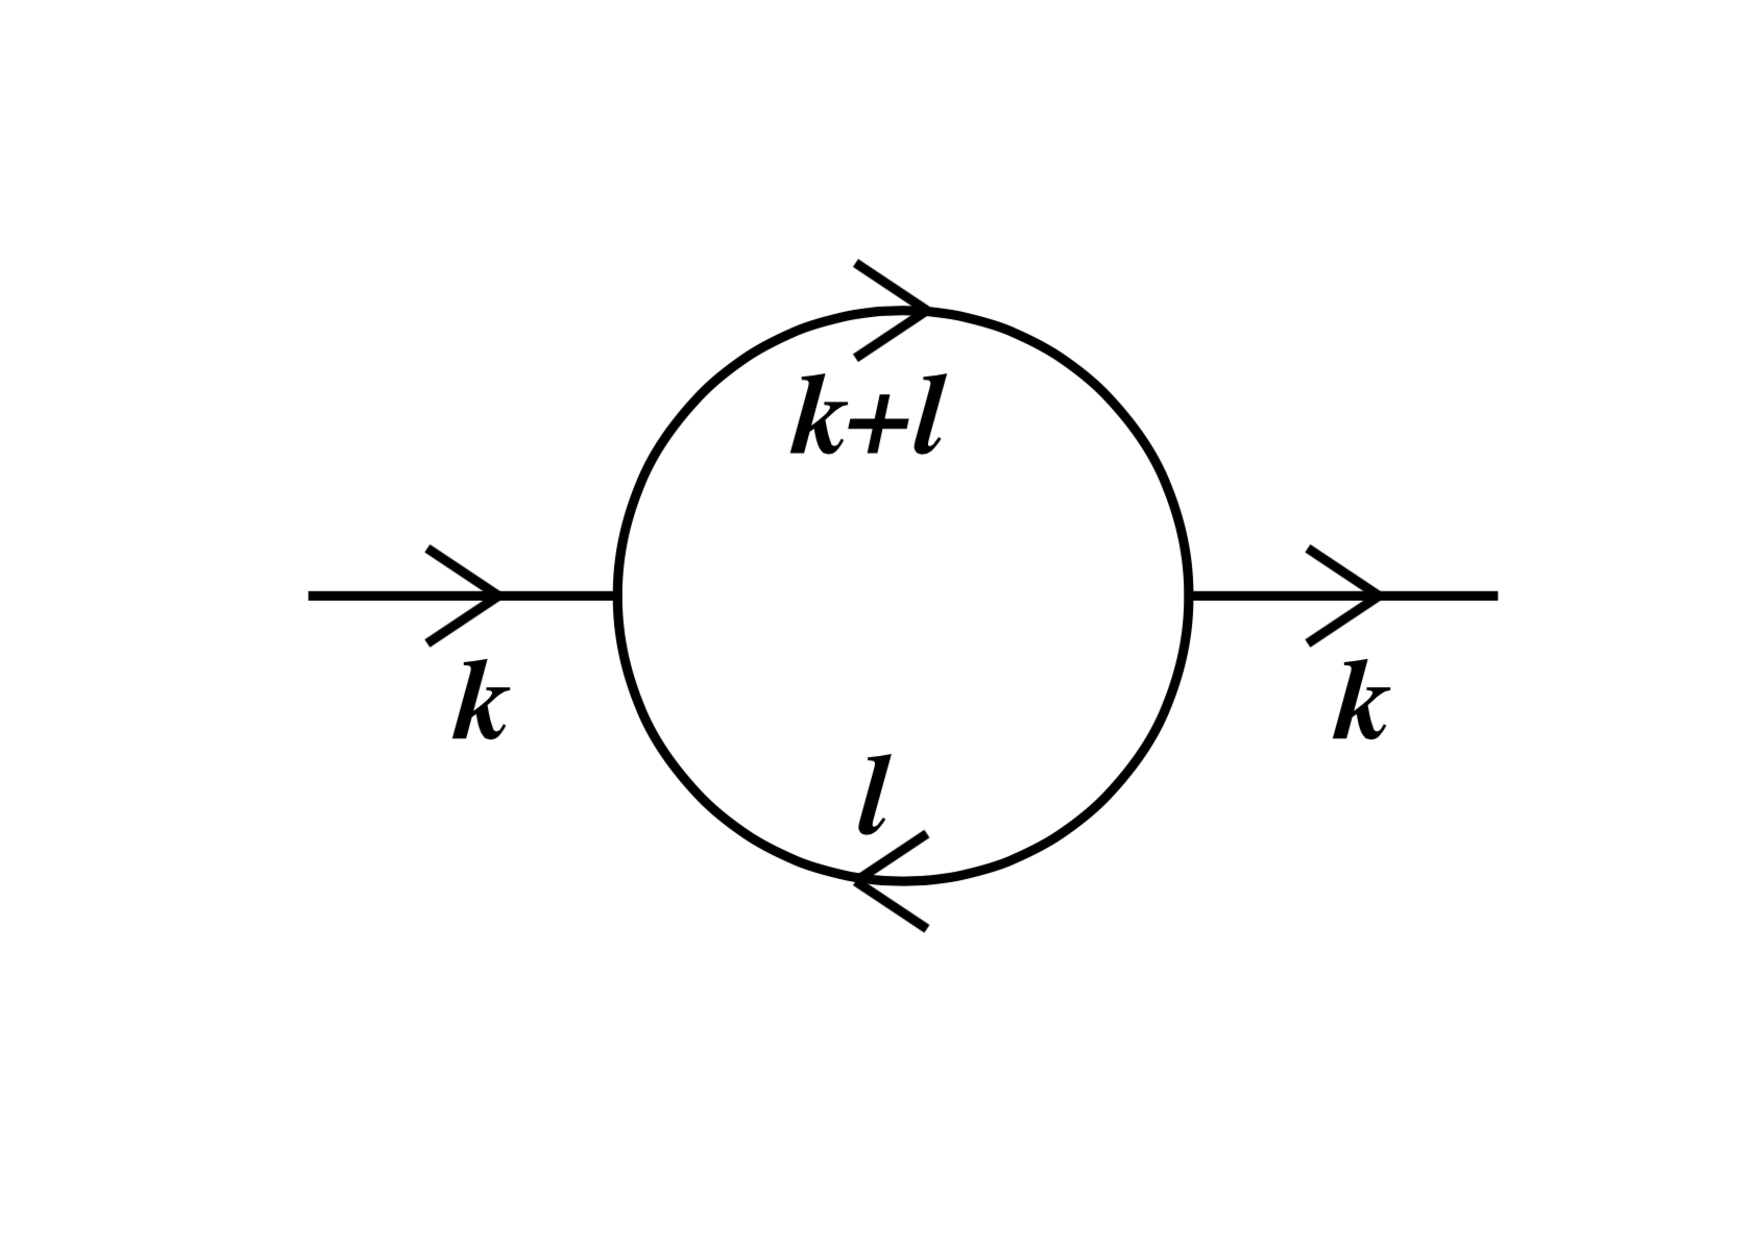
\includegraphics[width=0.3\textwidth]{/Users/rhombus/CMS/Thesis/thesis/pdfs/intro/loop_propagator.pdf}
 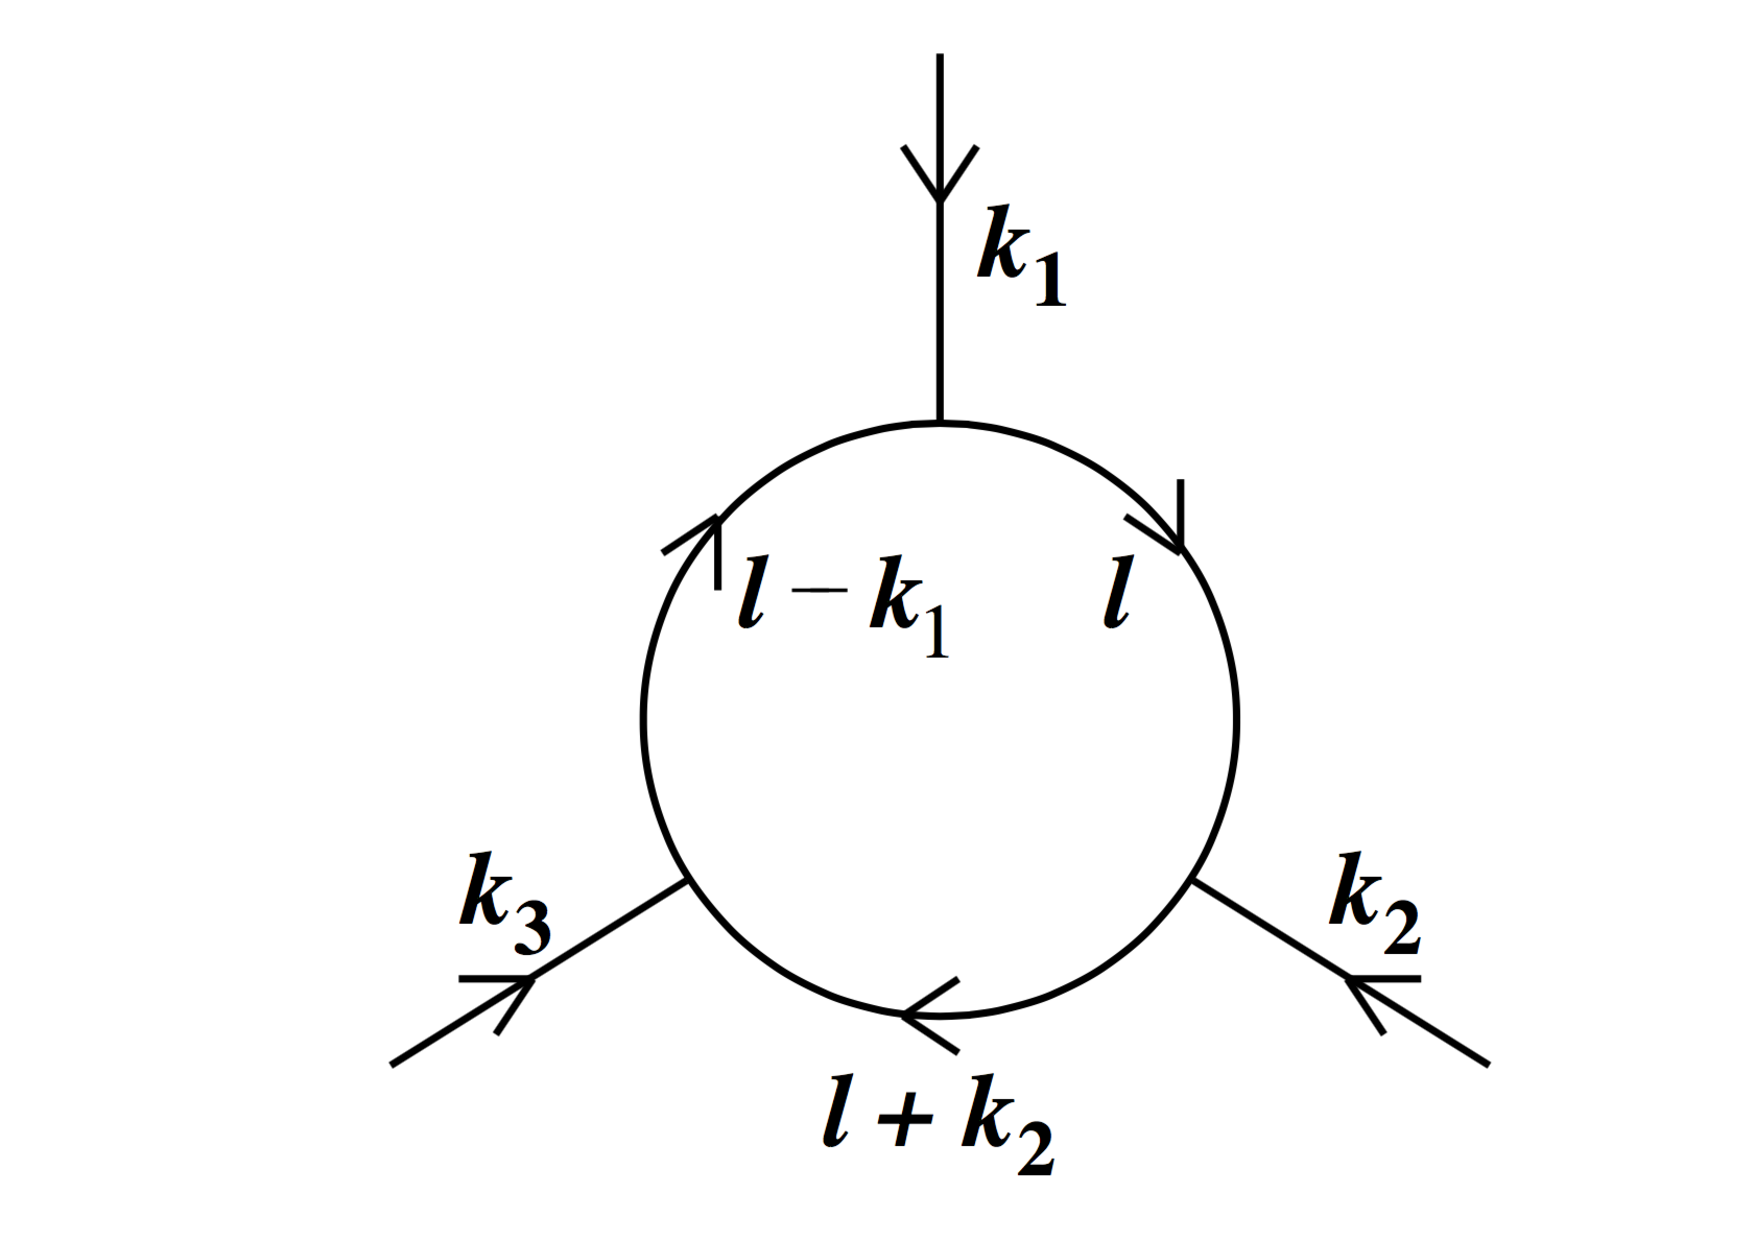
\includegraphics[width=0.3\textwidth]{/Users/rhombus/CMS/Thesis/thesis/pdfs/intro/loop_vertex.pdf}
 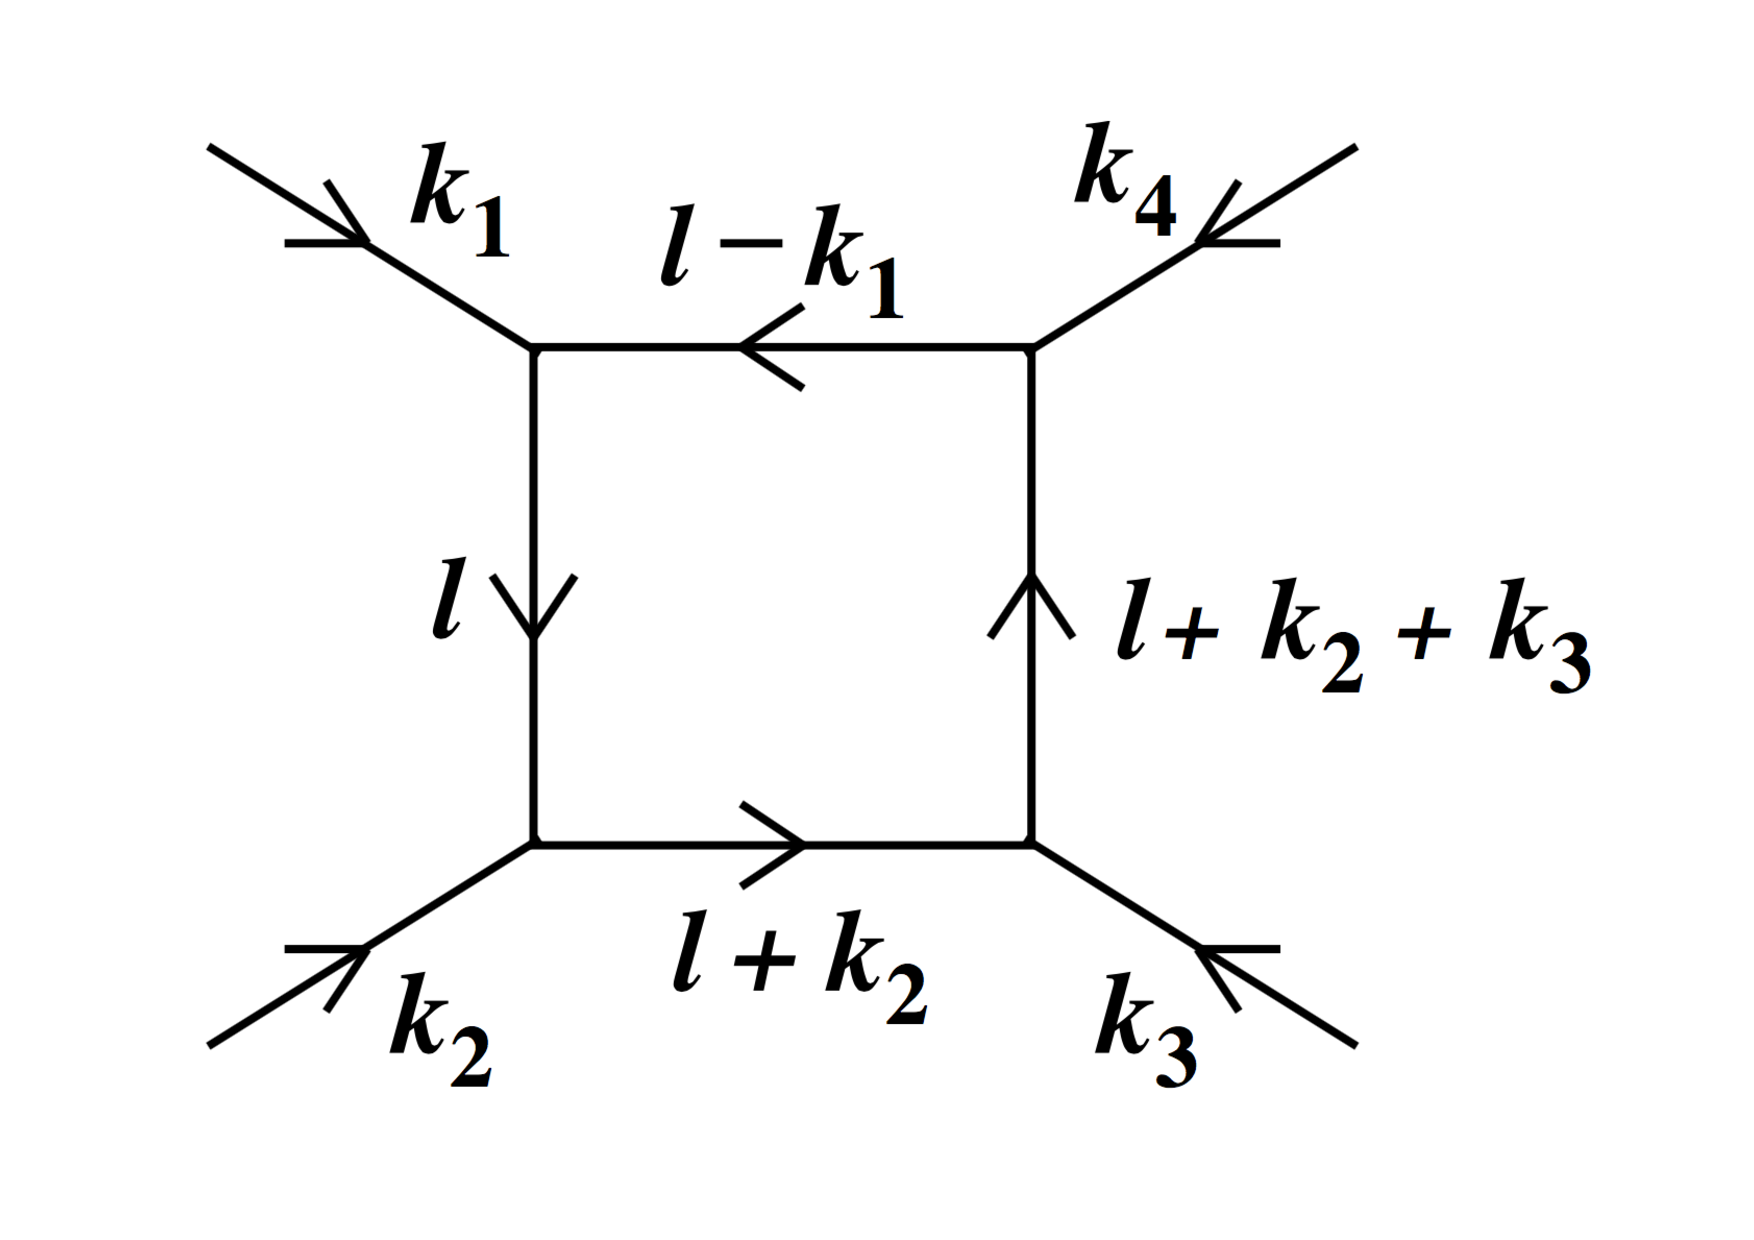
\includegraphics[width=0.3\textwidth]{/Users/rhombus/CMS/Thesis/thesis/pdfs/intro/loop_vertex4p.pdf}
    \label{fig:oneloopfeyn}
\end{figure}
%%%%%%%%%%%%%

%\subsection{Scattering amplitudes and cross sections}
\subsection{Cross sections and decay rates}

 The scattering amplitude $\langle f | i \rangle$
  is not a directly measurable observable.
 What can be observed is some finite distribution
  of data which may be analyzed to reveal
  information about the scattering amplitude.
 Quantum mechanics dictates that 
  only predictions of probability are possible,
  and the final probability of observing
  a particular interaction
  is dependent on many variables, including
  the energies, types and angular momenta of the incoming
  and outgoing particles as well as
  the masses of the propagators
  and the orientation and efficiency of the detector.

 A quantity typically measured is therefore the 
  interaction cross section, $\sigma$,
  and for the scattering of two incoming 
  particles going to $n'$ particles, $2\rightarrow n'$,
  in the CM frame, the differential is
\begin{equation}\label{eq:dsigma}
 d\sigma = \frac{1}{4\abs{\mathbf{k}_1}_{\mathrm{CM}}}\abs{\mathcal{T}}^2 
  d\mathrm{LIPS}_{n'}(k_1 + k_2)
\end{equation}
  where the scattering matrix element, $\mathcal{T}$,
  is defined using Equation \ref{eq:lszformula}, as 
\begin{equation}\label{eq:matrixelement}
\langle f | i \rangle = (2\pi)^4\delta^4\left(\sum k_{\mathrm{in}}-\sum k_{\mathrm{out}}\right)
  i \mathcal{T}
\end{equation}
  and the Lorentz-invariant measure of the 
  phase space for the $n'$ outgoing particles is
\begin{equation}\label{eq:dlips}
 d\mathrm{LIPS}_{n'}(k) = (2\pi)^4 \delta^4
  \left(k - \sum_{j=1}^{n'}k'_i \right )
  \prod_{j=1}^{n'}dq_j'
\end{equation}
 with the Lorentz-invariant differential $dq$.

 The cross section is used to calculate the rate
  at which a process occurs, but is
  not the only relevant factor in determining
  the overall production rate.
 The production rate of a given final state
  is also dependent on the incoming
  rate of possible interactions and is 
  known as luminosity, \lumi.
 Luminosity has the units of inverse area per unit time
  and the total number of events produced
  is therefore proportional to \tlumi.
 In any real detector, final state particles
  are collected only within a finite
  solid angle and the number of particles
  scattered into a given solid angle, $\Omega$, is given by
\begin{equation}\label{eq:lumidef}
 \frac{dN}{d\Omega} = \lumi \frac{d\sigma}{d\Omega}\;\;\;.
\end{equation}


 %The rate at which a particular event occurs
 % is proportional to \lumi and the cross section 
 % of that interaction, so it is the
 % (time) integrated luminosity that determines 
 % the total number of events produced.

 It is also possible for particles to decay
  as $1\rightarrow n'$.
 Massive particles decay to lighter ones
  in both the fermion and boson sectors,
  with all massive bosons able to 
  spontaneously decay via the diagrams in
  Figure~\ref{fig:smcouplings}.
 Of the charged fermions, only the first
  generation is stable for each type, and
  neutrinos are not known to spontaneously
  decay, but oscillate between flavors
  while propagating in free space.
 Like the differential cross section,
  the differential decay rate is a function
  of the scattering amplitude and
  has integration measure $d\mathrm{LIPS}$, 
\begin{equation}\label{eq:diffdecayrate}
 d\Gamma = \frac{1}{2E}\abs{\mathcal{T}}^2d\mathrm{LIPS}_{n'}(k)\;\;\;.
\end{equation}

 The differential decay rate is 
  inversely proportional to the energy
  of the particle, $E=\sqrt{m^2 + p^2}$.
 This means that
  comparatively heavy particles will decay
  faster than comparatively light ones
  and that energetic particles
  will appear to live longer 
  for a stationary observer due to
  relativistic time dilation effects.
 The total decay rate of a given particle
  is found by summing the decay rates from
  each of the contributing processes,
  and the primary decay channels and rates
  for the fundamental particles
  are given in Table \ref{tab:lifetimes}.

 At CMS, the heaviest quark and the heaviest
  lepton both decay before reaching
  the detector volume.
 This makes $b$ quarks the heaviest
  fundamental particles which can be seen
  to decay inside the detector,
  and therefore an object of interest.
 Additionally, their heavy mass means that they
  couple strongly with the Higgs boson
  which still has many properties that
  are under investigation.
 The $W$ and $Z$ bosons are both so 
  massive that they decay before reaching
  the innermost layers of the detector
  and are often identified by their decay products
  pointing back to a common vertex.
 
%%%% Table SU(2) Representations
\begin{table}[tb]
\caption[Fundamental particle decay channels and rates]
{
 Below are listed the decay channels and 
  rates for each of the unstable
  fundamental particles.
 At CMS, with the detection apparatus
  located a finite distance away from the
  interaction vertex, particles such as the
  $W$, $Z$ and Higgs bosons,
  as well as the $t$ and $tau$, decay before
  reaching the first layer of the detector.
}
\label{tab:lifetimes}
\begin{center}
\resizebox{\columnwidth}{!}{
\begin{tabular}{r|l|l|l}
Particle & Primary decay modes(s) & Total rest-frame $d\Gamma$ & Typical decay location \\
\hline\hline
$W$ & $W\rightarrow \ell\nu$ & X & Before reaching CMS \\
$Z$ & $Z\rightarrow f\overline{f}$ (for $2M_f < M_Z$) & X & Before reaching CMS \\
$\tau$ & $\tau\rightarrow W \nu_\tau$ & X & Before reaching CMS \\
$\mu$  & $\mu\rightarrow W \nu_\mu$ & X & After leaving CMS \\
$t$    & $t\rightarrow W^+b$ & X & Before reaching CMS \\
$b$    & $b\rightarrow W^-c$ & X & Inside CMS \\
$c$    & $c\rightarrow W^+s$ & X & Inside CMS \\
$s$    & $s\rightarrow W^-u$ & X & Inside CMS
\end{tabular}
}
\end{center}
\end{table}
%%%%%%%
 

\subsection{QCD and Proton Structure}\label{sec:protonstructure}
 The Feynman diagrams introduced in Section \ref{sec:PIandFD}
  describe the interactions between fundamental particles,
  but at the LHC, collisions take place between
  protons, which are composite.

 One feature of the $SU(3)$ symmetry of the
  strong force is that gluons
  carry one unit of color and one unit of anticolor
  while the quarks carry one unit of color charge.
 This is what allows gluons to interact with each other
  as well as with quarks.
 That quark confinement is necessitated by the $SU(3)$
  structure has not been conclusively determined, 
  but observationally, a free gluon or quark has 
  never been observed.
 Instead, quarks appear as bound in colorless (singlet)
  combinations called hadrons
  which are further classified as mesons ($q\overline{q}$)
  or as baryons ($qqq$ or
  $\overline{q}\overline{q}\overline{q}$),
  and are held together by gluons.
 Evidently, the binding energy of the
  quarks has a form such that
  after a distance of roughly $10^{-15}$ meters,
  the energy
  stored in the gluon field is greater
  than the energy needed to create a
  quark-antiquark pair, bringing the pair
  into existence.
 This process of energetic quarks
  creating particles as they
  separate is called hadronization
  and is an important effect at the LHC.

 Protons are a type of baryon and
  at low energy, may combine with a single electron 
  to form a neutral hydrogen atom.
 At higher energies, the internal structure 
  of the proton becomes more evident,
  and it contains three valence quarks, $uud$, 
  which are constantly exchanging gluons.
 When probed at high enough energy, or equivalently,
  at short enough length scales, these 
  gluons can also each split into a $q\overline{q}$ pair 
  which typically reannihialate with each other.
 With gluons inside the proton splitting into quarks
  and coupling with other gluons,
  this forms a `sea' of quarks and gluons,
  and as protons are accelerated
  to energies of \GeV or \TeV as is the case at the
  LHC, the fraction of the momentum of the
  proton attributed to the gluons becomes higher 
  than that attributed to the valence quarks.

 A proton-proton collider was therefore a 
  sensible choice for the LHC. 
 The physics goals of the project are
  to measure quantities associated with a wide range SM 
  processes and to continue the search for 
  evidence of new physics.
 Quarks interact with all of the SM gauge bosons
  as well as with the Higgs boson
  and the proton contains the lightest
  quarks of each type
  in addition to the gluons and sea.
 Colliding proton beams thus allow for
  the interactions between many different
  initial particle configurations to be explored,
  and with the exception of the neutrinos which 
  interact only via the weak exchange of the $Z$
  boson and escape the detectors,
  all other fundamental SM particles have been
  directly  observed  at CERN. 

\section{Dark Matter}
 \subsection{Experimental motivations}
  
 Albert Einstein's theory of general relativity, GR,
  has many experimental predictions which 
  run counter to human intuition.
 GR predicts that massive objects
  warp a four-dimensional spacetime and
  thus feel mutual attraction.
 This has as a consequence,
  the prediction that even massless objects
  such as photons will experience a 
  net deviation in their path
  near a massive object as a result of
  gravity and this effect was famously verified
  by Arthur Eddington
  through the observation of stars around the
  sun during a full solar eclipse. 
 More recently, the direct detection of
  gravitational waves by the LIGO
  Collaboration also aligns with the GR
  predictions of distorted spacetime
  around colliding black holes.
 The time distortion effects due to
  the varying strengths of Earth's gravitational
  field on the surface and at the GPS satellites,
  provide precise tests of the quantitative 
  predictions of GR.
 However, though these tests and others provide evidence that
  GR is an accurate theory of gravity,
  some basic predictions related to gravitational interactions 
  do not agree with observations,
  motivating the concept for DM.
  
 The first observational evidence for DM
  came from an analysis of the speeds of galaxies
  in the Coma cluster by Fritz Zwicky.
 The magnitude of the angular velocities of the
  galaxies was too great to be explained by the visible matter
  alone and DM is now believed to outweigh visible
  matter in a ratio of $5:1$ throughout the universe
  and $10:1$ throughout the Milky Way galaxy. 
  % http://map.gsfc.nasa.gov/universe/uni_matter.html

%[stability of spiral galaxies]
%
%[timescale of galactic formation / supergalactic structures]

  \subsection{Simplified theoretical models} 

  The defining features of DM are that
   it is massive and appears to interact
   on large scales only via the gravitational force.
  On the galactic and supergalactic scales,
   DM is distributed along similar structures
   as is visible matter, and it surrounds 
   visible matter in extended halos. 

  Because DM has not yet been observed, 
   the models of DM being considered in this thesis are
   simplified and based on minimal assumptions,
   the first being that DM is even capable of interacting
   with hadrons and is thus possible to produce
   at the LHC.
  While the visible sector of particles is diverse,
   the models used in this analysis
   consist of a single DM particle,
   $\chi$, which is assumed to be a fermion
   and may be different from $\overline{\chi}$.

  One way DM could couple to the SM is via the
   addition of a $U(1)$ symmetry that
   gives rise to a vector gauge mediator, $M$.
  If some quarks are also charged under
   $U(1)$, then DM may be produced in the
   $s$ channel as
   $f\overline{f}\rightarrow M\rightarrow\chi\overline{\chi}$.
  If $M$ conserves parity in $f\overline{f}\rightarrow M$,
   it is said to have a vector coupling,
   and if it violates parity, it is
   termed axial-vector.
  In these models, $M$ is assumed not
   to couple to leptons, but
   an effective field theory (EFT)
   model is also considered in this analysis
   which estimates a direct interaction
   between DM and photons. 
  This coupling is mediated by a vertex
   $\gamma\gamma\chi\overline{\chi}$.
   and allows for DM production via
   the channel
   $pp\rightarrow\gamma\rightarrow\gamma\chi\overline{\chi}$.





\chapter{Phenomenology of Processes}

\section[The Standard Model process \ppwbblnbb]
{The Standard Model process $\boldsymbol{\ppwbblnbb}$} \label{sec:wbbproduction}
%{The process $\boldsymbol{\mathbf{\ppwbblnbb}}$} \label{sec:wbbproduction}

The Feynman diagram depicting the full SM process \ppwbblnbb 
 along with the component vertices making it up
 are illustrated in Figure~\ref{fig:ppwbblnbbfeyn}.

%%%%%%%%%%%%%
\begin{figure}[!h]
 \center
 \caption[Feynman diagrams for \ppwbblnbb]{
  The Feynman diagram for the process
   \ppwbblnbb is illustrated below,
   and is composed from the individual vertices 
   illustrated on the left, each of which is
   described in Section \ref{sec:wbbproduction}.
 } 
\begin{tabular}{rl}
 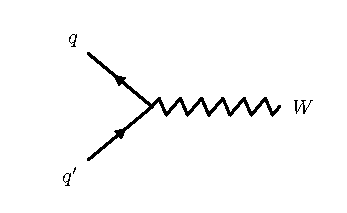
\includegraphics[width=0.3\textwidth]{/Users/rhombus/CMS/Thesis/thesis/pdfs/feyn/ppw/ppw.pdf} & 
 \multirow{3}{*}{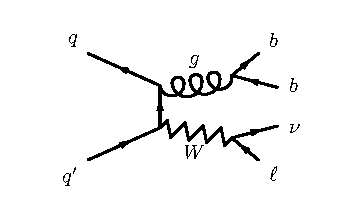
\includegraphics[width=0.6\textwidth]{/Users/rhombus/CMS/Thesis/thesis/pdfs/feyn/ppwbblnbb/ppwbblnbb.pdf}} \\
 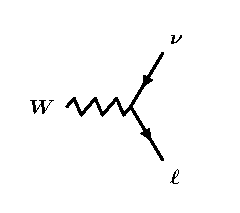
\includegraphics[width=0.3\textwidth]{/Users/rhombus/CMS/Thesis/thesis/pdfs/feyn/wln/wln.pdf} & {} \\
 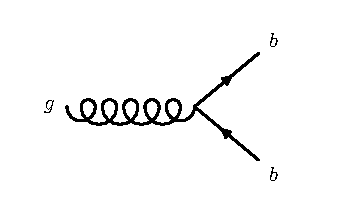
\includegraphics[width=0.3\textwidth]{/Users/rhombus/CMS/Thesis/thesis/pdfs/feyn/gbb/gbb.pdf} & {}
\end{tabular} 
    \label{fig:ppwbblnbbfeyn}
\end{figure}
%%%%%%%%%%%%%

 \subsection[\ppw]
 {$\boldsymbol{\ppw}$}

  The $W$ boson couples to all charged fermions
   and can be
   created during the collision of a quark-antiquark
   pair with a relative charge difference of $e$.
  In the proton are quarks and the most prevalent valence
   quark is the $u$.
  Therefore in a $pp$ collision,
   the channel by which most
   $W$ bosons are produced is
   via a the annihilation of a valence $u$ quark
   from one proton with 
   a $\overline{d}$ from the sea of the other,
   $u\overline{d}\rightarrow W^+$.
  Quarks of higher generation can also be found
   inside the sea as the result of gluons splitting into
   $q\overline{q}$ pairs, but all interactions
   are modified by a coefficient in the CKM matrix
   and higher generation mixing is thus suppressed.
  In this thesis, all modes of $pp\rightarrow W^\pm$ production are
   considered.

 \subsection[\wln]
 {$\boldsymbol{\wln}$}
  Just as the $W$ boson can be created by the
   collision $q\overline{q}'\rightarrow W$, 
   it can also decay as $W\rightarrow q\overline{q}'$.
  This is known as hadronic $W$ decay and
   can be a useful analysis channel for experimentalists,
   especially for decay products with energies approaching
   the \TeV scale.
  Leptonic $W$ decay, $\wln$, is also an important 
   channel for experimentalists and is the
   one considered in this analysis.
  Because leptons constitute a negligible fraction
   of the sea, the detection of leptons at high
   energy after a $pp$ collision is often a good 
   indicator of the decay of a massive gauge boson,
   $\wln$ or $Z\rightarrow \ell\overline{\ell}$.
  
  The $W$ boson is much heavier than any of the leptons
   and therefore decays with roughly equal probability
   to any of $e\nu_e, \mu\nu_\mu, \tau\nu_\tau$.
  From Table~\ref{tab:lifetimes}, tauons created
   at CMS
   subsequently decay before reaching the 
   detector, so for this analysis, the decay
   channel of the $W$ investigated is
   $\wln$ where $\ell\in e,\mu$.

 To reconstruct muons from the decay products,
  the transverse mass, $m_T$ variable is
  often used. 
 It is defined by
 $m_T^2 = m^2 + p_x^2 + p_y^2$
  where $p_i$ is the component of the momentum
  along the $i$ axis, and in the case of 
  a massive particle decaying to two massless
  particles, can be rewritten as
\begin{equation}
 m_T^2=2p_{T,1}p_{T,2}\left(1-\cos\phi\right)
\end{equation}
  where $\phi$ is the angle between the particles
  and $p_{T,j}$ is the component of the
  momentum of the particles in the transverse plane.

 In the decay of a $W$ boson, a neutrino 
  is produced, but can not be detected.
 The CMS detector is designed to
  capture the energy from all of the other 
  particles produced in a collision,
  so neutrinos are accounted for as \met.
 The variable \met is the
  transverse component of the negative
  vector sum of all of the 
  energy identified as having come from a particular
  interaction vertex,
  known as the primary vertex.
 Therefore the transverse mass of the $W$
  boson is 
\begin{equation}\label{eq:transversemass}
 \left(m_T^W\right)^2=2p_{T}^\ell\met\left(1-\cos\phi\right)
\end{equation}
  where $\phi$ is the angle between the lepton
  and \met.

 \subsection[\gbb]
 {$\boldsymbol{\gbb}$}
  Because quarks couple strongly to gluons
   and $q\overline{q}'\rightarrow W$ has been shown to be
   an important production channel in $pp$ collisions,
   it is possible for one of the
   initial state quarks to radiate a gluon.
  This is called initial state radiation, ISR,
   and if the gluon is produced with enough energy,
   it is capable of splitting to a quark-antiquark pair.
  In particular, a $g\rightarrow b\overline{b}$ vertex
   can be added to either of the incoming quarks to 
   form \ppwbblnbb.
  
  
%
% \subsection{b-jets}
%  quarks, jets/hadronization \\
%  heavy flavor - b quarks \\
%  displaced vertices
%

\section[The Standard Model process \ppzgnng]
        {The Standard Model process $\boldsymbol{\ppzgnng}$} \label{sec:znngproduction}

The Feynman diagram depicting the full SM process \ppzgnng 
 along with the component vertices making it up
 are illustrated in Figure~\ref{fig:ppzgnngfeyn}.

%%%%%%%%%%%%%
\begin{figure}[!h]
 \center
 \caption[Feynman diagrams for \ppzgnng]{
  The Feynman diagram for the process
   \ppzgnng is illustrated below,
   and is composed from the diagrams 
   illustrated on the left, each of which is
   described in Section \ref{sec:znngproduction}.
 } 
\begin{tabular}{rl}
 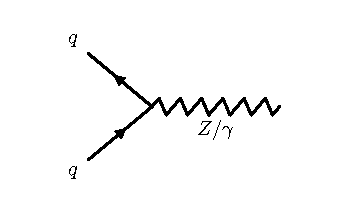
\includegraphics[width=0.3\textwidth]{/Users/rhombus/CMS/Thesis/thesis/pdfs/feyn/ppzsg/ppzsg.pdf} & 
 \multirow{3}{*}{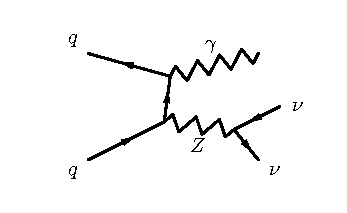
\includegraphics[width=0.6\textwidth]{/Users/rhombus/CMS/Thesis/thesis/pdfs/feyn/ppzgnng/ppzgnng.pdf}} \\
 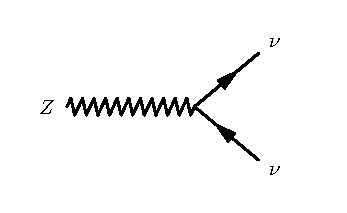
\includegraphics[width=0.3\textwidth]{/Users/rhombus/CMS/Thesis/thesis/pdfs/feyn/znn/znn.pdf} & {} \\
 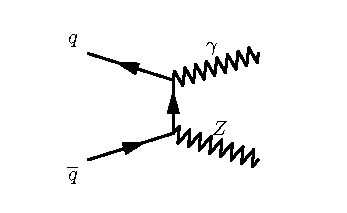
\includegraphics[width=0.3\textwidth]{/Users/rhombus/CMS/Thesis/thesis/pdfs/feyn/ppzg/ppzg.pdf} & {} 
\end{tabular} 
    \label{fig:ppzgnngfeyn}
\end{figure}
%%%%%%%%%%%%%

 \subsection[\ppzsg]
 {$\boldsymbol{\ppzsg}$}

 Similar to the $W$ boson, the $Z$ boson and the photon can
  also each be produced via the collision of quarks in
  the process $q\overline{q} \rightarrow Z/\gamma$.
 Unlike interactions with the $W$ boson, 
  interactions with $Z/\gamma$ conserve parity invariance
  and do not transport charge.
 Any interaction which can happen as mediated
  by a photon can also happen with the exchange
  of a $Z$ boson, but for collisions at $\sqrt{s}<M_Z = 90$ \GeV,
  the $Z$ can not be made on-shell.
 In this low energy regime $\gamma$ exchange dominates,
  but in 2015, the LHC ran at $\sqrt{s}=13$ \TeV
  and the relative mass difference between the $Z$ and the $\gamma$
  played a negligible role in their relative rates of production. 


 \subsection[\znn]
 {$\boldsymbol{\znn}$}

 The only particle which the $Z$ boson can couple to 
  but the photon can not is the neutrino.
 At $\sqrt{s}=13$ \TeV, the mass differences between
  the five lightest flavor of quark and the six 
  leptons are negligible and the $Z$ boson
  can decay into any kinematically allowed pairs,
  $Z\rightarrow f\overline{f}$.
 Including the three color possibilities
  for each quark, these are $3\times 5 + 6 = 21$ final states,
  each of which has roughly the same branching
  fraction. 
 Therefore only approximately $\sfrac{2}{7}$ of $Z$
  decays happen in the leptonic channel $Z\rightarrow \ell \overline{\ell}$.
  and of these decays, approximately $\sfrac{2}{3}$ happen
  as $Z\rightarrow \nu\overline{\nu}$.

 \subsection[\ppzgnng]
 {$\boldsymbol{\ppzgnng}$}

 With the photon coupling only to 
  electrically charged particles,
  the only place where a vertex
  containing a photon could be attached to
  either of the upper two left diagrams
  in Figure~\ref{fig:ppzgnngfeyn}
  is on one of the quarks.
 Photons are massless and therefore stable
  and so are a final state observable.
 Like the gluon in $\ppwbblnbb$,
  the photon is an example of ISR.
 In the CM frame of the colliding $q\overline{q}$,
  which is approximately the lab rest frame
  for colliding beams of equal energy as is the
  case at the LHC,
  conservation of momentum dictates
  that the $Z$ boson and photon should have 
  equal and opposite momenta.

 Unlike any of the other fermions, 
  neutrinos are electrically neutral
  and therefore only interact via
  the weak force. 
 So while the cross sections for
  most fermion-fermion interactions involve
  contributions from the comparatively stronger
  electromagnetic and strong forces,
  the neutrino cross section contains
  contributions from only the $W$ and $Z$
  bosons at tree-level and is
  much smaller than that of the charged fermions.
 This makes the detection of neutrinos very difficult in general,
  and impossible to do with present technology
  given the extreme backgrounds present
  in a collider setting.
%  and the Ice Cube dedicated neutrino detector encompasses
%  a cubic kilometer.
  
 In the case where the ISR photon is recoiling
  against a $Z$ boson which decays
  to neutrinos, 
  no direct detection of the $Z$ boson or of
  its decay products is possible,
  leaving only the photon visible in the final state.
 This is called the monophoton signature,
  where a photon is observed recoiling against
  apparently nothing, and while the
  monophoton signature is predicted to be
  observed as a result of SM process as in $\ppzgnng$,
  if the observed monophoton cross section is measured to be higher 
  than predicted, it could also be an indicator of physics beyond the SM (BSM).
 Specifically, the monophoton signature used in searches for dark matter.


 \section[Beyond the Standard Model: \ppgdm]
 {Beyond the Standard Model: $\boldsymbol{\ppgdm}$}

%%%%%%%%%%%%%
\begin{figure}[!h]
 \center
 \caption[Feynman diagrams for dark matter monophoton production]{
  Feynman diagrams for the DM process
   \ppgdm using simplified models
   are illustrated below.
  On the left is the $U(1)$ gauge
   model in which DM production
   is mediated by $M$ which can 
   be either vector or axial-vector,
   \ppgmgcc.
  On the right is the diagram for 
   DM production using an 
   EFT model of the $\gamma\gamma\chi\overline{\chi}$
   coupling, for the total process
   \ppggcc.
 } 
 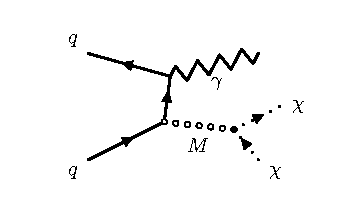
\includegraphics[width=0.4\textwidth]{/Users/rhombus/CMS/Thesis/thesis/pdfs/feyn/ppxg/ppxg.pdf}
 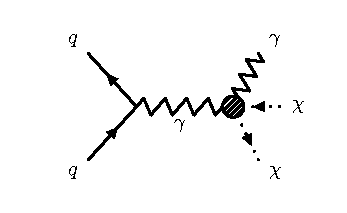
\includegraphics[width=0.4\textwidth]{/Users/rhombus/CMS/Thesis/thesis/pdfs/feyn/ppgx/ppgx.pdf}
    \label{fig:ppxgfeyn}
\end{figure}
%%%%%%%%%%%%%

 The existence of particle dark matter
  is well motivated, and the simplified
  model theories of DM used in this thesis allow
  for interactions which can result in
  the monophoton signature.
 One of the classes of models considered is a $U(1)$
  gauge theory in which $\chi\overline{\chi}$
  is produced via a vector or axial-vector mediator $M$
  which couples to quarks. 
 The tree-level process in this model which leaves
  a  monophoton signature 
  is illustrated on the left of
  Figure~\ref{fig:ppxgfeyn}, and the
  relevant parameters governing
  the cross section of this interaction are
  the masses of the two particles, $m_\chi$
  and $m_M$, and the strengths of the couplings
  between $M$ and quarks, $g_{Mq}$,
  and between $M$ and DM, $g_{M\chi}$.
 An EFT describing the four-point interaction
  vertex $\gamma\gamma\chi\overline{\chi}$ is also
  considered and illustrated on the right side of
  Figure~\ref{fig:ppxgfeyn}.
 In this theory, the coupling is a function
  of two parameters, $k_1$ and $k_2$,
  and is moderated by a mass scale, $\Lambda$.
 The other parameter in the EFT is $m_\chi$,
  and by measuring the cross section for
  \ppgdm in comparison with the SM prediction,
  estimations or limits can be set on 
  the parameters used in either of these
  two models.
  


\chapter{The LHC and CMS}\label{sec:experiment}
%\chapter{Experimental Setup}\label{sec:experiment}

The measurements presented in this thesis are performed
 on data of proton-proton collisions collected %in 2012 and 2015
 by the Compact Muon Solenoid (CMS) detector and
 provided by the
 Large Hadron Collider (LHC) at the 
 European Center for Nuclear Research (CERN).
The LHC was designed to probe physics at the 
 scale of \TeV and is capable of operating at
 multiple energy scales.
As measured in the CM frame
 of protons colliding inside CMS,
 the LHC operated at
 \s8 \TeV in 2012 and \s13 \TeV in 2015.
The measurement of the \ppwbb cross section 
 is performed using 19.8 \fbinv of integrated luminosity
 collected at \s8 \TeV and 
 the measurement of the \ppzgnng cross section
 and the extensions to set limits on DM models 
 uses 2.3 \fbinv of data collected at \s13 \TeV. 

\section{The Large Hadron Collider}
The LHC is a single-ring, double-bore 
 particle accelerator and collider located 
 on the border of France and Switzerland outside Geneva.
It was built using the existing 26.7 km of tunnels from the
 Large Electron Positron collider and hosts
 four primary experiments, located at four
 interaction points where beams of hadrons are made to cross.
Of the four experiments, two (CMS and ATLAS) are built for 
 studying SM processes and searching for new physics in general,
 one (ALICE) is designed to investigate 
 quark-gluon plasma resulting from 
 the high energy collisions of heavy ions such as lead,
 and one (LHCb) was built for the study of
 b-mesons and CP violation.

\subsection{LHC pre-acceleration}

To accelerate protons to their collision energy,
 a multi-stage procedure is used and 
 the major components of the accelerator infrastructure
 are illustrated in Figure \ref{fig:lhc_complex}.
First, protons are separated from
 electrons in neutral hydrogen gas before
 entering the linear accelerator (LINAC2)
 which brings them up to an energy of 50 \MeV
 using a series of oscillating electric potentials.
In this process, rather than having a continuous 
 stream of accelerating protons, the protons
 are grouped into bunches, and the beam
 retains this structure
 of distinct groups of protons separated by gaps
 throughout the acceleration procedure.
After the LINAC2, protons enter the Proton
 Synchrotron Booster (BOOSTER) where
 they are accelerated to 1.4 \GeV and 
 prepared for injection into the Proton Synchrotron (PS).
Inside the PS, bunches are accelerated to
 26 \GeV before being injected into the
 Super Proton Synchrotron (SPS) where they 
 are further accelerated to 450 \GeV.
After the SPS, bunches of protons are sent into
 the LHC.

\begin{figure}[htb]
\caption[The LCH accelerator complex at CERN]{
 Before protons are released into the LHC
  for final acceleration and collision, they pass through
  the LINAC2, BOOSTER, PS, and SPS, 
  undergoing acceleration %and collimation  
  at each stage.
 }
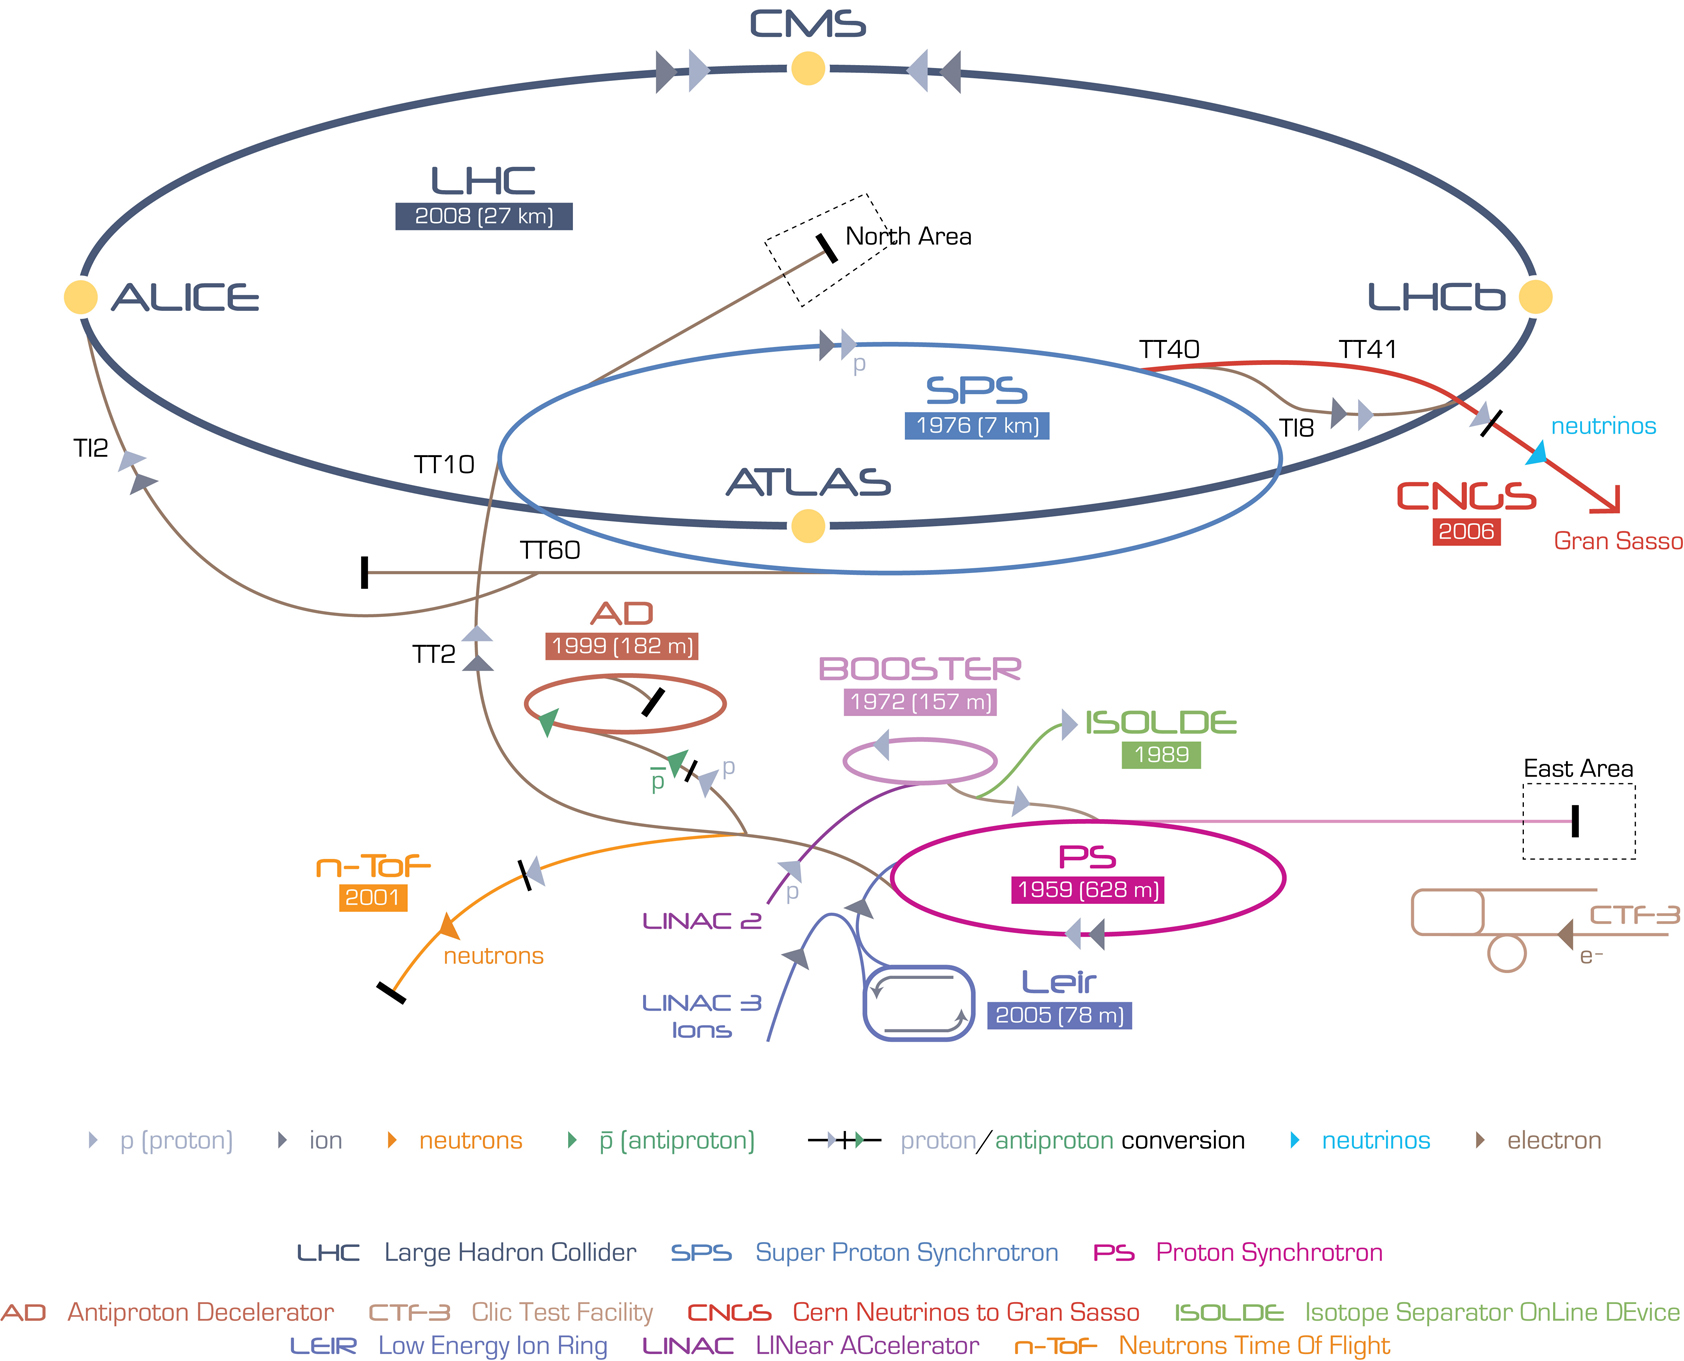
\includegraphics[width=\textwidth]{pdfs/experiment/cern_accelerator_complex.jpg}
\label{fig:lhc_complex}
\end{figure}


\subsection{LHC acceleration}
The work of accelerating and containing
 the protons which %circulate to 
 form %what is known as 
 the beam of
 the LHC is done by superconducting magnets. 
They are cooled to a temperature of 1.9 K
 using liquid helium and are housed in the
 LHC dipole apparatus diagrammed in Figure \ref{fig:lhc_dipole}.
The dipole contains two beam pipes which are
 each surrounded by superconducting coils
 of Niobium Titanium (NbTi)
 which carry oscillating currents when in operation.
These constitute RF cavities
 operating at 400 MHz and having the 
 ability to circulate proton
 bunches in opposing directions 
 between the two beam pipes
 with a spacing of 25 ns between bunches.
The magnets are capable of reaching 
 a strength of over 8 T, a constraint
 imposed by the desired energy scale 
 of the accelerator and the radius of the
 existing LEP tunnels
 in which the LHC was built.  
 
\begin{figure}[tb]
\caption[The LHC dipole]{
 Below is a cross section of the LHC dipole apparatus.
 It contains two beam pipes, each surrounded
  by superconducting magnetic coils
  which are held in place by an iron yolk.
 The system is cooled to a temperature of
  $1.9$ K and is thermally isolated 
  as well as protected from radiation.
 }
%\center
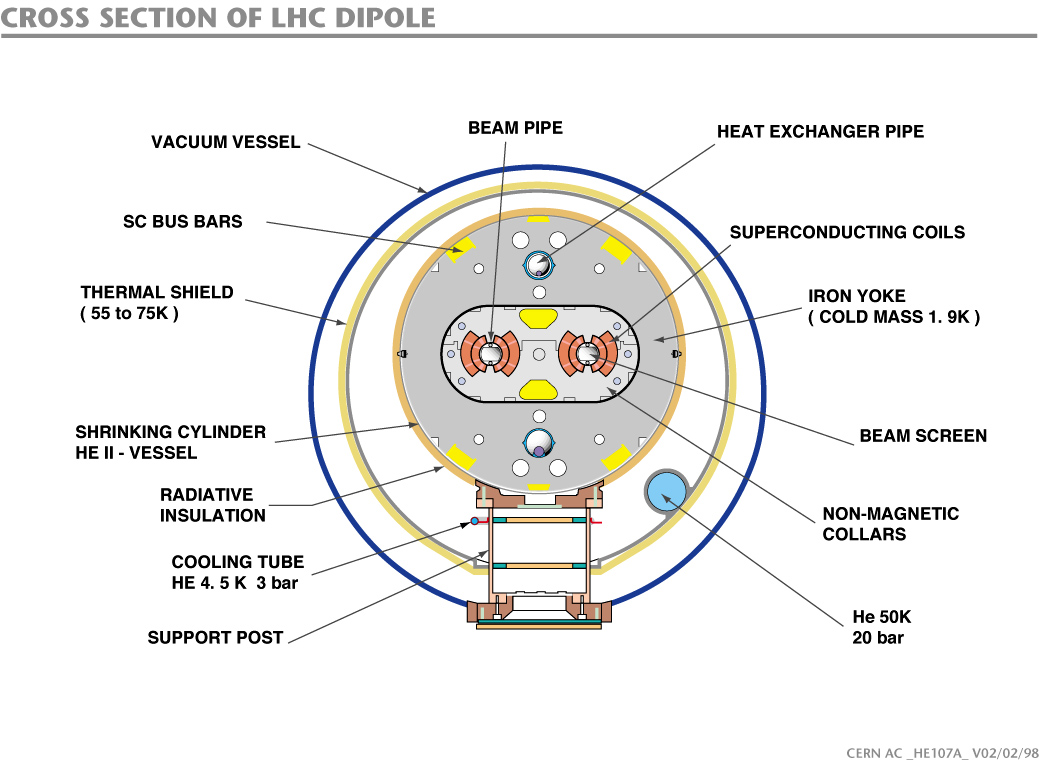
\includegraphics[width=\textwidth]{pdfs/experiment/lhc_dipole.jpg}
\label{fig:lhc_dipole}
\end{figure}

The Lorentz-invariant magnetic force on a
  particle of charge $q$, moving at
  velocity $\mathbf{v}$ in a 
  magnetic field $\mathbf{B}$ is
\begin{equation}\label{eq:bforce}
 \mathbf{F_B}=q\mathbf{v}\times\mathbf{B}
\end{equation}
 and the relativistic version of Newton's second
 law states
\begin{equation}
 \mathbf{F} = \frac{d\mathbf{p}}{dt} =
  \frac{d}{dt}\left ( \gamma m_0 \mathbf{v}  \right )
\end{equation}
 where $\gamma$ is the relativistic correction
 factor and $m_0$ is the rest mass of the particle.
These can be solved to find that the magnetic field
 required to hold a proton in planar
 circular motion as in the LHC is
\begin{equation}
 \mathbf{B}=\frac{p}{qR}
\end{equation}
 where $R = 4.3$ km.
At individual beam energies of 4 and 6.5 TeV
 in 2012 and 2015 respecyively,
 the rest mass of the proton constitutes
 a negligible fraction of the proton momentum
 and the minimum magnetic field required by the
 magnets is [todo - unit conversion].

The rate at which a particular collision 
 process occurs
 at the LHC is proportional to 
 the cross section of that interaction
 and the luminosity of the colliding beams
 as given in Equation~\ref{eq:lumidef}.
Assuming a Gaussian beam distribution,
 the machine parameters determine \lumi as

\begin{equation}\label{eq:lumi}
 \lumi=\frac{N_b^2 n_b f_{\mathrm{rev}} \gamma_r}{4\pi\epsilon_n \beta*}\mathcal{F}(\theta)
\end{equation}

 where $N_b$ is the number of particles per bunch,
 $n_b$ is the number of bunches per beam,
 $f_{\mathrm{rev}}$ is the revolution frequency of the bunches,
 $\gamma_r=E_p/m_p$ is the relativistic gamma factor
  for protons at energy $E_p$,
 $\epsilon_n$ is the normalized emittance which 
  characterizes bunch width,
 $\beta*$ is a measure fo the betatron oscillation envelope,
 and $\mathcal{F}(\theta)$ is a relativistic geometrical 
 correction factor which is a function of the
 angle at which the beams cross.
In addition to pushing the energy frontier,
 the LHC also has a significantly greater
 \lumi than previous hadron colliders. 
[Reference to Tevatron]
 
\section{The Compact Muon Solenoid Detector}

The CMS detector was built
 at Interaction Point 5 on the LHC ring
 to collect particle collision data  exploiting the full physics reach
 of the LHC.
The analysis of these data includes
 the discovery of the Higgs boson[REF]
 and high precision measurements of SM processes,
 as well as searches for physics beyond the standard model.
To be able to perform such precision measurements,
 CMS was designed with four main subdetectors 
 that work in concert and with a superconducting solenoid.
The tracking and most of the calorimetric
 detectors are inside the solenoid while
 the muon detectors are outside.
When running, the solenoid produces a 3.8 T 
 uniform magnetic field in its interior,
 and has a uniform 2 T field 
 over the bulk of the detector external to the solenoid.

The innermost of the subdetectors is the tracker
 which uses silicon pixel and strip detectors 
 to record the tracks of charged particles 
 passing through it. 
The tracks are used in conjunction with the
 $3.8$ T magnetic field to measure the momentum of these particles
 and
 this information is used for identifying
 the $pp$ interaction vertex %, defined as
 %the vertex having the highest pt sum of tracks
 as well as locating secondary vertices 
 from the decay of heavy flavor quarks
 such as the b or c.
Outside the tracker is the electromagnetic calorimeter (ECAL), 
 which is designed to have good energy resolution in recording
 the electromagnetic interactions of charged particles
 such as electrons or photons over a wide range of angles.
The hadronic calorimeter (HCAL) is outside the ECAL
 and is designed to absorb energy which
 comes in the form of neutral hadrons and provide 
 good resolution in missing transverse energy, \met.
Outside the calorimeters is the solenoid and steel return yolk,
 and the outermost layers of the detector are dedicated
 to the efficient detection of muons.
The overall length of CMS is 21.6 m, with a radius of 7.3 m
  and a total weight of 12500 tons.

\begin{figure}[tb]
\caption[The CMS Detector]{
 The CMS detector consists primarily of a tracker
  and electromagnetic and hadronic calorimeters
  which are mostly located inside a 3.8 T field provided
  by a superconducting solenoid,
  as well as a muon detection system located 
  outside the solenoid.
 }
%\center
\includegraphics[width=\textwidth]{pdfs/experiment/cms_explode.pdf}
\label{fig:cms_explode}
\end{figure}


 \subsection{Geometry} 
The coordinate system used by CMS is one in
 which the z-axis is aligned with the beam pipe,
 the y-axis is pointing upward vertically
 and the x-axis points radially inward toward the
 center of the LHC ring. 
The detector itself is mostly cylindrically symmetric
 about the beam pipe so cylindrical coordinates
 are also used.
In this system, $r$ is the radial distance
 as measured from the beam pipe, the azimuthal angle, $\phi$,
 is measured up from the x-axis in the x-y plane,
 and the polar angle, $\theta$, is measured
 down from the z-axis.
The angle $\theta$ is commonly replaced by pseudorapidity, 
\begin{equation}\label{eq:eta}
\eta = -\mathrm{ln}(\tan \theta/2)
\end{equation}
 since the distribution of particles
 is roughly constant as a function of $\eta$.
For the calorimeters, "barrel" refers to the region of $|\eta| < 1.4442$,
 and "endcap" to the region $3.0 > |\eta| > 1.566$.
Instrumentation cables are run through the
 gap between the barrel and endcap,
 so this area has detecting components. 
The HCAL forward region covers $3.0 < |\eta| < 5$ and
 the tracker extends to $|\eta| < 2.5$.

 \subsection{Magnet}
To precisely measure the momentum of a charged particle, 
 it is necessary to measure radius of curvature 
 of that particle as it moves through a magnetic field.
The momentum resolution varies as 

\begin{equation}\label{eq:res_mag}
\frac{\delta p}{p} \sim \frac{1}{L^2B}
\end{equation}
 where $L$ is the length of the track of the 
 particle through a magnetic field of
 strength $B$.
For particles at high energy, this requires a very strong
 magnetic field which is achieved by the superconducting 
 solenoid in CMS.
The solenoid operates at 3.8 T with 
 a bore of 3 m in radius and 12.5 m in length
 and is constructed from four layers of NbTi superconductor.
The steel yoke which provides physical support for the 
 CMS structure and serves as an absorber for the
 muon system is fully saturated by the fringe magnetic field
 from the solenoid.

 \subsection{Tracking System}
The inner tracking system of CMS is designed to provide
 precise and efficient measurements of the trajectories
 of charged particles produced during collisions,
 as well as a precise reconstruction of secondary vertices.
The tracker has a length of 5.8 m and a radius of
 1.25 m in a cylindrical structure surrounding the 
 interaction point, as illustrated in Figure \ref{fig:tracker}.

At the core of the tracker and closest to the beam line
 are three concentric cylindrical layers %4.4, 7.3, 10.2 cm 
 of hybrid pixel detector modules which are complemented
 by two discs of pixel modules on each end
 and extend a to a distance of 10 cm from the beam line.
[TODO - Explain - silicon]
In total, the pixel component of the tracker covers
 an area of about 1 m$^2$ with 66 million pixels.
External to the pixel detector are the tracker inner barrel and discs (TIB/TID)
 which are made from silicon strips and extend 
 out to a distance of 55 cm.
There are four layers of strips in the TIB, with 3 discs at each end.
The tracker outer barrel (TOB) is composed of
 6 layers of micro-strip sensors and extends
 in z between $\pm$118 cm and to a radius of 116 cm.
At the end of the z range for the TOB are the
 tracker end caps (TEC) which cover the ranges
 $124<|z|<282$ cm and 22.5 cm $<r<$113.5 cm.
Each TEC is composed of 9 discs,
 each carrying up to 7 rings of silicon micro-strip detectors.
In total, the tracker contains 9.3 million strips
 which cover an area of 198 m$^2$ and extends
 to an acceptance of $|\eta|<2.5$.
For tracks with momentum on the order of 100 \GeV,
 the momentum resolution is around 1-2\% up to $|\eta|<1.6$
 and degrades to around 10\% with increasing $\eta$.

\begin{figure}[tb]
\caption[The CMS Tracking System]{
 Below is a schematic of the CMS tracking system
  where each line represents a detector module.
 The system is made from silicon pixels and
  silicon microstrips distributed into four sections,
  TIB, TID, TOB, TEC.
 }
%\center
\includegraphics[width=\textwidth]{pdfs/experiment/cms_tracker.pdf}
\label{fig:tracker}
\end{figure}
 

 \subsection{Electronic Calorimeter}

The electronic calorimeter (ECAL) is a homogeneous
 calorimeter made from nearly 76000 crystals of lead tungstate (\pbw)
 mounted in the barrel and endcap sections with a 
 preshower detector located in front of the endcaps,
 arranged as shown in Figure \ref{fig:ecal}
In the barrel, avalanche photodiodes are used as photodetectors, 
 and in the endcap vacuum phototriodes are used. 
The material \pbw was chosen for its properties of being
 dense, optically transparent and radiation hard. 
The radiation length inside the ECAL is typically less than 1 cm
 with a Moliere radius of 2.2 cm and about 80\% of the
 light is emitted from a crystal within the first 25 ns.
Since the length of a given crystal is on the order of 20 cm,
 most photons and electrons deposit all of their energy 
 within the ECAL, and do not reach the HCAL.

The use of \pbw crystals allows for excellent position and timing resolution
 with the energy resolution given by 

\begin{equation}\label{eq:ecal_res}
 \left(\frac{\delta_E}{E}\right) =  \left(\frac{2.8\%}{\sqrt{E}}\right)^2 + \left(\frac{0.12}{E}\right) + (0.30\%)^2 .
\end{equation}
 
In this expression, the first term comes from the statistical error 
 in the measurement which arises
 from the stochastic nature of electromagnetic shower evolution
 and the second term represents the error in the measurement
 which results from noise in the electronics or
 energy deposits from additional soft interactions.
The ECAL provides stable and accurate
 measurements of energies over a range from 1 \GeV to 1 \TeV, 
 with the upper limit set by the energy at which electromagnetic showers
 penetrate through the ECAL into the HCAL.
[REF][TODO - how much?]
With time, after undergoing a heavy bombardment of high energy radiation,
 the \pbw crystals physically deteriorate and develop 
 nonuniform light transmission properties.
[REF] 
This is monitored and corrected for using a laser calibration system
 that probes for changes in crystal transparency.
 %during the running of the LHC.

\begin{figure}[tb]
\caption[The CMS Electromagnetic Calorimeter]{
 Below is a diagram of the ECAL, 
  which sits between the tracker and HCAL in CMS.
 It is made from \pbw crystals throughout the volume
  with avalanche photodiodes in the barrel
  and vacuum phototriodes in the endcaps.
 }
%\center
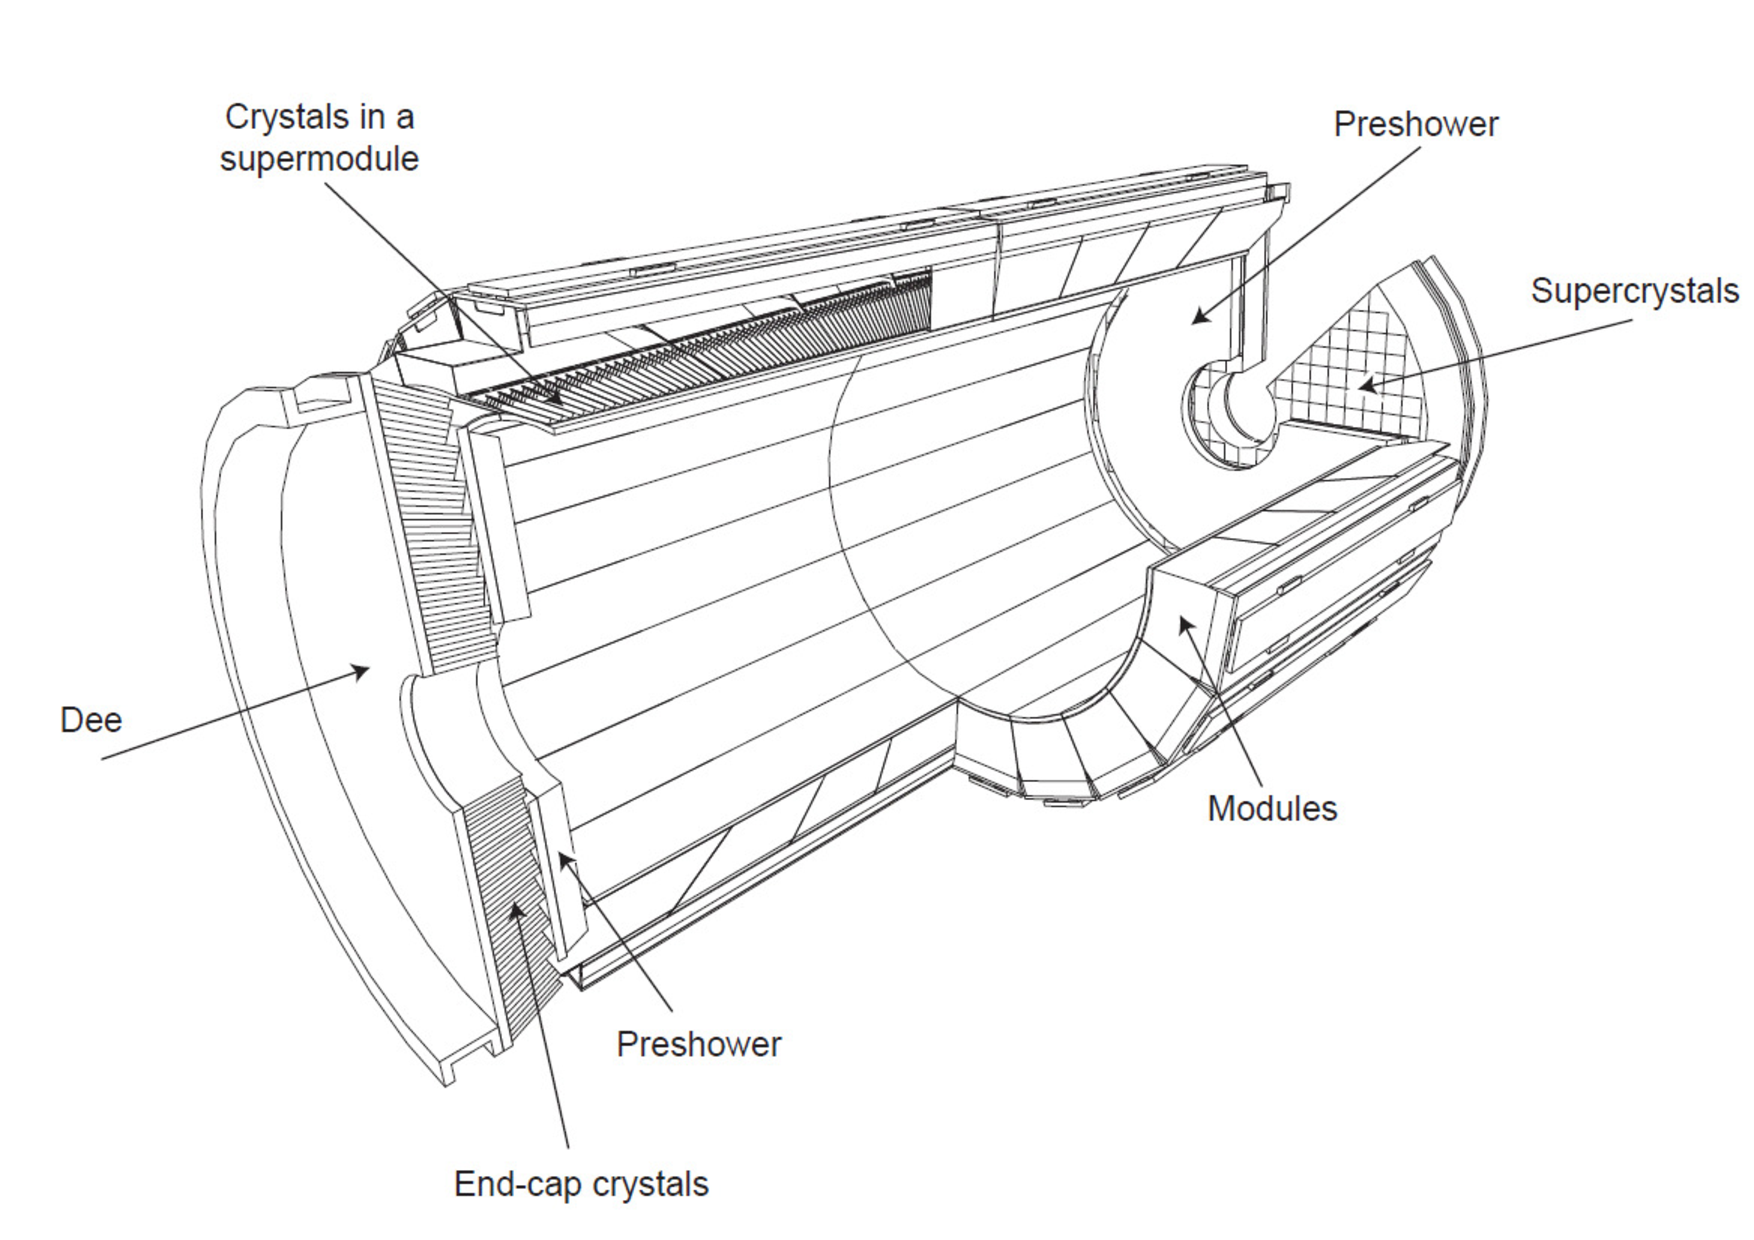
\includegraphics[width=\textwidth]{pdfs/experiment/cms_ecal.pdf}
\label{fig:ecal}
\end{figure}
 

 \subsection{Hadronic Calorimeter}
Situated mostly between the ECAL and the superconducting solenoid
 is the hadronic calorimeter (HCAL) which plays a
 crucial role in the measurement of hadron jets
 and particles such as neutrinos which escape the detector
 and result in apparent missing transverse energy.
The HCAL is designed to contain the energy of neutral
 particles which pass through the ECAL and is therefore made
 from dense materials such as 
 steel and brass interleaved with scintillating material.
Because the HCAL is designed to fit between these
 two components, it takes the shape of a hollow
 cylinder of inner radius 1.77 m and outer radius 2.95 m
 and one half of the HCAL is illustrated in Figure \ref{fig:hcal}.

The barrel of the HCAL (HB) extends to $|\eta|<1.3$ 
 and is constructed from brass absorber plate wedges aligned parallel 
 to the beam axis and mounted in an overlapping configuration,
 with a smaller amount of steel used in the inner and outermost
 wedges for structural stability.
The endcap of the HCAL (HE) extends this coverage to $|\eta|<3.0$
 and is complemented by the forward hadron calorimeter (HF)
 which is made from the comparatively radiation-hard 
 steel plates embedded with quartz fibers.
Inside the barrel region there is an additional layer of the
 HCAL, the outer calorimeter (HO), which is located just
 outside the solenoid and uses it as an absorber 
 for energetic showers which start late in the HB.

In the HB, HO and HE, light from particle showers
 [TODO - not exactly ..] 
 inside scintillators and collected by quartz fibers
 and then used as an estimate of the total energy of the shower.
In the HF, this estimate is made using the Cherenkov 
 radiation from particles with energy above 190 \keV
 collected by the quartz fibers.
For the two cases, the energy resolution takes the same
 functional form 

\begin{equation}\label{eq:hcal_res}
 \left(\frac{\delta_E}{E}\right) =  \left(\frac{A}{\sqrt{E}}\right)^2 + (B)^2 
\end{equation}
 where $A$ is 90$\%$ (172$\%$) in the HB/HO/HE (HF)
  and relates to the stochastic uncertainty of shower evolution
 and $B$ is 4.5$\%$ (9.0$\%$) and comes from uncertainties in calibration.


\begin{figure}[tb]
\caption[The CMS Hadronic Calorimeter]{
 A schematic layout of the HCAL, which complements the ECAL
  in providing a measurement of the total energy produced 
  in a collision.
 The HCAL is made from brass and steel plates,
  embedded with quartz fibers.
 }
%\center
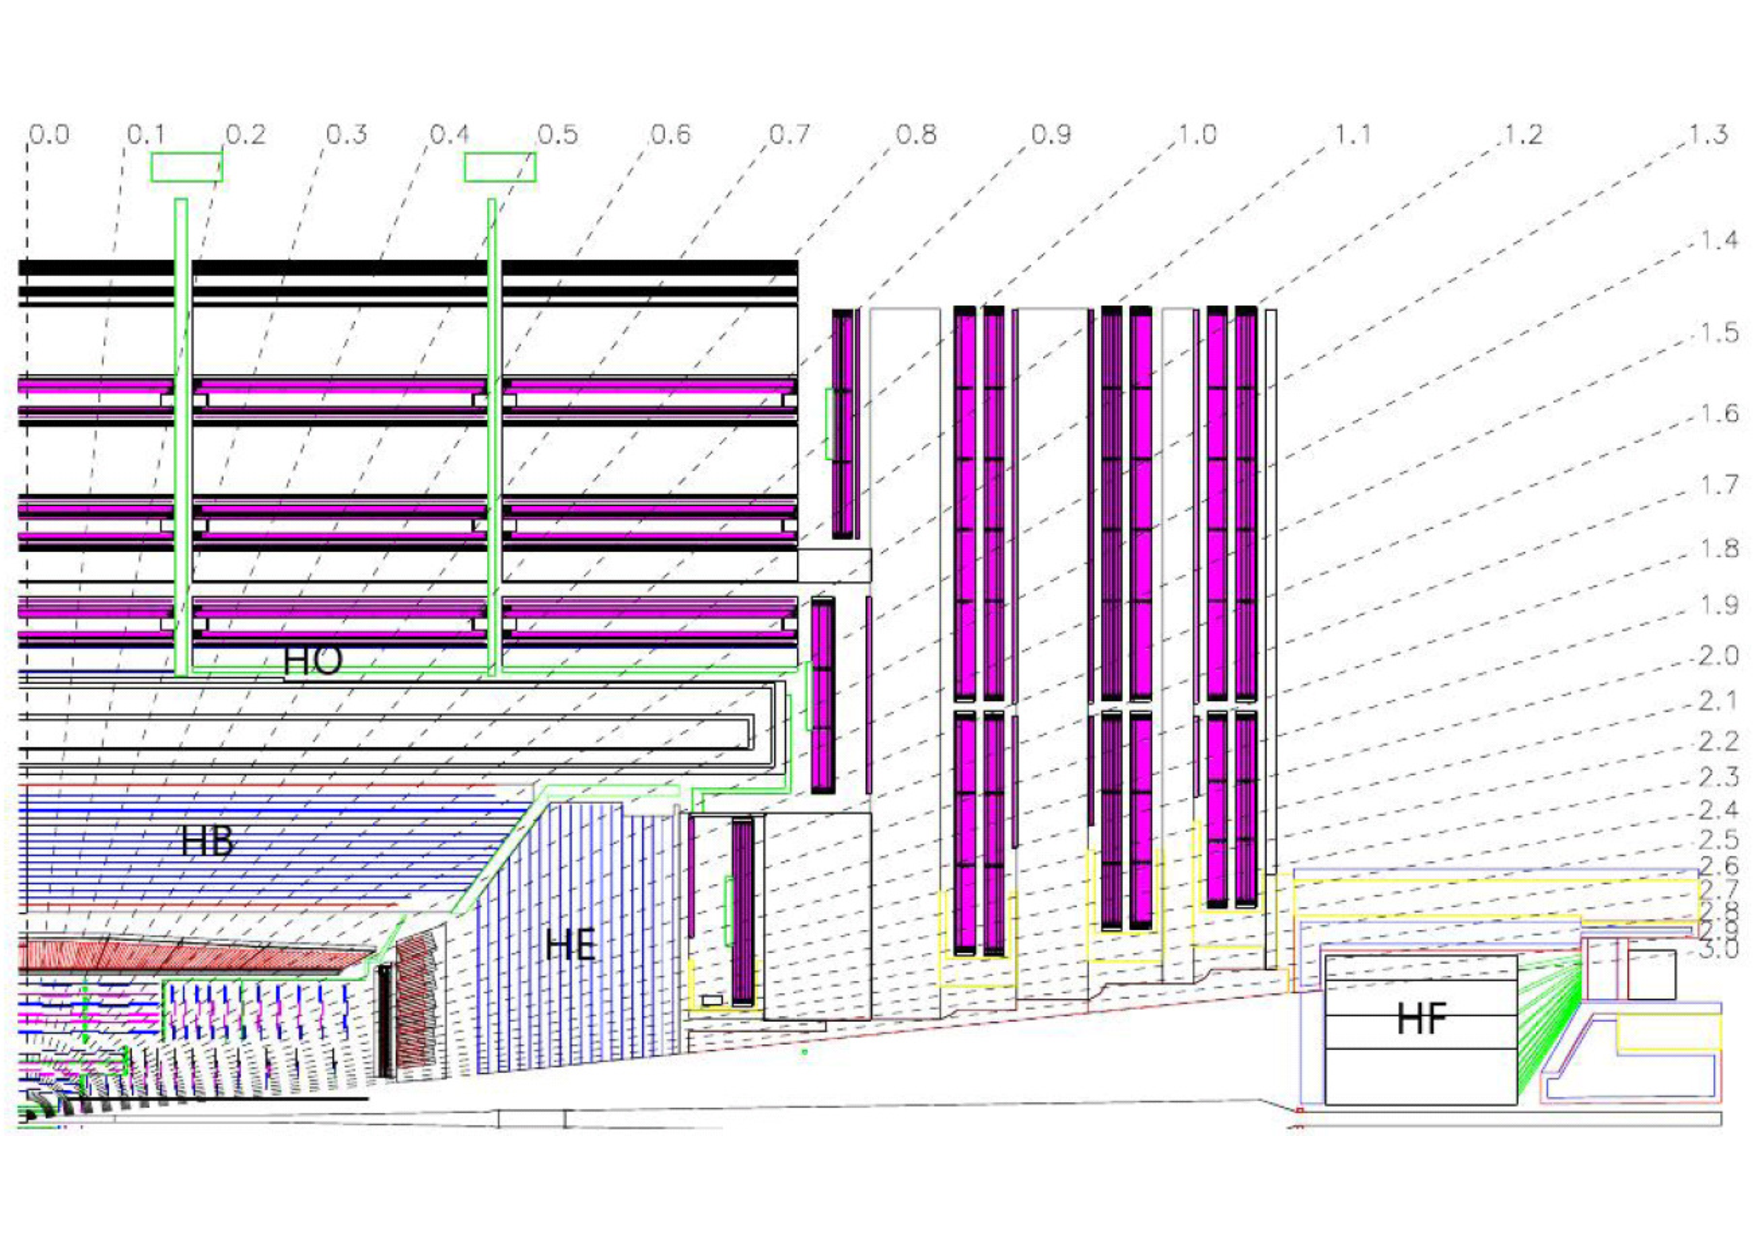
\includegraphics[width=\textwidth]{pdfs/experiment/cms_hcal.pdf}
\label{fig:hcal}
\end{figure}
 

 \subsection{Muon System}

Muons play a central role in the physics program outlined
 by CMS and the muon detection system is positioned 
 as the outermost layer of the detector. 
Unlike the other charged leptons, 
 muons typically pass through the ECAL and HCAL and
 deposit only a fraction of their energy, so
 a dedicated muon system is necessary in order to
 determine the momentum of these particles.
The muon system is composed of three different kinds
 of gaseous detectors,
 drift tubes (DTs), resistive plate chambers (RPCs)
 and cathode strip chambers (CSCs) and their layout is
 illustrated in Figure \ref{fig:muon}.

The barrel region of the muon system is covered by DTs
 in the range $|\eta|<1.2$ and the endcaps are covered 
 by CSCs in the range $0.9<|\eta|<2.4$.
The RPCs are located
 in the range $|\eta|<1.6$ and provide fast,
 independent and highly segmented transverse
 momentum measurements of muons. 

The DT system is composed of 4 stations which 
 form concentric cylinders about the beam line
 and contain 172000 sensitive wires. 
As charged particles enter the DTs,
 they ionize the Ar/CO$_2$ gas mixture,
 knocking off electrons  which 
 then are attracted to the positively charged wires.

The CSCs are less sensitive to uneven magnetic fields
 and high particle rates so are therefore used in the endcaps.
They are made from crossed arrays of positively 
 charged wires and negatively charged strips
 in gas and are composed
 of six layers, giving them precise timing
 as well as positional information. 
As an upgrade between the 2012 and 2015 data taking periods,
 a fourth layer of CSCs was added to the CMS detector, 
 adding to the three which were present in 2012.

The RPCs are built from two sheets held at opposite
 charges and separated by a gas volume.
As muons move through the chamber, electrons
 are ionized from the gas and attracted to small
 metallic strips which they reach after a small
 but well known time delay. 
The timing resolution of RPCs is on the order of 1 ns. 

\begin{figure}[tb]
\caption[The CMS Muon System]{
 The CMS muon system uses DTs, RPCs,
  and CSCs to provide muon detection
  up to $\eta < 2.4$.
 Shown below is the geometrical arrangement
  of the different muon
  subsystems and how they fit with
  the rest of the CMS detector.
 }
\label{fig:muon}
%\center
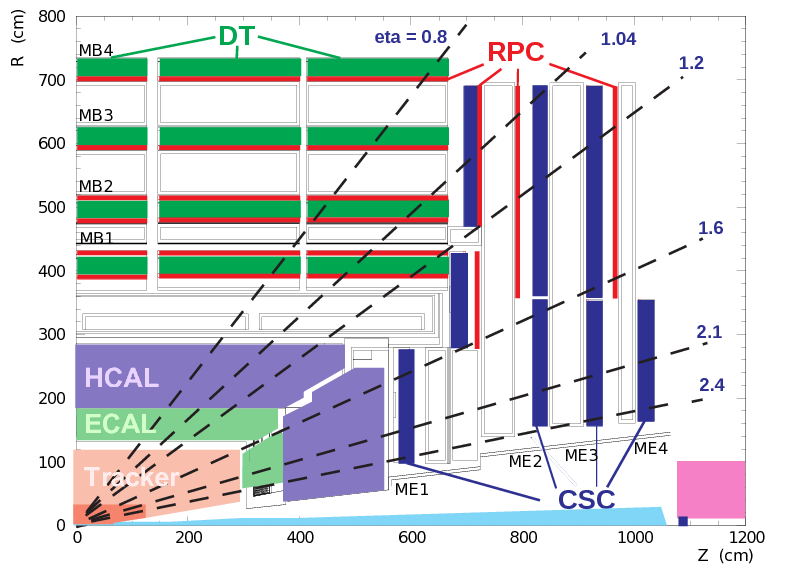
\includegraphics[width=\textwidth]{pdfs/experiment/cms_muon.png}
\end{figure}
 
\subsection{Trigger and Data Acquisition}



  


\chapter{Event Simulation and Reconstruction}\label{sec:simulation}
%%%%%%%%%%%%%
\section{Simulation of Events}
 Vital to the analysis of the data
  gathered using the CMS detector
  are accompanying predictions to be compared against.
 Good predictions can be used not only 
  for direct comparison against data
  as in the case of a cross section measurement,
  but can also be used in the design of 
  future detectors and experiments,
  or for optimizations of parameters in blinded analyses.
 Predictions are made by 
  simulating $pp$ collisions and the subsequent
  decays and interactions that take place
  inside the CMS detector volume
  using Monte Carlo (MC) techniques.
 The first step in producing these simulations
  is the generation of the collision event
  itself, and the second
  is in simulating the interaction of the
  collision products with the detector.

\subsection{Monte Carlo Event Generation}
 There are two complimentary methods used
  in producing a simulation of the 
  collision event, the direct calculation 
  of a scattering amplitude
  (also known as a matrix element, ME),
  and the showering of particles as they
  decay, hadronize and radiate.

 As discussed in Section~\ref{sec:protonstructure},
  protons are composite objects which form
  as the result of strong 
  interactions between bound quarks.
 Protons are therefore modeled using 
  parton distribution functions (PDFs)
  which describe the probability of
  finding a given constituent particle,
  or parton, to contain a given fraction
  of the momentum of the proton.
 The PDF is thus actually a set of density functions,
  one for each parton taken into account,
  and examples of the CTEQ6M parton distribution
  function at two values of of momentum transfer, $Q$,
  are shown in Figure~\ref{fig:cteqpdfs}.
 Weighted with probabilities from the PDF set
  and summed over,
  MEs are calculated explicitly from Feynman
  diagrams which have initial state particles
  found in the PDF and the desired
  final state. 
 

%%%%%%%%%%%%%
\begin{figure}[tb]
 \center
 \caption[Example Parton Distribution Function from CTEQ6M]{
  Below are proton PDFs shown at two different values of
   momentum transfer, $Q$. 
  The horizontal axis shows the
   momentum fraction carried by the parton
   and the vertical axis shows the parton density.
 } 
 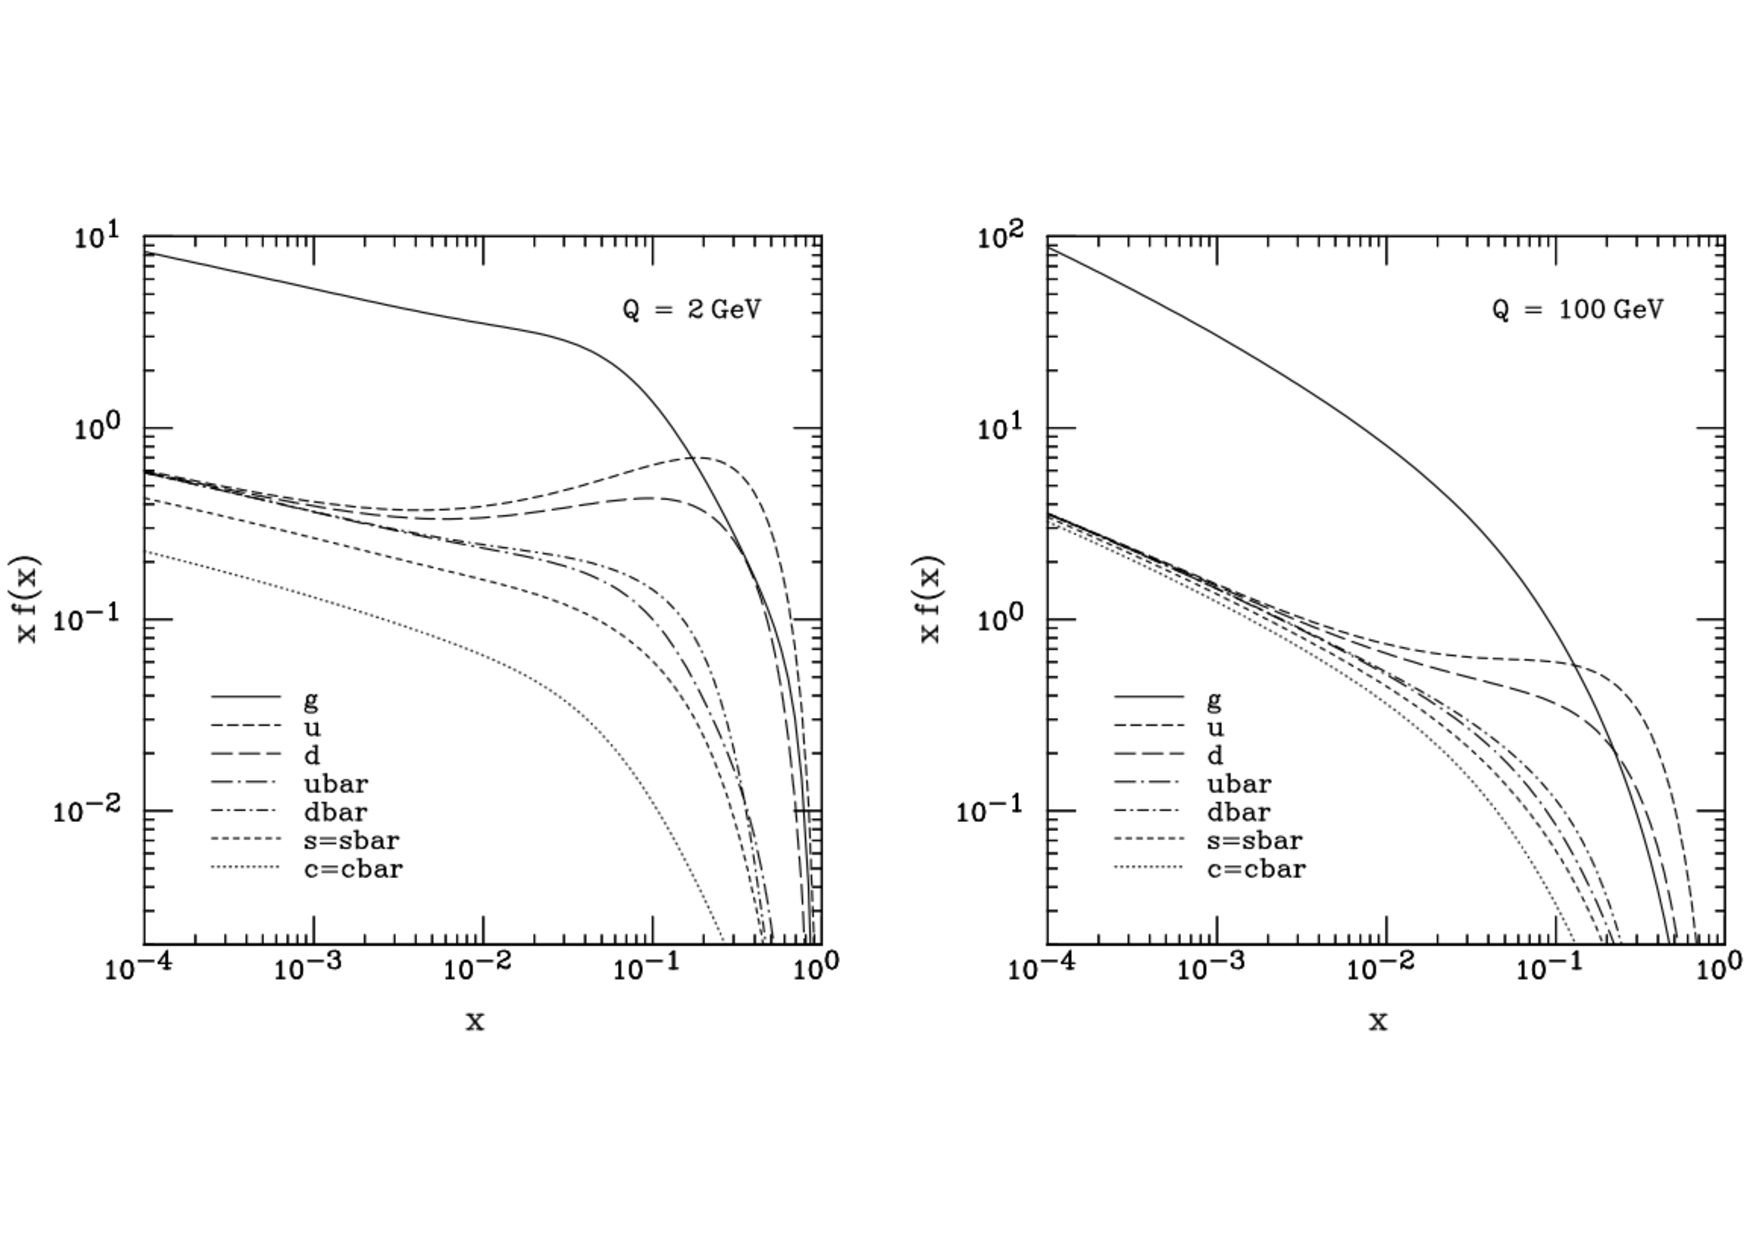
\includegraphics[width=0.6\textwidth]{/Users/rhombus/CMS/Thesis/thesis/pdfs/experiment/cteq_pdf.pdf}
    \label{fig:cteqpdfs}
\end{figure}
%%%%%%%%%%%%%

 Radiation is also important to correctly model.
 At any point in the collision
  any colored particle can radiate a gluon,
  and any charged particle can radiate a photon.
 Gluon radiation from initial state partons is always present
  in $pp$ collisions at the LHC
  and results in jets, columnated showers
  of particles which are the products of quark hadronization
  and gluon splitting.
 The effects of radiation and parton showering are simulated
  using a Markov process in which 
  vertices iteritively are added to partons
  with probabilities based on the
  coupling strengths, energies of the participants
  and the generation of random numbers.
 For the constituents of the proton which
  did not participate in the hard interaction,
  quarks must be created from the vacuum
  to enforce confinement.
 This produces low energy, soft, radiation
  and is known as the underlying event.
 The underlying event must be simulated
  along with the hadronization effects for
  all colored particles.

\subsection{Monte Carlo Generators}
 The two primary generators used in this
  thesis are MadGraph/MadEvent and Pythia.
 MadGraph is strictly a ME generator
  which interfaces with MadEvent for
  event generation
  and Pythia is mostly used for hadronization 
  and showering.
  
 For a given $2\rightarrow n'$
  scattering process, the differential cross section is
  a function of the Lorentz-invariant phase space
  as in Equation~\ref{eq:dsigma}.
 To calculate the cross section within 
  a finite phase space, $d\sigma$
  is integrated and 
  MadGraph numerically does this
  through the sampling of random numbers.
 The phase space can be interpreted as a multidimensional 
  hypercube spanning all degrees of freedom
  for all final state particles
  and Equation~\ref{eq:dsigma} is used
  to calculate a weight, $dw$, for each point
  sampled in the phase space.
 The average
  of the weights converges towards $\int dw$.

 To produce events with the frequency
  predicted by the theory being modeled,
  MadEvent uses the Von Neumann method to unweight events.
 For each event, a random number, $g$, is generated 
  between 0 and 1 and compared to the ratio
  $dw/dw_{\mathrm{max}}$ where $dw_{\mathrm{max}}$
  is the largest event weight sampled.
 If $dw/dw_{\mathrm{max}}>g$ then the event is kept
  and is otherwise rejected.
 Accepted events generated with MadGraph/MadEvent in this 
  way have the same frequency and follow the same
  kinematic distributions as predicted
  from the input Equation~\ref{eq:dsigma}.

 Pythia performs hadronization using the
  Lund string model in which quarks are
  confined to the ends of strings and
  gluons are represented as kinks on that string.
 As quarks separate, the string breaks and
  creates a $q\overline{q}$ pair, 
  thus building confinement directly into the model.
 The underlying event is modeled in Pythia
  as a set of $2\rightarrow 2$ processes
  which are correlated with each other via the
  color connections present in the proton, 
  and the set of parameters used by Pythia
  to perform calculations is referred to as 
  the tune.
 
 % \subsection{MadGraph}
 % \subsection{Pythia}
 % \subsection{MCFM}
 % \subsection{Powheg}
 % \subsection{FEWZ}
 % \subsection{aMC@NLO}

\subsection{Detector Simulation}

 After events have been produced,
  they are passed to Geant4 
  for simulation of the passage of particles
  through the physical mass of CMS.
 The Geant4 toolkit includes a full
  model of CMS, including 
  all of the subdetectors as well as the
  inert material from the support structure
  and readout electronics.
 The magnetic field is emulated using
  data from measurements on the real field
  and Geant4 uses all of this information
  to register hits in the simulated
  detector as a consequence of the interaction
  between particles produced in the simulated
  event and the simulated material of CMS.
 Additionally, hits are added to the
  simulated detector taking into account
  the rates of background noise, and the
  final output is emulated data
  which is stored in the same way
  as would be data as taken from the real detector.



\section{Reconstruction of Events}\label{sec:reconstruction}

 Real data collected from the detector
  and simulated data output from Geant4
  consist of time-correlated energy deposits
  in the various subdetectors of CMS.
 As a result of the coordinated designs 
  of the subdetectors, the final-state 
  particles which arise from $pp$ collisions 
  at the LHC can be individually identified
  and reconstructed using the combined
  information from the entirity of CMS.
 The associated global event description
  from this particle-flow (PF) reconstruction
  provides excellent performance for
  the identification of electrons and muons,
  as well as for vertex identification
  and the evaluation of \met.
 
\subsection{Track and Primary Vertex Reconstruction}
 The subdetector closest to the interaction vertex
  is the tracker, which records precise
  information about the trajectories of 
  charged particles as they pass through it.
 Combined with the magnetic field, 
  this allows for the measurement of the
  momenta of these particles as well as a
  means of identifying the the location of
  the primary interaction.

 Tracks are identified via an iteritive process. 
 The first tracks to be reconstructed
  are those which pass strict seeding
  criteria, designed to have a moderate
  efficiency, but negligibly small
  fake rate.
 Then the detector hits associated
  with these tracks are masked
  and the remaining hits are used to
  form track seeds with slightly relaxed
  criteria.
 This operation is repeated, with every
  iteration imposing more complex and time-consuming
  seeding, filtering and track fitting algorithms.
 
% In 2012, the average number of interactions
%  happening at every bunch crossing was 21,
%  and in 2015 it was 
 Because bunches of protons instead of single protons
  are made to cross in the LHC, 
  multiple collisions can take place during the same
  bunch crossing.
 The vertex with the highest scalar sum
  transverse momentum, \pt,
  of tracks and passing further quality selections
  based on the goodness of fit for the tracks
  and the number of tracks associated with a given vertex
  is chosen as the primary vertex (PV).

 In \ppwbblnbb events, the two $b$ quarks and
  the lepton from the $W$ decay all leave energy
  deposits in the tracker, thus making the choice
  of PV unambiguous.
 However, in the \pploneg events,
  the only visible final state object is a photon,
  and photons do not leave hits in the tracker.
 This makes the identification of the PV
  in the monophoton analysis difficult
  and motivates the using of variables that
  are less sensitive to correct PV identification.
  
\subsection{Electron ID and Reconstruction}

 Electrons are reconstructed using tracker
  hits and ECAL deposits.
 The seed of an electron candidate is selected as 
  an energy deposit in the ECAL with $E_T > 4$ \GeV
  having nearby deposits in the tracker.
 As electrons move in magnetic fields,
  they emit bremsstrahlung radiation
  tangental to their flight path
  and this radiation both appears in the detector, 
  and alters the course of the electron.

 The effects of this radiation are taken
  into account via the Gaussian Sum Filter (GSF)
  track fitting algorithm.
 This algorithm uses weighted sums of Gaussian
  functions to describe electron energy loss
  and thus allows for non-Gaussian corrections
  to the fitting of tracks.
 In the CMS detector, 
  bremsstrahlung from electrons results in the
  emmision of photons in an extended strip
  in the $\phi$ direction and electron
  superclusters (SCs) are made by 
  including the energy deposits from 
  these photons in the ECAL as part of the
  candidate electron object.

 Further requirements during the reconstruction of
  the electron improve the purity of selection.
 The SC and the GSF track are required to 
  be separated by no more than $\abs{\eta}<0.02$
  and $\abs{\phi}<0.15$ and the fraction of
  energy deposited in the HCAL directly behind
  the SC, and the SC is required to be no more
  than 15\%.
 

\subsection{Photon ID and Reconstruction}

 Photons are reconstructed using the same ECAL
  clustering algorithms as are used for electrons.
 This allows for
  the simultaneous reconstruction of
  photons that have and have not split to $e\overline{e}$
  pairs.
 The size of the SC is determined dynamically
  and the center is determined to be the barycenter
  of the distribution, with weights assigned
  using the logarithm of the fractional energy deposits
  of the ECAL crystals clustered in the SC.

 In an ideal tracker, photons would not interact 
  at all and objects that leave signarues
  similar to those of photons could be rejected
  through the rejection of tracks.
 However, some photons do convert to $e\overline{e}$
  pairs inside the tracker volume which leave tracks,
  so the rejection of tracks is not a perfect way 
  to distinguish between photons and electrons.

\subsection{Muon ID and Reconstruction}

 Muon identification is performed using
  two reconstruction and filtering methods to produce 
  `tracker muons' and `standalone muons' which are 
  combined to form  `global muons.'
 Tracker muons are identified starting with
  a track, $\pt>0.5$ \GeV and $p>2.5$ \GeV,
  which is then extrapolated to the muon system.
 If the distance between the the extrapolated
  track and the nearest hit in one of the muon 
  chambers is less than 3 cm, a tracker muon
  is identified.
 Tracker muons are also identified if the 
  pull between the extrapolated track and the
  matched station hit is less than four, where
  pull is defined as the distance between
  the track and the station hit divided by 
  the uncertainties on both measured quanties.
 Tracker muons are built from the inside of the
  detector towards the outside, and 
  standalone muons are built in the other direction.
 Only hits in the muon stations are used to 
  reconstruct standalone muons, with the 
  additional constraint that the path reconstructed
  from the hits points back toward the 
  interaction region.
 Thus, the tracker muon algorithm is well-suited
  for the identification of low-\pt muons by having
  low thresholds and requiring only one track
  and one station hit, while the standalone
  muon algorithm is aimed at high-\pt muons
  which have the energy to penetrate multiple layers
  of muon stations to form tracks which can be
  traced back to the interaction.
 Global muons are required to pass the criteria for both 
  standalone muons and tracker muons, and,
  starting with the standalone muons, 
  the global muon trajectory is refit using information from both 
  the muon stations and the tracker,
  yielding an improved energy resolution than either one.
 %For muons with $\pt<200$ \GeV, the resolution of the tracker




%\subsection{Missing Transverse Energy}

\subsection{Jet ID and Secondary Vertices}
 The reconstruction
  of jets is accomplished using the anti-$k_t$
  clustering algorithm on particles identified 
  in the PF.
 The anti-$k_t$ algorithm is both infrared and collinear
  safe, meaning that it is stable against 
  soft (low energy) radiation getting clustered into individual jets, and 
  also stable against hard (high energy) jets splitting
  collinearly and affecting the shape of the jet.
 
 Jets are corrected in simulation and in data to remove
  energy believed to come from elsewhere than the PV,
  thus removing the luminosity dependence of the jet.
 Jets are also corrected to have a response that is
  independent of $\eta$ by studying dijet events
  and calibrating the jets to anti-align.
 To make the jet response independent of the $\pt$
  of the jet, an absolute correction is applied,
  and in data, one further correction on the relative
  energy scale is applied.
 After all of these corrections are applied, 
  simulated jets are observed to have
  sharper energy resolution than is observed,
  so jets in MC smeared in energy

 Bottom quarks have a relatively long lifetime 
  and are the heaviest fundamental particle
  that has be seen to decay inside the volume of the CMS detector.
 A $b$ quark produced in a $pp$ collision at CMS
  therefore has enough time to hadronize into a jet before
  decaying, and such jets are called $b$-jets.
 The identification, or tagging, of $b$-jets is focused around
  the vertex associated with the $b$-hadron which,
  since it is not the PV but is still a vertex associated
  with the event, is called a secondary vertex, SV.
 The tagging of $b$-jets is accomplished using a multivariate
  analysis technique in which information from variables
  such as the number and energy of tracks that appear to
  be displaced from the PV, the presence of SVs or of
  soft leptons is all combined into a single discriminator value.
  
 
%  for an unstable particle, 
%of 1.5 ps,
%  they decay after about 450 $\mu$m

%%
\chapter{Event Reconstruction}\label{sec:reconstruction}

 Real data collected from the detector
  and simulated data output from Geant4
  consist of time-correlated energy deposits
  in the various subdetectors of CMS.
 As a result of the coordinated designs 
  of the subdetectors, the final-state 
  particles which arise from $pp$ collisions 
  at the LHC can be individually identified
  and reconstructed using the combined
  information from the entirity of CMS.
 The associated global event description
  from this particle-flow (PF) reconstruction
  provides excellent performance for
  the identification of electrons and muons,
  as well as for vertex identification
  and the evaluation of \met.
 
\section{Track and Primary Vertex Reconstruction}
 The subdetector closest to the interaction vertex
  is the tracker, which records precise
  information about the trajectories of 
  charged particles as they pass through it.
 Combined with the magnetic field, 
  this allows for the measurement of the
  momenta of these particles as well as a
  means of identifying the the location of
  the primary interaction.

 Tracks are identified via an iteritive process. 
 The first tracks to be reconstructed
  are those which pass strict seeding
  criteria, designed to have a moderate
  efficiency, but negligibly small
  fake rate.
 Then the detector hits associated
  with these tracks are masked
  and the remaining hits are used to
  form track seeds with slightly relaxed
  criteria.
 This operation is repeated, with every
  iteration imposing more complex and time-consuming
  seeding, filtering and track fitting algorithms.
 
% In 2012, the average number of interactions
%  happening at every bunch crossing was 21,
%  and in 2015 it was 
 Because bunches of protons instead of single protons
  are made to cross in the LHC, 
  multiple collisions can take place during the same
  bunch crossing.
 The vertex with the highest scalar sum
  transverse momentum, \pt,
  of tracks and passing further quality selections
  based on the goodness of fit for the tracks
  and the number of tracks associated with a given vertex
  is chosen as the primary vertex (PV).

 In \ppwbblnbb events, the two $b$ quarks and
  the lepton from the $W$ decay all leave energy
  deposits in the tracker, thus making the choice
  of PV unambiguous.
 However, in the \pploneg events,
  the only visible final state object is a photon,
  and photons do not leave hits in the tracker.
 This makes the identification of the PV
  in the monophoton analysis difficult
  and motivates the using of variables that
  are less sensitive to correct PV identification.
  
\section{Electron ID and Reconstruction}

 Electrons are reconstructed using tracker
  hits and ECAL deposits.
 The seed of an electron candidate is selected as 
  an energy deposit in the ECAL with $E_T > 4$ \GeV
  having nearby deposits in the tracker.
 As electrons move in magnetic fields,
  they emit bremsstrahlung radiation
  tangental to their flight path
  and this radiation both appears in the detector, 
  and alters the course of the electron.

 The effects of this radiation are taken
  into account via the Gaussian Sum Filter (GSF)
  track fitting algorithm.
 This algorithm uses weighted sums of Gaussian
  functions to describe electron energy loss
  and thus allows for non-Gaussian corrections
  to the fitting of tracks.
 In the CMS detector, 
  bremsstrahlung from electrons results in the
  emmision of photons in an extended strip
  in the $\phi$ direction and electron
  superclusters (SCs) are made by 
  including the energy deposits from 
  these photons in the ECAL as part of the
  candidate electron object.

 Further requirements during the reconstruction of
  the electron improve the purity of selection.
 The SC and the GSF track are required to 
  be separated by no more than $\abs{\eta}<0.02$
  and $\abs{\phi}<0.15$ and the fraction of
  energy deposited in the HCAL directly behind
  the SC, and the SC is required to be no more
  than 15\%.
 

\section{Photon ID and Reconstruction}

 Photons are reconstructed using the same ECAL
  clustering algorithms as are used for electrons.
 This allows for
  the simultaneous reconstruction of
  photons that have and have not split to $e\overline{e}$
  pairs.
 The size of the SC is determined dynamically
  and the center is determined to be the barycenter
  of the distribution, with weights assigned
  using the logarithm of the fractional energy deposits
  of the ECAL crystals clustered in the SC.

 In an ideal tracker, photons would not interact 
  at all and objects that leave signarues
  similar to those of photons could be rejected
  through the rejection of tracks.
 However, some photons do convert to $e\overline{e}$
  pairs inside the tracker volume which leave tracks,
  so the rejection of tracks is not a perfect way 
  to distinguish between photons and electrons.

\section{Muon ID and Reconstruction}

 Muon identification is performed using
  two reconstruction and filtering methods to produce 
  `tracker muons' and `standalone muons' which are 
  combined to form  `global muons.'
 Tracker muons are identified starting with
  a track, $\pt>0.5$ \GeV and $p>2.5$ \GeV,
  which is then extrapolated to the muon system.
 If the distance between the the extrapolated
  track and the nearest hit in one of the muon 
  chambers is less than 3 cm, a tracker muon
  is identified.
 Tracker muons are also identified if the 
  pull between the extrapolated track and the
  matched station hit is less than four, where
  pull is defined as the distance between
  the track and the station hit divided by 
  the uncertainties on both measured quanties.
 Tracker muons are built from the inside of the
  detector towards the outside, and 
  standalone muons are built in the other direction.
 Only hits in the muon stations are used to 
  reconstruct standalone muons, with the 
  additional constraint that the path reconstructed
  from the hits points back toward the 
  interaction region.
 Thus, the tracker muon algorithm is well-suited
  for the identification of low-\pt muons by having
  low thresholds and requiring only one track
  and one station hit, while the standalone
  muon algorithm is aimed at high-\pt muons
  which have the energy to penetrate multiple layers
  of muon stations to form tracks which can be
  traced back to the interaction.
 Global muons are required to pass the criteria for both 
  standalone muons and tracker muons, and,
  starting with the standalone muons, 
  the global muon trajectory is refit using information from both 
  the muon stations and the tracker,
  yielding an improved energy resolution than either one.
 %For muons with $\pt<200$ \GeV, the resolution of the tracker




\section{Missing Transverse Energy}

\section{Jet ID and Secondary Vertices}



\chapter{W+bb Cross Section Measurement}\label{sec:wbbxc}

We now have the tools in place to examine the first of the
 two Standard Model (SM) processes investigated in this text.
This process is \ppwbb at \s 8 \TeV with colliding protons
 provided by the Large Hadron Collider and detected
 by the Compact Muon Solenoid experiment. 

\section{Previous Measurements}

The production of \z bosons
 \cite{Chatrchyan:2012vr,Chatrchyan:2014dha,Chatrchyan:2013zja,Aad:2011jn,Aad:2014dvb}
 or \w bosons \cite{Chatrchyan:2013uza,Aad:2013vka}
 in association with b jets has been 
 studied at a center-of-mass
 energy of 7 TeV using data samples with up
 to 5 \fbinv of integrated luminosity,
 by the ATLAS and CMS experiments, 
 as well as at 
 the Tevatron \cite{WbbTevD0,WbbTevCDF} at $\sqrt{s}=1.96$ TeV. 
This analysis extends previous measurements of the \wbb cross section \cite{Chatrchyan:2013uza},
 using data at $\sqrt{s}=8 \TeV$, collected by the CMS detector in 2012 
 and corresponding to an integrated luminosity of 19.8 \fbinv \cite{ref:CMSLumiCalc}.
 %=====expand=======

\section{Event Selection}

 Two decay channels of the \w boson are considered,
  $\w\rightarrow \mu\nu_\mu$ and $\w\rightarrow e\nu_e$,
 and events are selected using
 single-muon (single-electron) triggers with a
 loosely isolated muon (electron)
 with transverse momentum $\pt>24~(27)$ \GeV
 and pseudo-rapidity $\abs{\eta}<2.1~(2.5)$.
Individual particles emerging from each collision are then reconstructed with the
 particle-flow (PF) technique described in Section \ref{sec:particleflow}
 which ultimately has the effect of dividing them 
 into mutually exclusive categories:
 charged and neutral hadrons, photons, electrons, and muons.

Both the muon and electron candidates are required to have 
 $\pt$ larger than 30 \GeV and $\abs{\eta}<2.1$ and
 to originate from the primary vertex of the event,
 chosen as the vertex with the highest $\sum \pt^2$
 of the charged particles associated with it.
These leptons must additionally pass a tight ID requirement 
 described in Section \ref{sec:leptonid},
 and  must be isolated where
 the isolation variable is defined as

\begin{equation}
\label{eq:iso}
I =\frac{ \sum\pt^{\mathrm{charged}}+{\mathrm{max}}(0,\sum\pt^{\gamma}+\sum\et^{\mathrm{neutral}}-0.5\cdot\pt^{\mathrm{PU}})}{\pt^\ell},
\end{equation}
 with the sum running over the PF candidates (hadrons, electrons, photons)
 in a cone of size $\Delta R < 0.4~(0.3)$ around the muon (electron) direction.
 %where $\Delta R = \sqrt {\smash[b]{ (\Delta \eta)^2 + (\Delta \phi)^2}}$.
The isolation includes a correction for pileup effects,
 which is based on the scalar sum of transverse momenta of charged particles
 not associated with the primary vertex in the isolation cone 
 ($\pt^{\mathrm{PU}}$).
The selected muons (electrons) are required to
 have $I < 0.12~(0.10)$.

Missing transverse energy, $\vmet$, is defined in Section \ref{sec:met}
 as the negative vector sum of the transverse momenta
 of all reconstructed particle candidates in the event.
 It is  combined with the $\pt$ of a muon or electron passing
 the identification and isolation requirements to form a $\w$ candidate.
%Assuming a negligible lepton mass, the transverse mass, $\mt$, of the W is defined as 
%
% \begin{equation}
% \mt^2 = 2 E_T^{\mathrm{miss}} \pt^\ell \left(1-\cos\Delta\phi\right) % massless lepton approximation
% \end{equation}
% where $\Delta\phi$ is the azimuthal angle between the lepton $\vec{\pt}$
% and $\vmet$.
The transverse mass of the \w boson, as defined in Section \ref{sec:transversemass},
  is a  natural discriminator against non-$\w$ final states
 such as QCD multijet events,
 that have a lepton candidate and $\vmet$,
 but a relatively low value of $\mt$.
In calculating \mt, the \met is corrected for noise in the
 electromagnetic and hadron calorimeters \cite{WZCMS:2010}.
 and corrections to mitigate the effect of the
 pileup are also included \cite{CMS:8TeVMET}.

Jets are constructed using the anti-$k_t$ clustering algorithm \cite{Cacciari:2008gp},
 as implemented in the \textsc{fastjet} package \cite{fastjet1,fastjet2},
 with a distance parameter of 0.5.
Jet clustering is performed using individual particle candidates reconstructed with the PF technique.
Jets are required to pass identification
 criteria that eliminate jets originating from
 noisy channels in the hadron calorimeter \cite{Chatrchyan:2009hy}.
Those which originate from pileup interactions are
 rejected by requiring consistency of the jets
 with the primary interaction vertex.
Small corrections to the relative and absolute jet energy calibrations of the detector are
 applied as a function of the $\pt$ and $\eta$  of the jet \cite{cmsJEC}.

The combined secondary vertex (CSV) b-tagging algorithm \cite{CMS-PAS-BTV-13-001,cmsBTAGPAPER} exploits
 the long lifetime and relatively large mass of b hadrons to provide optimized
 b jet discrimination.
The CSV algorithm combines information about impact parameter
 significance, secondary vertex (SV) kinematic properties, and jet kinematic
 properties in a likelihood-ratio technique.
The tagging of a jet is made by imposing a minimum threshold on
 the CSV discriminator value and in this analysis we require
 that both jets pass a threshold which has a b-tagging
 efficiency of about 40\% and a misidentification probability of
 %efficiency of about 50\% and a misidentification probability of
 0.1\% for light jets and 1\% for charm jets.
The scale factors used to correct for the differences in efficiency
 between data and simulation take into account dependencies on
 the transverse momentum of the jet.

After all selection requirements for the signal enhanced dataset are applied,
 the contributing processes to the overall yield are the
 associated production of a massive vector boson and jets ($\vjets$),
 as well as diboson ($\WW$, $\WZ$, $\ZZ$), $\ttbar$, single top, $\gjets$, and QCD multijet production.
The corresponding contributions are estimated from simulation except for QCD, which
 is estimated from data as described in Section \ref{sec:qcd}.
To prove the validity of the MC shapes and normalizations a set of control regions is 
 provided for the background contributions.

\section{Background Estimation}

\subsection{QCD}
\label{sec:qcd}
The QCD multijet sample derived using a data-driven method. 
The shapes of the distributions for QCD multijet events are taken as the difference between
 the data sample and the sum of the other simulated backgrounds in a region of phase
 space enriched in multijets.
The shape of the QCD used in the signal region comes from the distributions 
 illustrated in Fig. \ref{fig:qcdshape}.
This region is found using the same selection requirements as those in the signal region,
 but requiring the muon (electron) to be antiisolated: $I > 0.20 \; (0.15)$.
In the fiducial regions used in this analysis, minimal correlation
 is observed between $I$ and $\mt$, validating
 the use of an inverted isolation requirement to obtain
 the QCD shape.
This shape is then scaled by $ (d_{20}-m_{20})/q_{20} $ where
 $d_{20}$ is the yield in data in the range $0<\mt<20$, $m_{20}$ is the combined
 yield from the simluated samples in this range, and $q_{20}$ is the corresponding
 unnormalized yield of QCD multijet.
This has the effect of normalizing the QCD sample such that the combination of the QCD 
 and the simulated backgrounds has the same total yield as data in the range $0<\mt<20$.
If $d_{20}<m_{20}$, the QCD contribution is taken to be negligable. % and is scaled by $10^{-6}$.
% this happens for ttbar multi-lepton
The relative uncertainty in the yield of QCD multijet events is
 estimated to be $\pm$50\%, taking into account both the fit result
 and the extrapolation from $0<\mt<20$ to the high-$\mt$ range.
This relative uncertainty also covers shape mismodelings
 of the multijet contribution in the final sample.


\begin{figure}
 \caption[QCD shape for \wbb analysis]
 {The shape for the QCD is found by inverting the lepton
  isolation and subtracting MC from the data.
  Shown above is the data, MC background and 
   extrapolated QCD shape (difference between data
   and MC backbrounds) in this inverted
   region for both the muon and electron channels
   in the $W+jj$ and $W+b\bar{b}$ phase spaces.
  The requirement of two well-identified b tags
   essentially eliminates all MC backgrounds in
   the $W+b\bar{b}$ region, leaving the QCD shape 
   the same as that of the data.
  }
 \center
\label{fig:qcd_mu}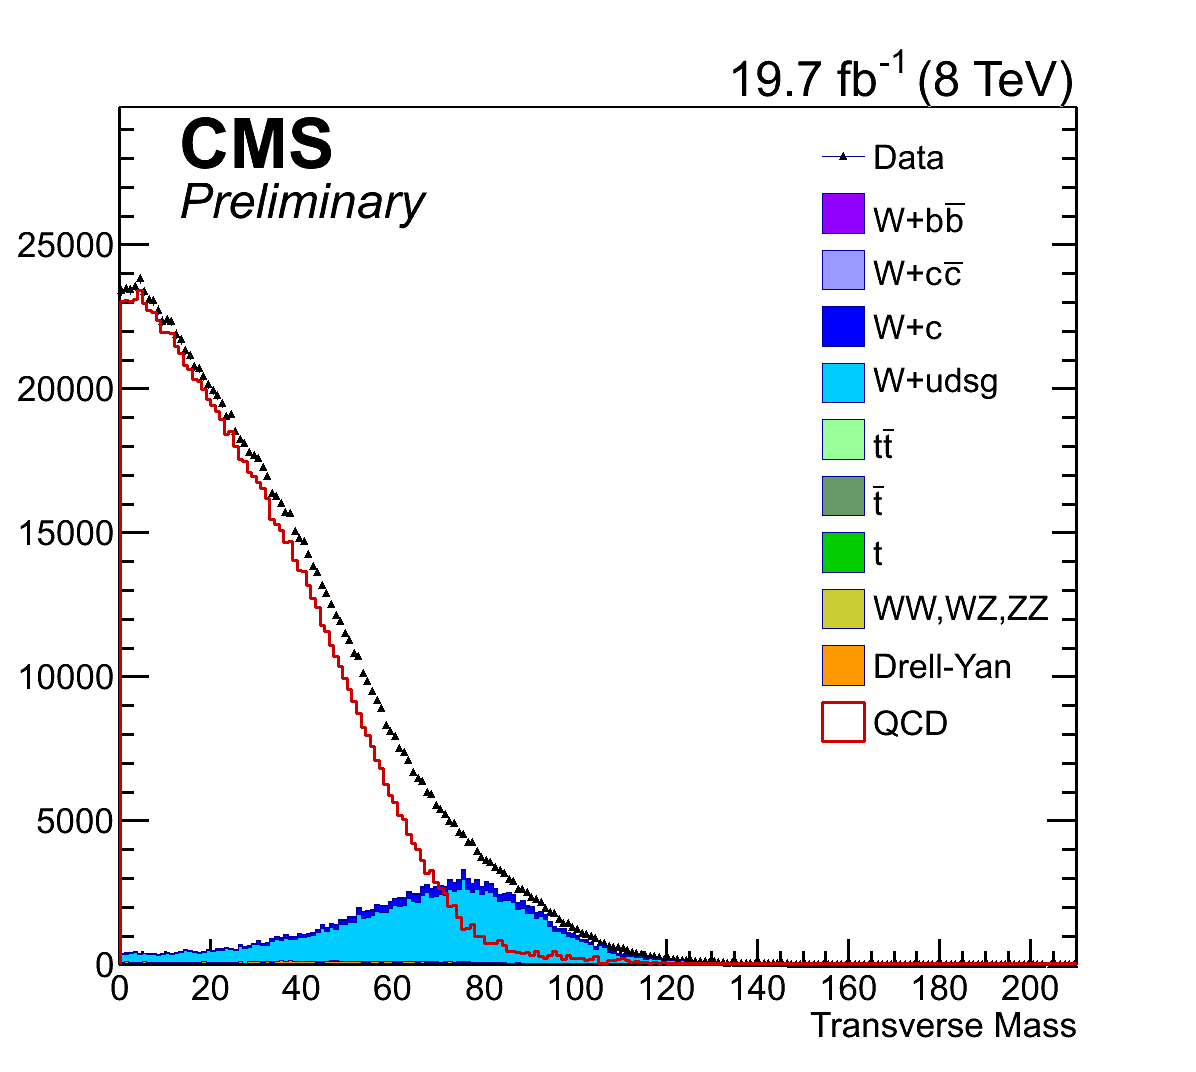
\includegraphics[width=0.4\textwidth]{/Users/rhombus/CMS/Thesis/thesis/pdfs/wbbxc/qcd/QCDShape_wjj_mt_mu.png}
\label{fig:qcd_mu}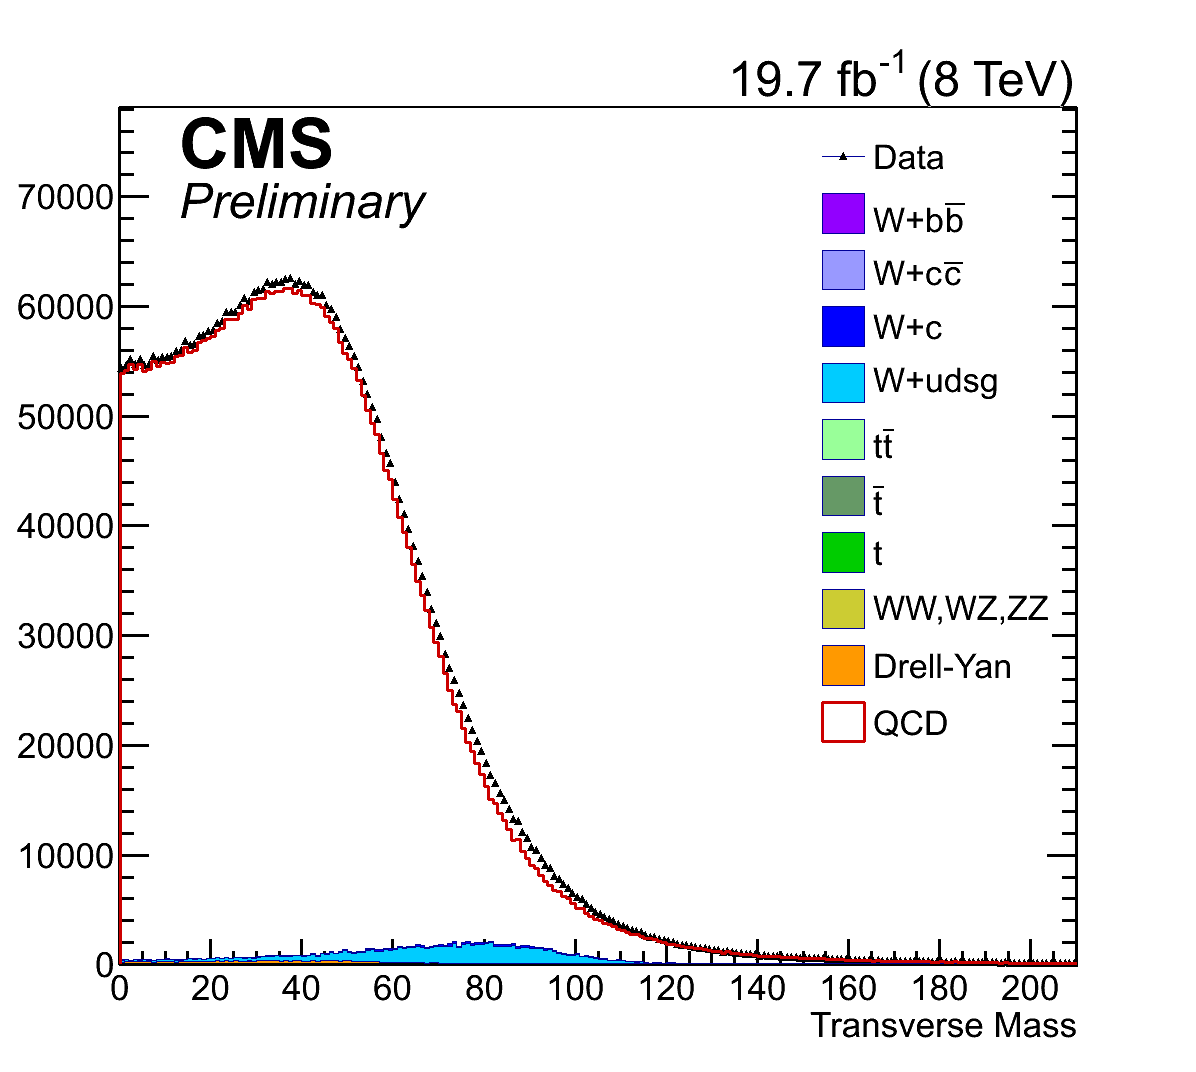
\includegraphics[width=0.4\textwidth]{/Users/rhombus/CMS/Thesis/thesis/pdfs/wbbxc/qcd/QCDShape_wjj_mt_ele.png}
\label{fig:qcd_mu}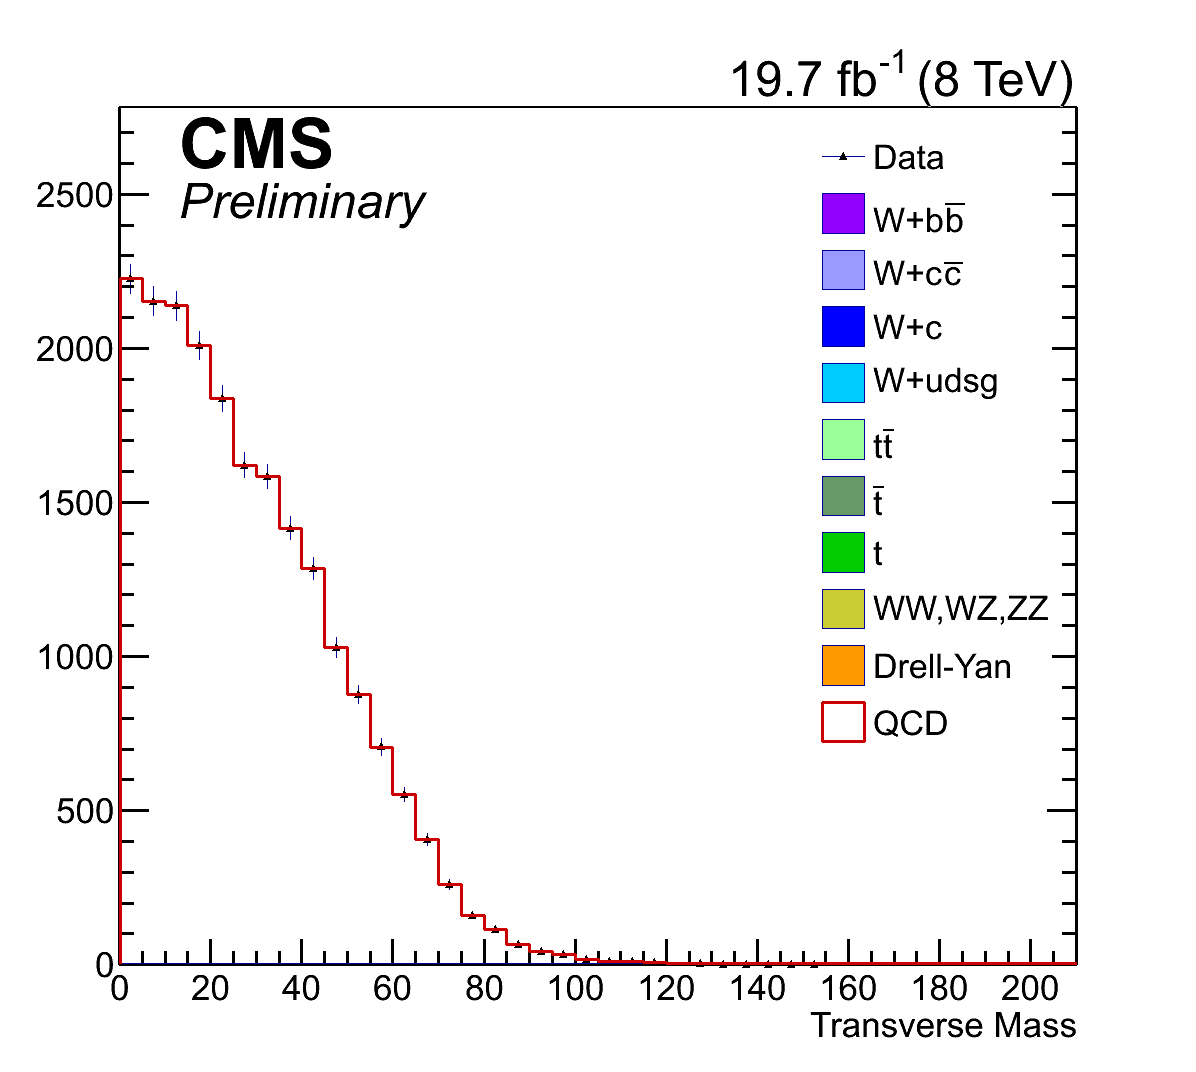
\includegraphics[width=0.4\textwidth]{/Users/rhombus/CMS/Thesis/thesis/pdfs/wbbxc/qcd/QCDShape_wbb_mt_mu_05.png}
\label{fig:qcd_mu}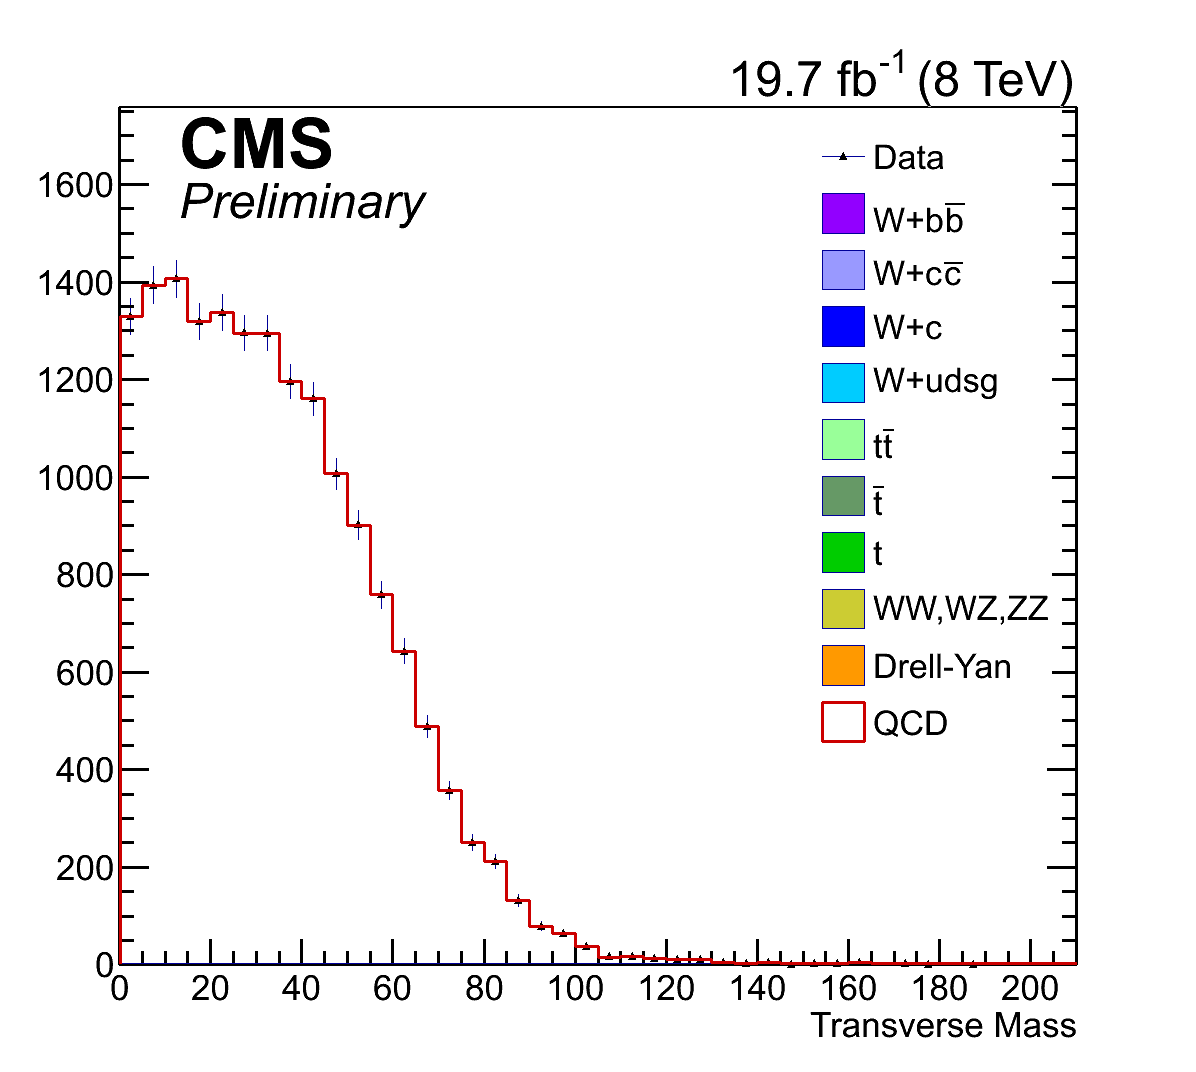
\includegraphics[width=0.4\textwidth]{/Users/rhombus/CMS/Thesis/thesis/pdfs/wbbxc/qcd/QCDShape_wbb_mt_ele_05.png}
 \label{fig:qcdshape}
\end{figure}



\subsection{W+jets: light and charm component}

$W$+jets is the dominating background in the $W+jj$ phase space,
 which is found using idential selections as are used in 
 the signal region with the exception of the b tag requirement;
 in the $W+jj$ phase space, no requirements on b tags are made.
This control region therefore serves as a cross check on the 
 reconstructed objects observed in the signal region before
 the added complication of b tagging has been introduced. 
In Figure~\ref{fig:wjj_plots} is shown the \pt 
 of the identified lepton along with the \met and \mt
 in both decay channels.
Agreement between simulation and data is on the order of 10\%.

\begin{figure}
 \caption[\wjj control region for the \wbb measurement]{
  Selecting for a tight ID muon with $\pt>$30 GeV and exactly two central jets passing loose ID,
   we recover the distributions shown above. 
  Shown in the upper left (right)
   is the momentum of the leading lepton in the muon (electron) channel.
  The missing transverse energy is shown in the center,
  and transverse mass is given in the bottom two distributions.
  The shaded band in ratio plots shows statistical uncertainty. 
 } 
 \center
 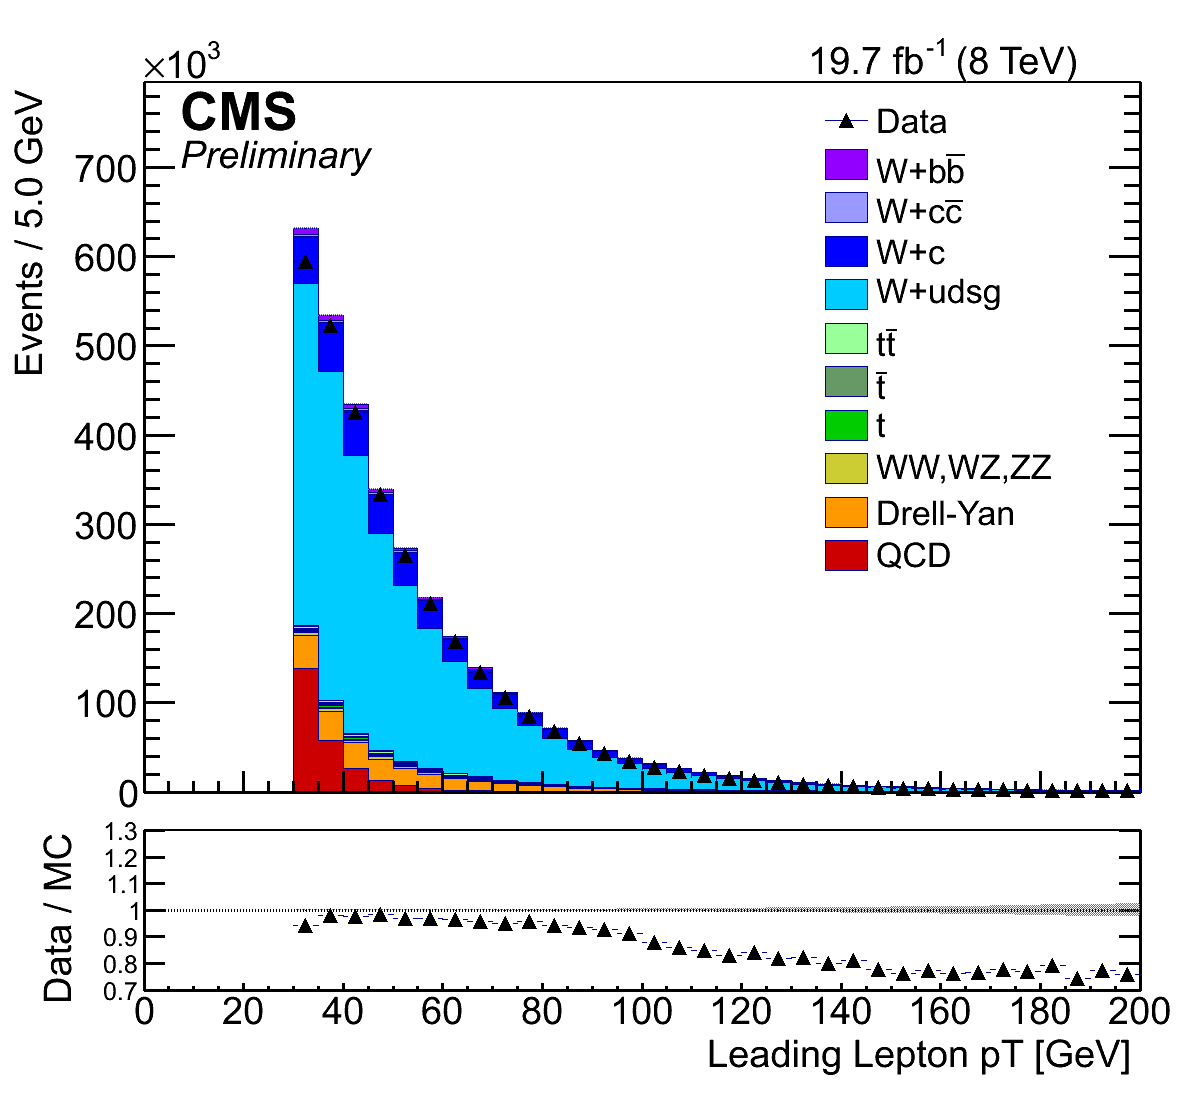
\includegraphics[width=0.4\textwidth]{/Users/rhombus/CMS/Thesis/thesis/pdfs/wbbxc/wjj/Histograms_wjj_goodLep_pt_mu.png}
 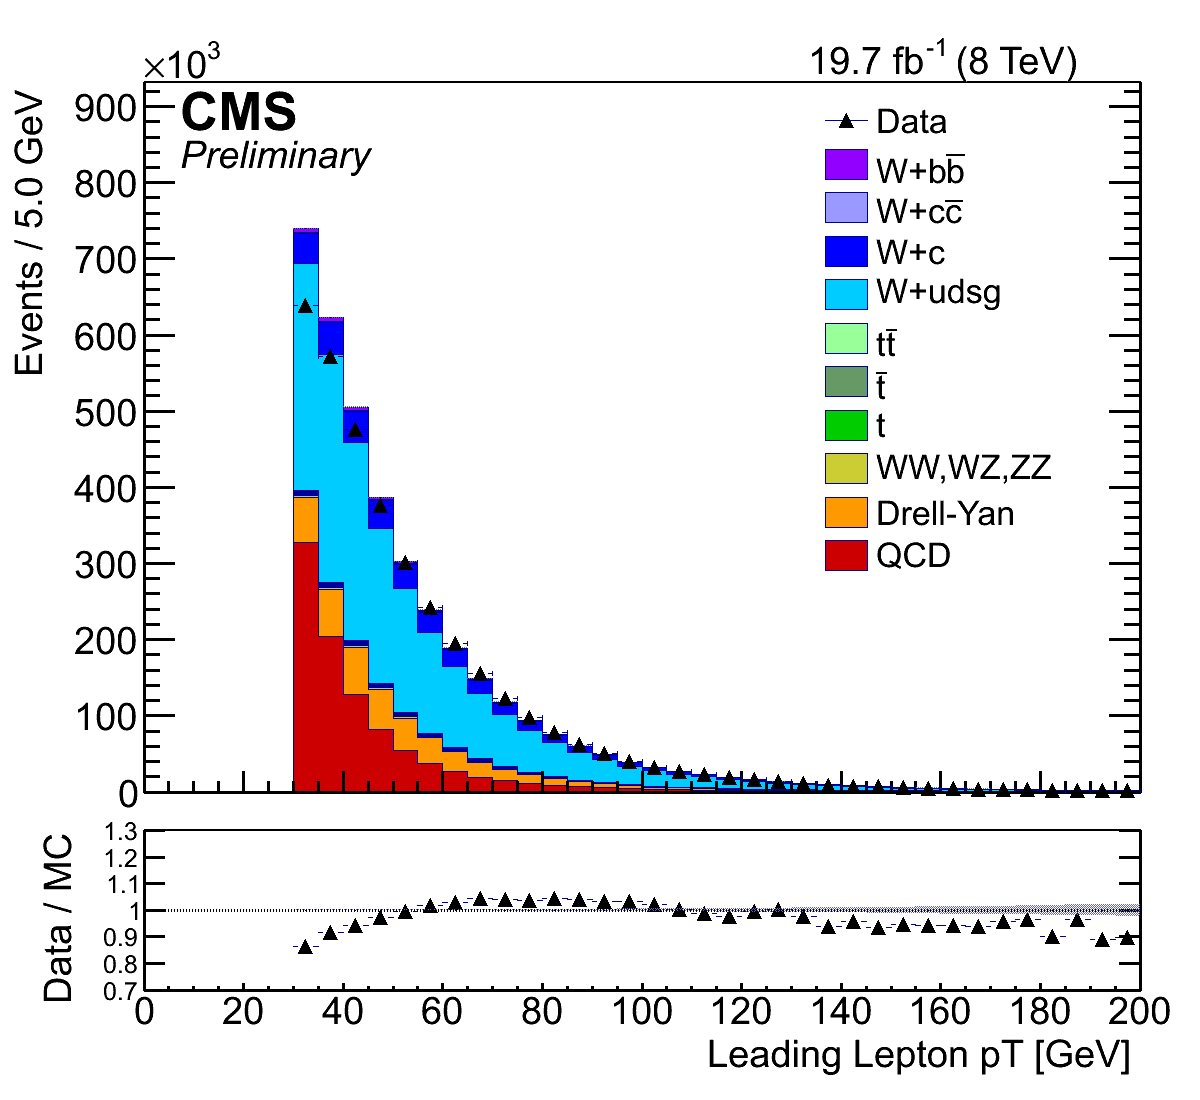
\includegraphics[width=0.4\textwidth]{/Users/rhombus/CMS/Thesis/thesis/pdfs/wbbxc/wjj/Histograms_wjj_goodLep_pt_ele.png}
 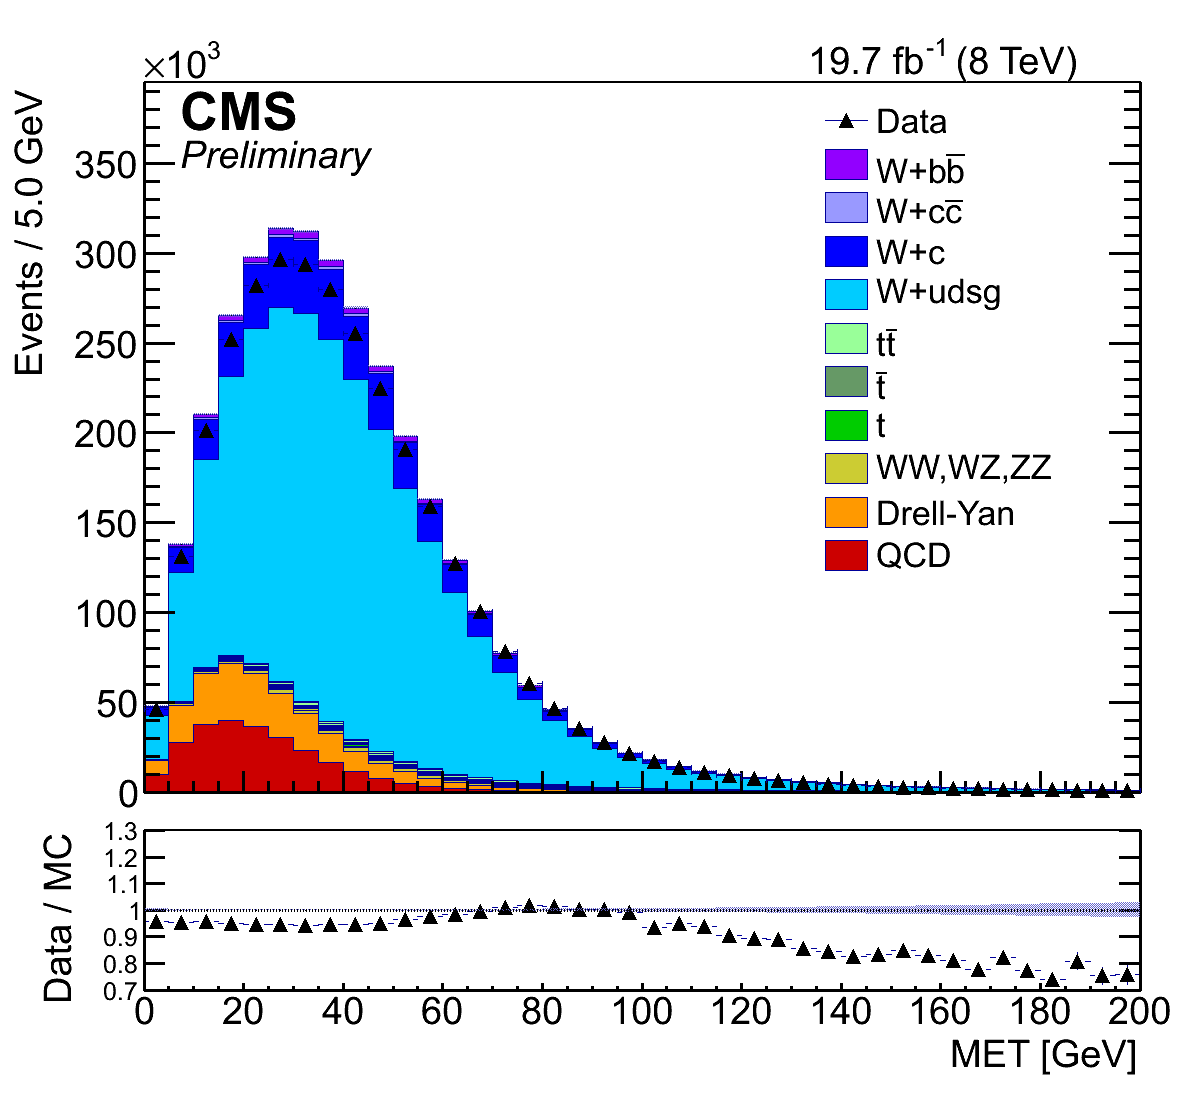
\includegraphics[width=0.4\textwidth]{/Users/rhombus/CMS/Thesis/thesis/pdfs/wbbxc/wjj/Histograms_wjj_met_mu.png}
 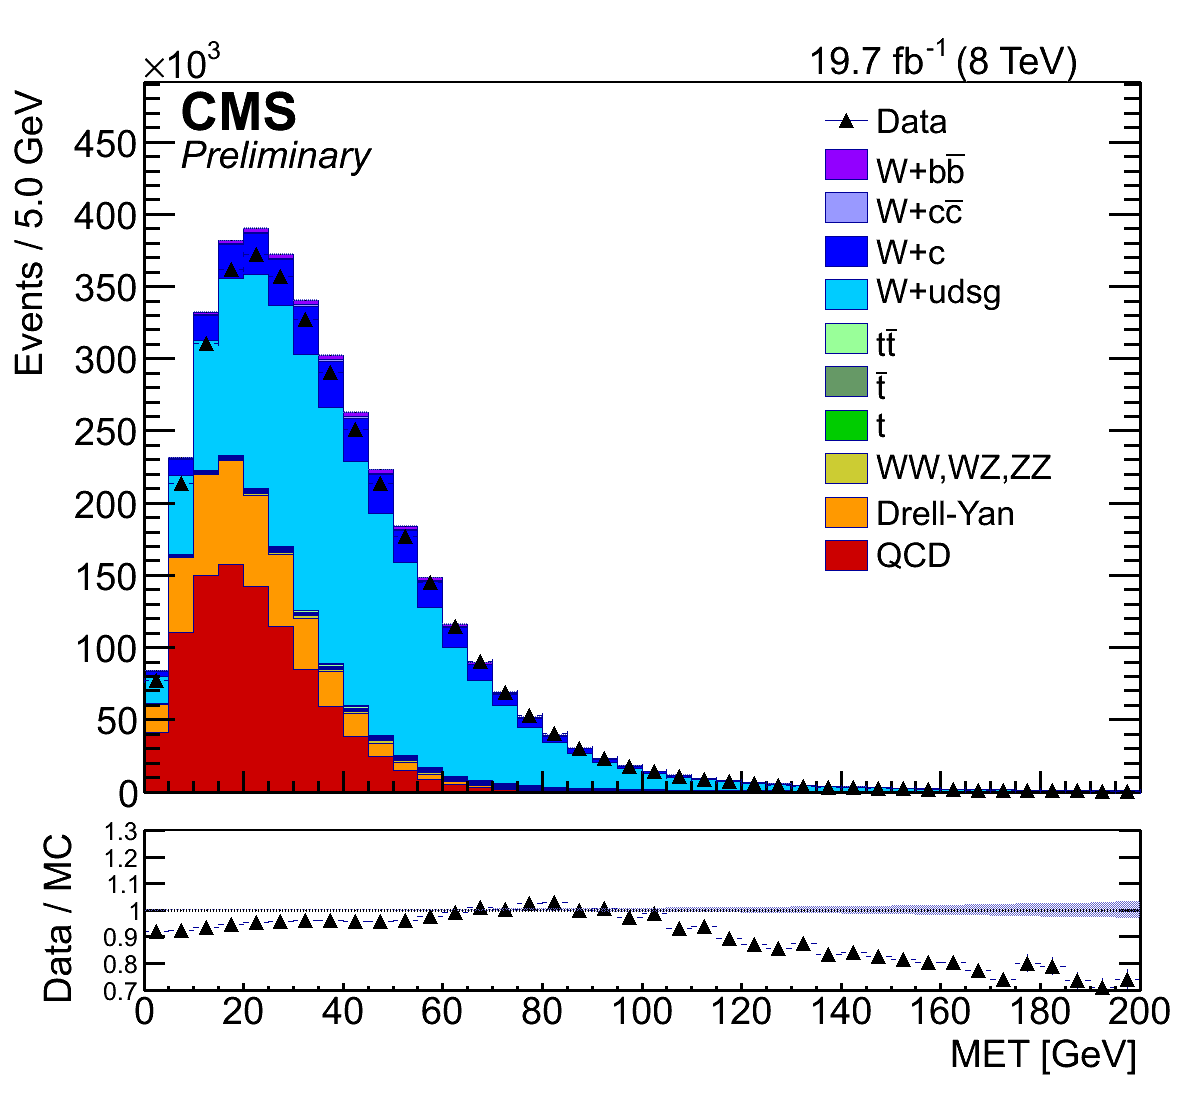
\includegraphics[width=0.4\textwidth]{/Users/rhombus/CMS/Thesis/thesis/pdfs/wbbxc/wjj/Histograms_wjj_met_ele.png}
 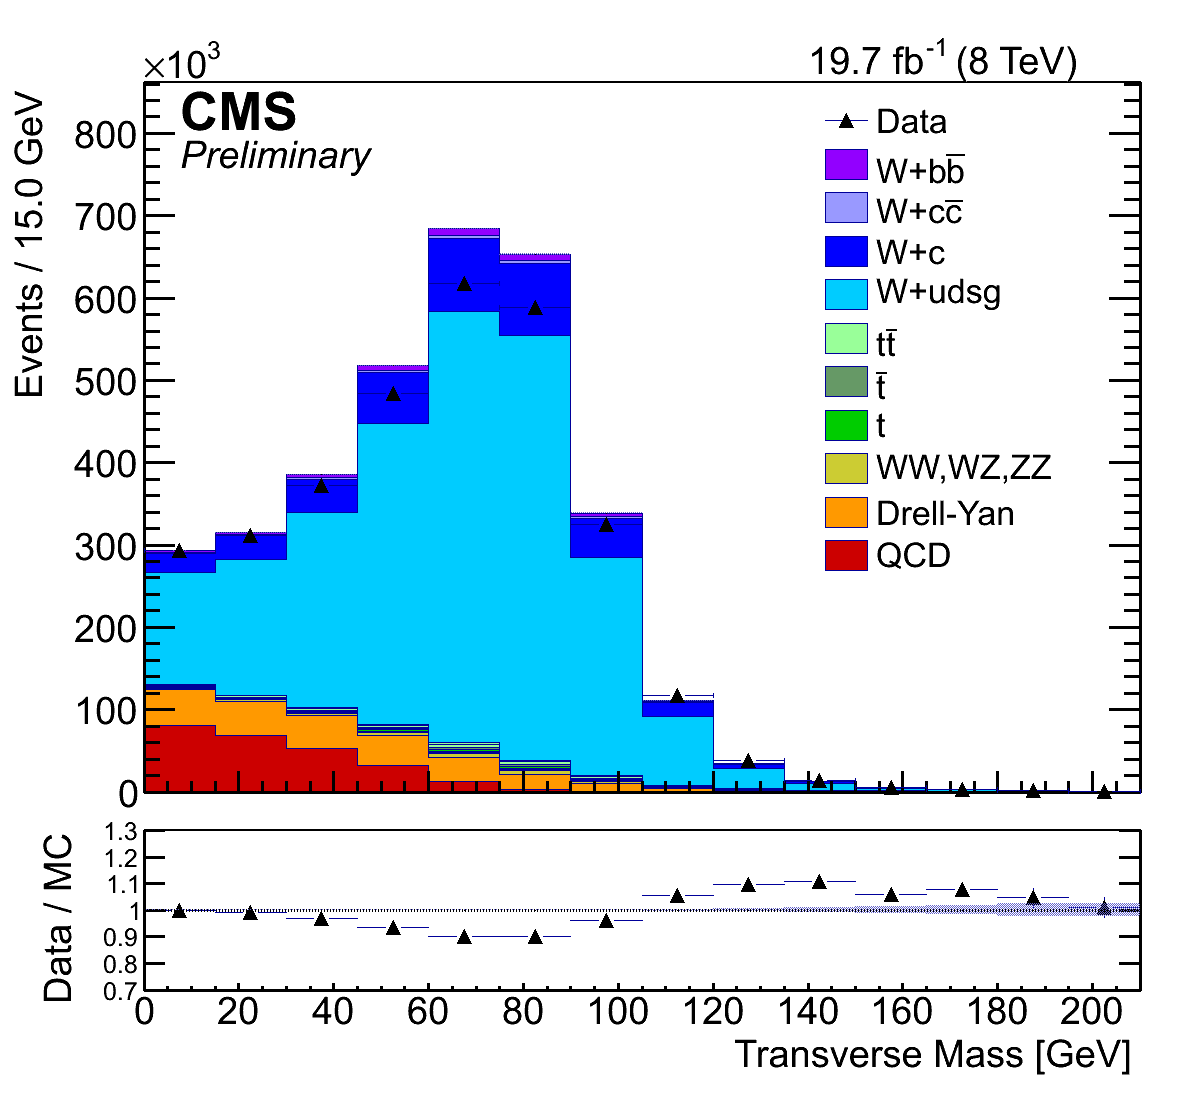
\includegraphics[width=0.4\textwidth]{/Users/rhombus/CMS/Thesis/thesis/pdfs/wbbxc/wjj/Histograms_wjj_mt_mu.png}
 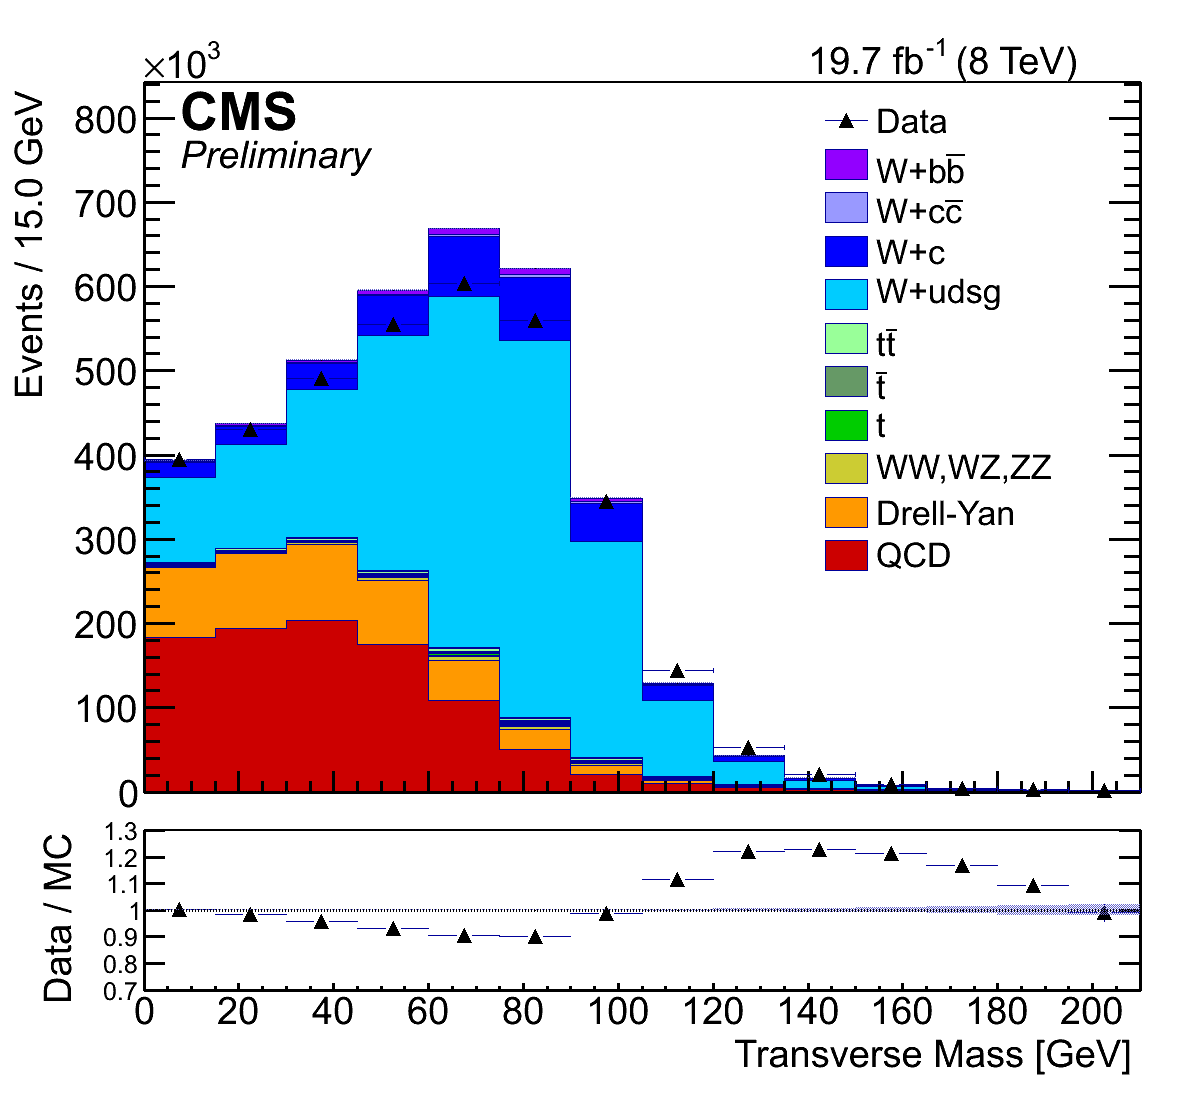
\includegraphics[width=0.4\textwidth]{/Users/rhombus/CMS/Thesis/thesis/pdfs/wbbxc/wjj/Histograms_wjj_mt_ele.png}
    \label{fig:wjj_plots}
\end{figure}

The true $\wc$ contribution in the signal region is minimal, 
and only possible due to mistaging of a second jet in
the event. However, the contribution of events
with one hard charm and one hard anti-charm originated by gluon 
splitting is not negligable and moreover these events have kinematics closely related 
to that of our signal. 

\subsection{Top backgrounds}
\label{section:topbackgrounds}

To validate the description of the $\ttbar$ contribution two 
 control regions are defined and referred to as multilepton 
 and multijet $\ttbar$ regions.
The selections for the multijet region are the same as 
 those for the $\wbb$ region except that additional jet
 activity is required by selecting events with at least
 three jets in the final state. 
Because of the loosening of the jet veto in this phase space,
 it is less sensative to the effects of jet energy scaling
 than the signal region (2\% in the \ttbar multijet phase space,
 6\% in the \wbb phase space.)
As can be seen in Figure \ref{fig:prefit_ttjjj},
 this control region is dominated by $\ttbar$, with $\ttbar$ accounting for
 80\% of the data yield.

\begin{figure}
      \caption[\ttbar-multijet control region for the \wbb measurement]
   {Distributions in the $\ttbar$ multijet control region are shown here in both channels.
       These raw distributions are made before any of the scaling outlined in Section \ref{subsec:wbb_analysisstrategy}.
       Left plots are in the muon decay channel and right
        plots are in the electron decay channel.
      }
      \center
 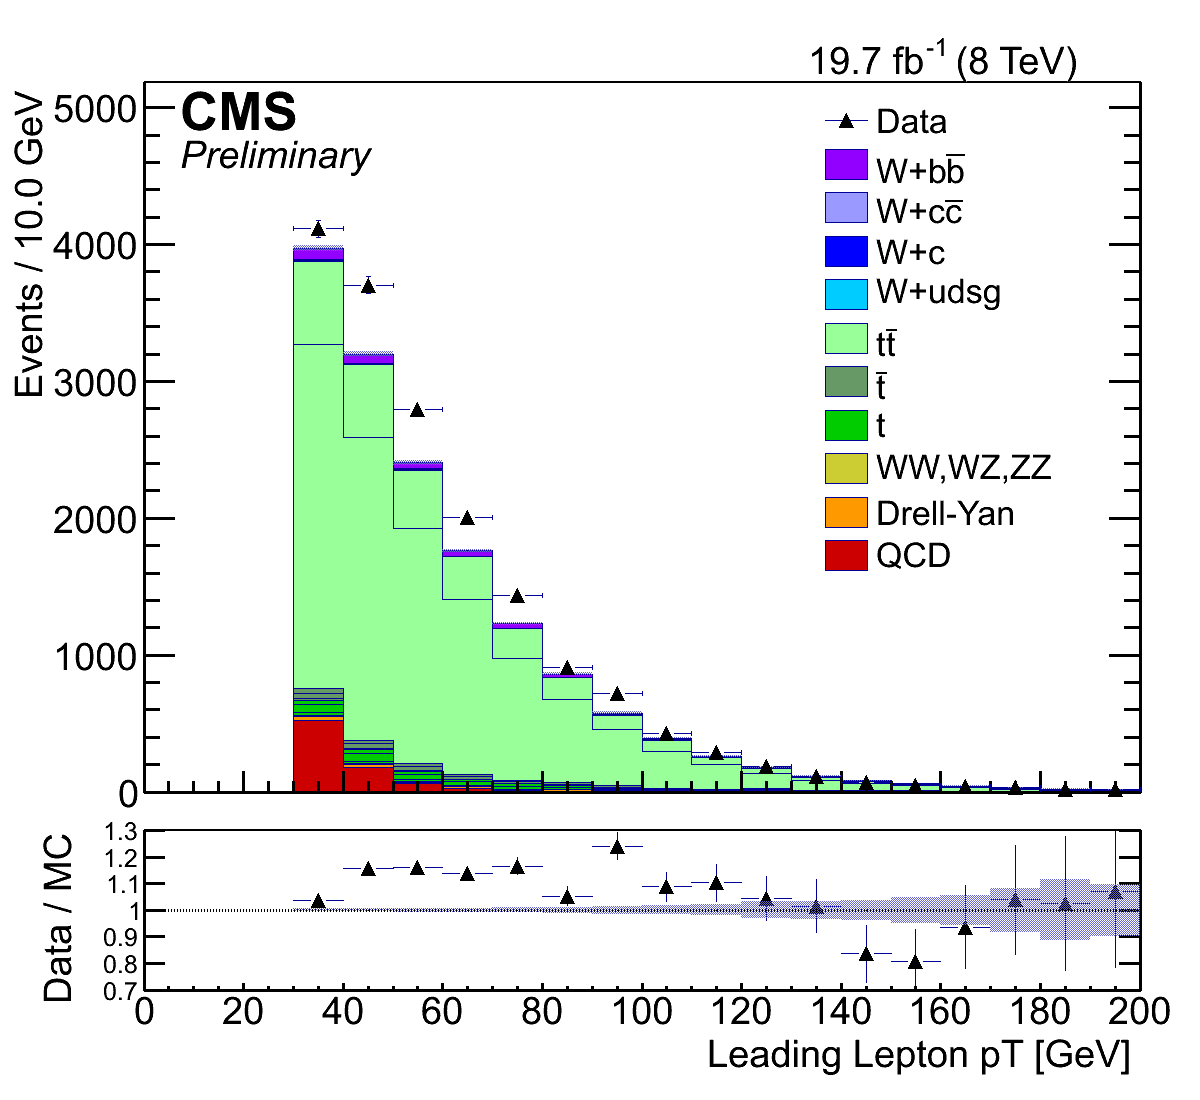
\includegraphics[width=0.4\textwidth]{/Users/rhombus/CMS/Thesis/thesis/pdfs/wbbxc/ttjjj/Histograms_ttjjj_goodLep_pt_mu.png}
 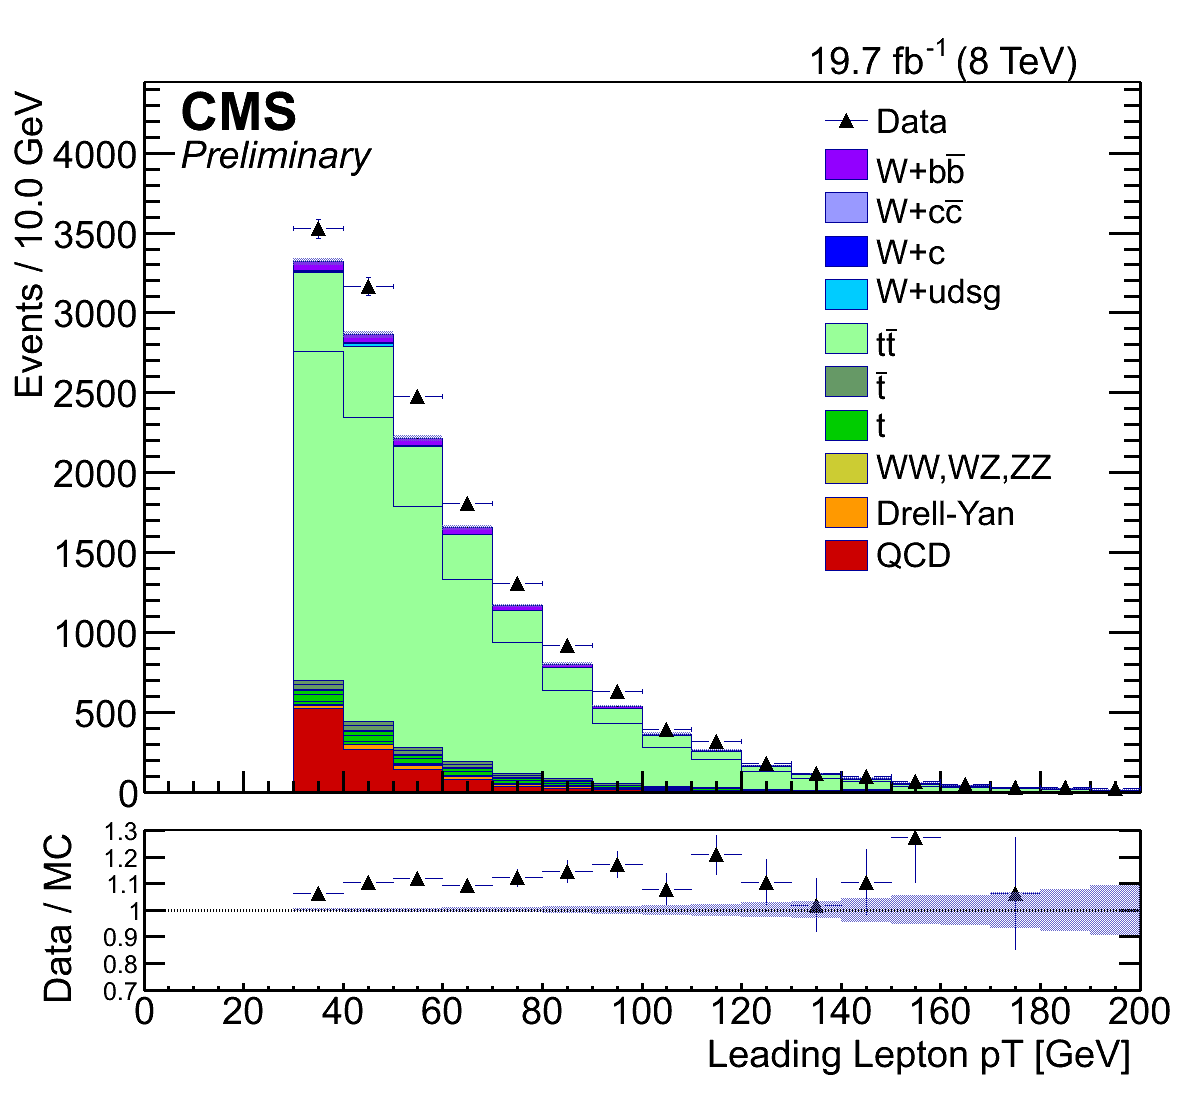
\includegraphics[width=0.4\textwidth]{/Users/rhombus/CMS/Thesis/thesis/pdfs/wbbxc/ttjjj/Histograms_ttjjj_goodLep_pt_ele.png}
 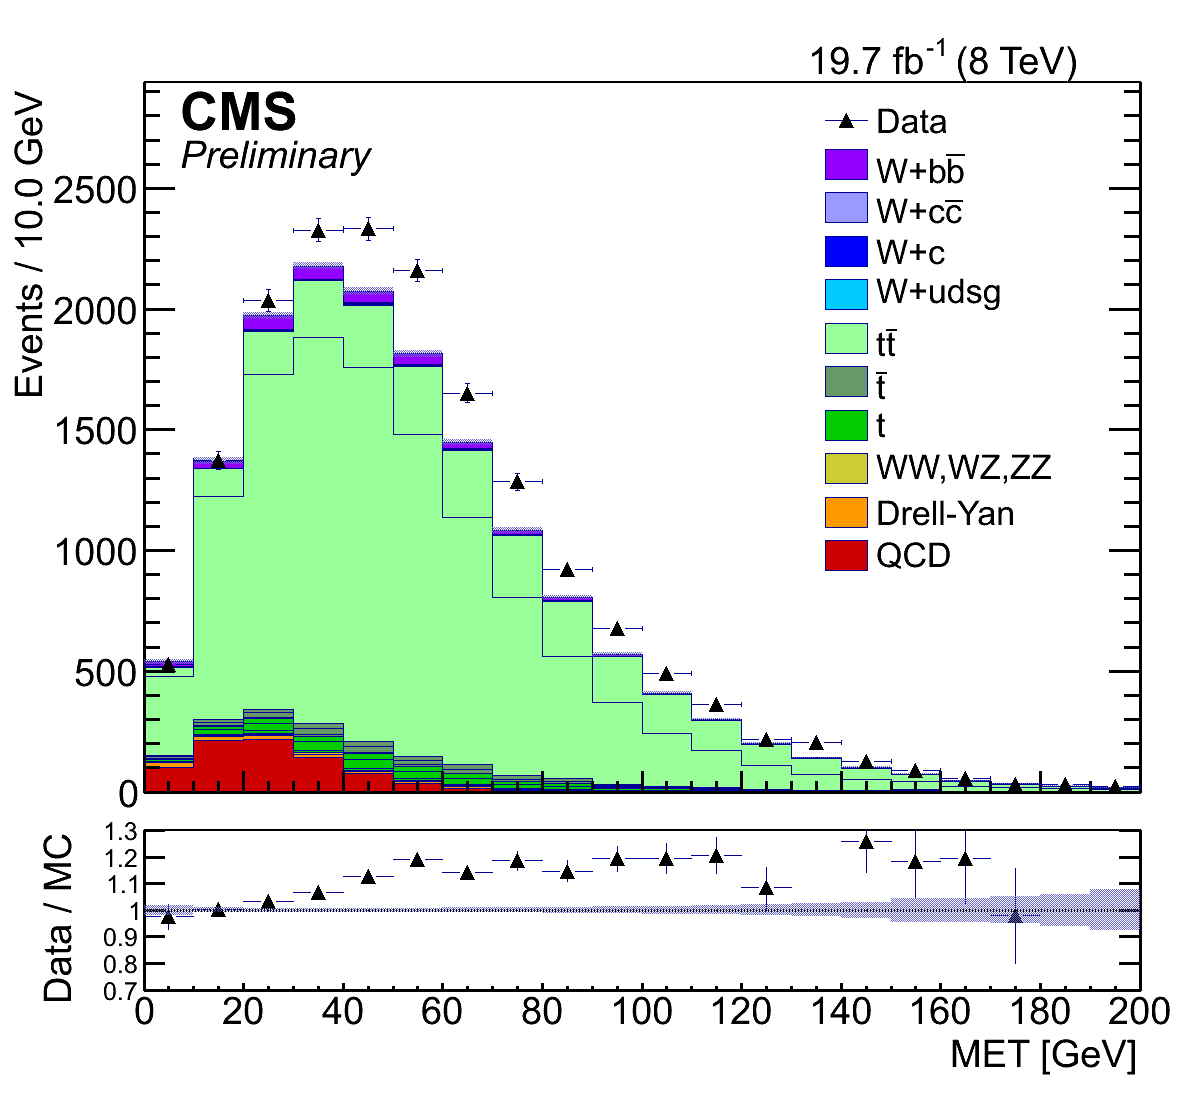
\includegraphics[width=0.4\textwidth]{/Users/rhombus/CMS/Thesis/thesis/pdfs/wbbxc/ttjjj/Histograms_ttjjj_met_mu.png}
 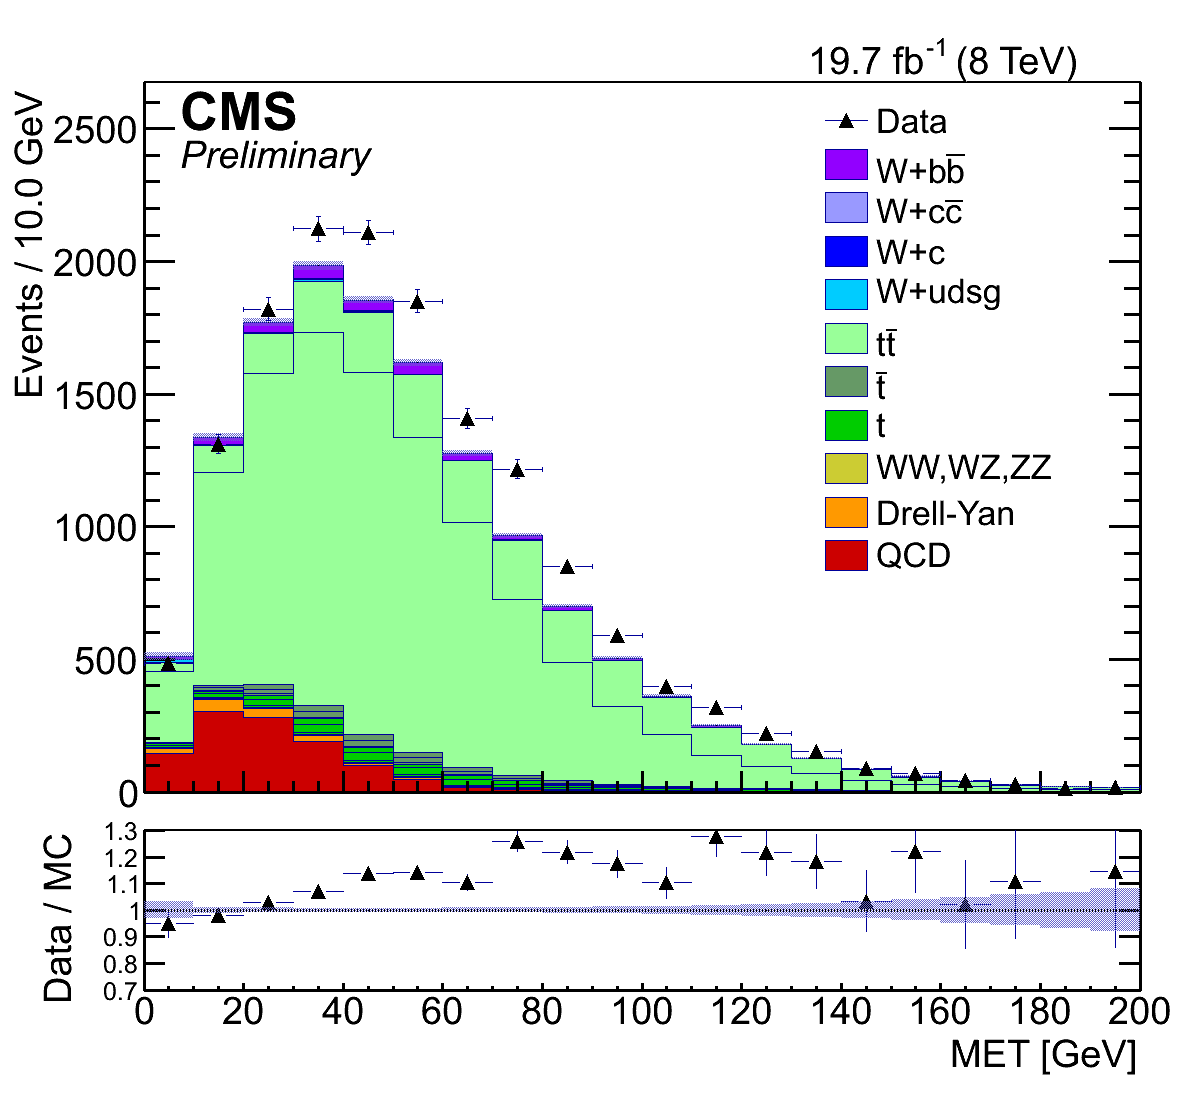
\includegraphics[width=0.4\textwidth]{/Users/rhombus/CMS/Thesis/thesis/pdfs/wbbxc/ttjjj/Histograms_ttjjj_met_ele.png}
 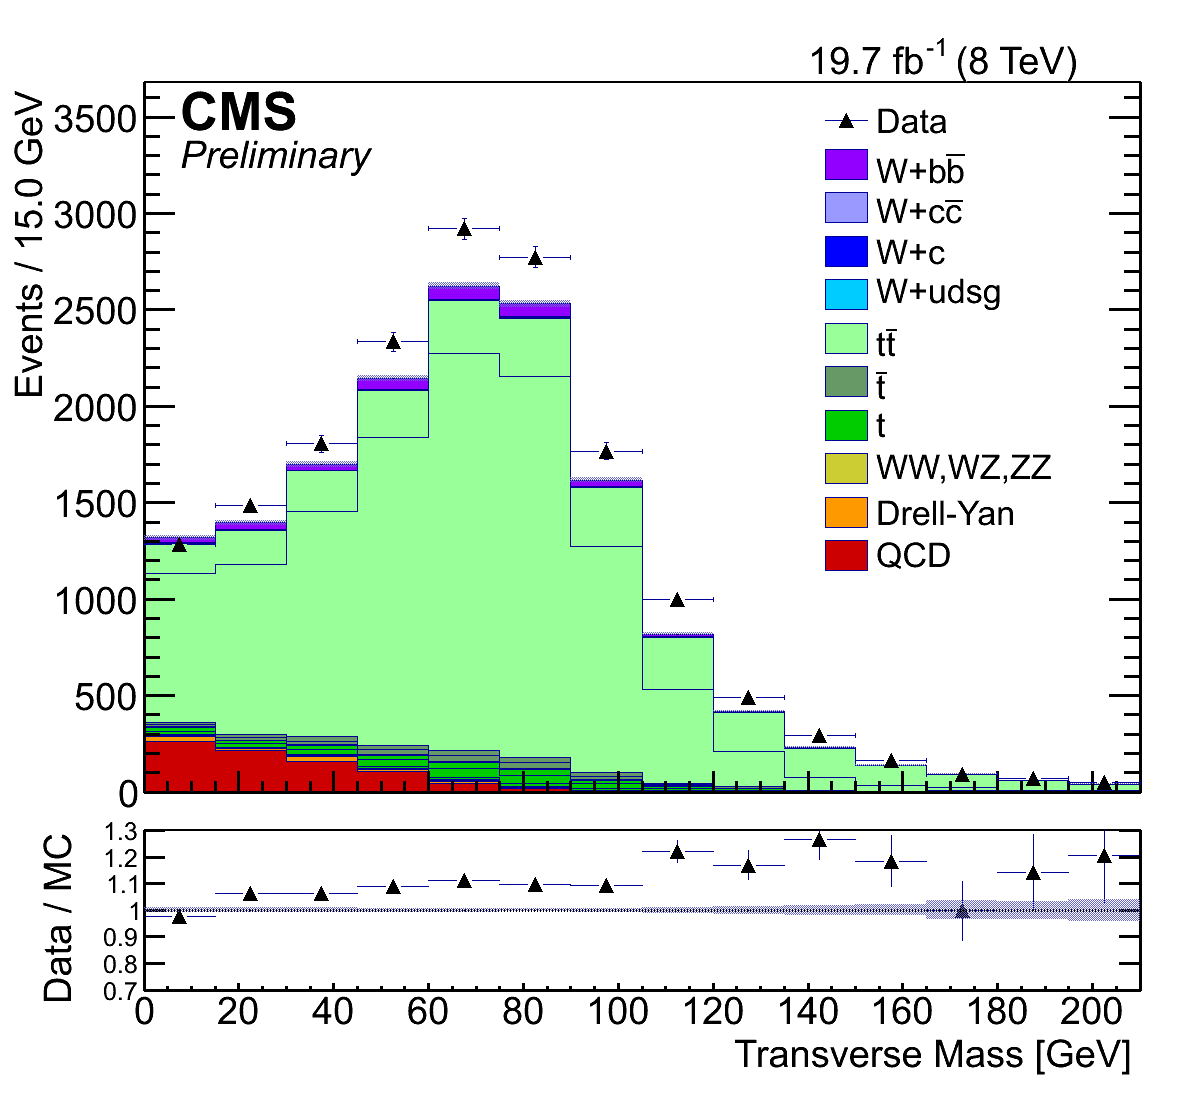
\includegraphics[width=0.4\textwidth]{/Users/rhombus/CMS/Thesis/thesis/pdfs/wbbxc/ttjjj/Histograms_ttjjj_mt_mu.png}
 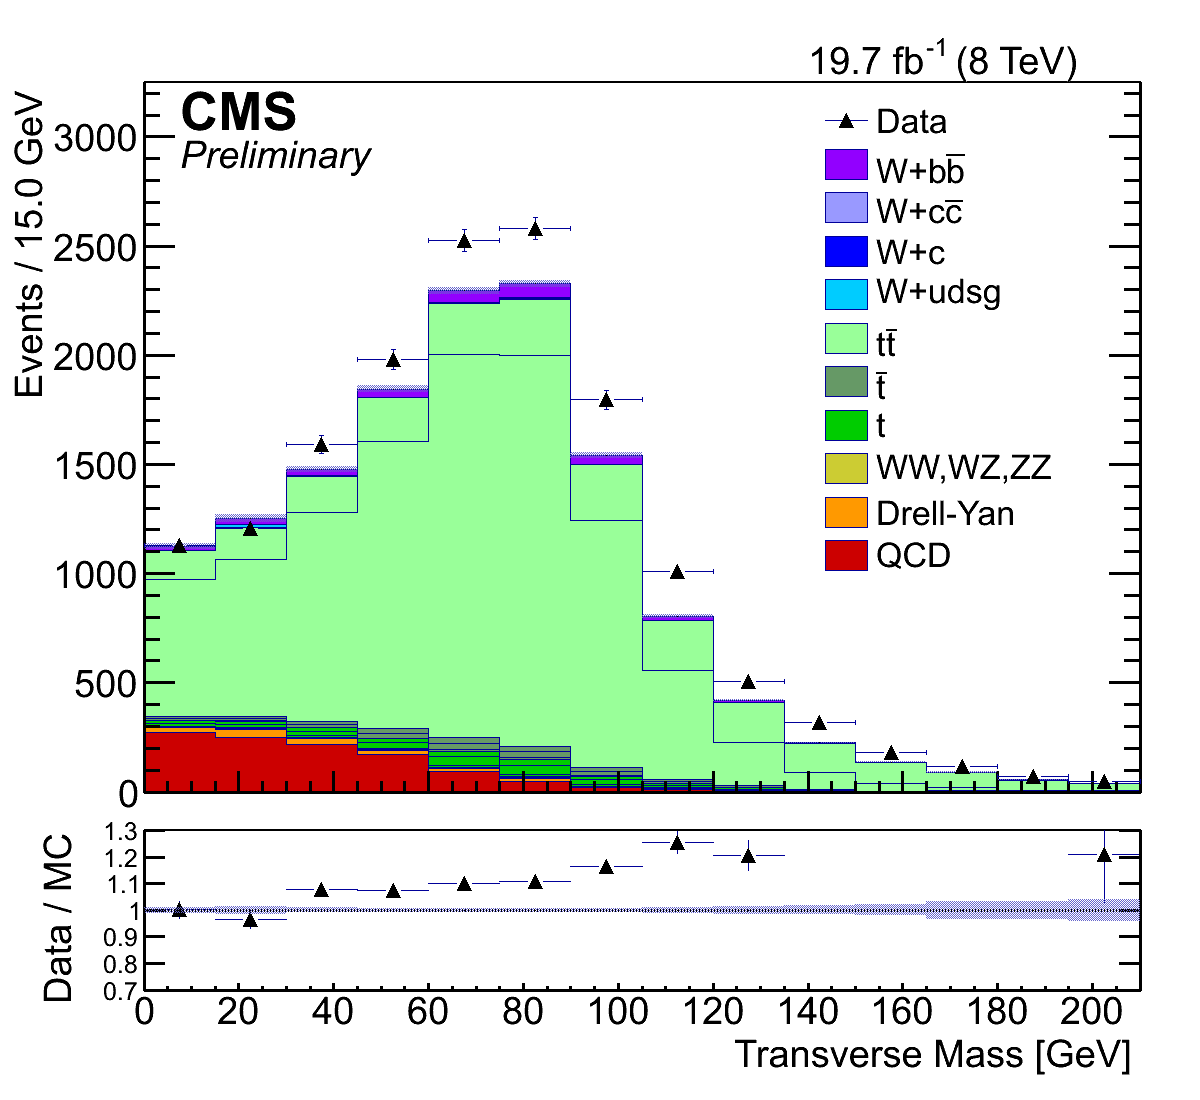
\includegraphics[width=0.4\textwidth]{/Users/rhombus/CMS/Thesis/thesis/pdfs/wbbxc/ttjjj/Histograms_ttjjj_mt_ele.png}
      \label{fig:prefit_ttjjj}
\end{figure}


The selections for the multilepton region differ from those for
 the $\wbb$ region in that exactly two well-isolated
 opposite-flavor leptons are required. 
Figure \ref{fig:prefit_ttme} shows representative distributions
 in this phase space where $\ttbar$ accounts for over
 95\% of the simulated samples.
%A detailed study of this phase space is presented in 
% Appendix \ref{sec:ttcrosscheck}.

\begin{figure}
      \caption[\ttbar-multilepton control region for the \wbb measurement]
    {Distributions in the $\ttbar$ multilepton control region are shown here in both channels.
       These raw distributions are made before any of the scaling outlined in Section \ref{subsec:wbb_analysisstrategy}.
       Left plots are in the muon decay channel and right
        plots are in the electron decay channel.
      }
      \center
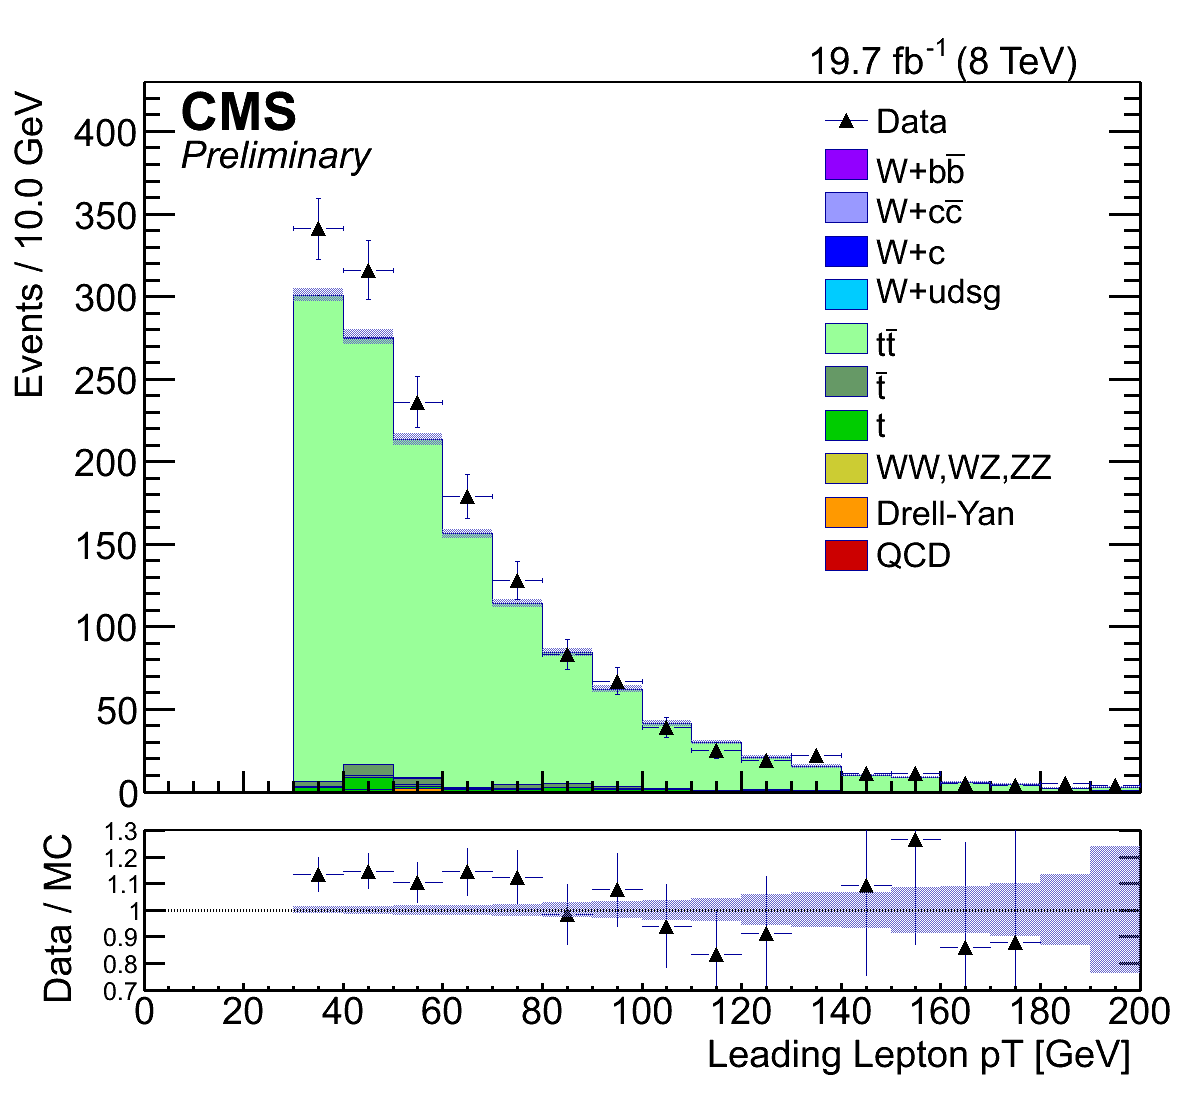
\includegraphics[width=0.4\textwidth]{/Users/rhombus/CMS/Thesis/thesis/pdfs/wbbxc/ttme/Histograms_ttme_goodLep_pt_mu.png}
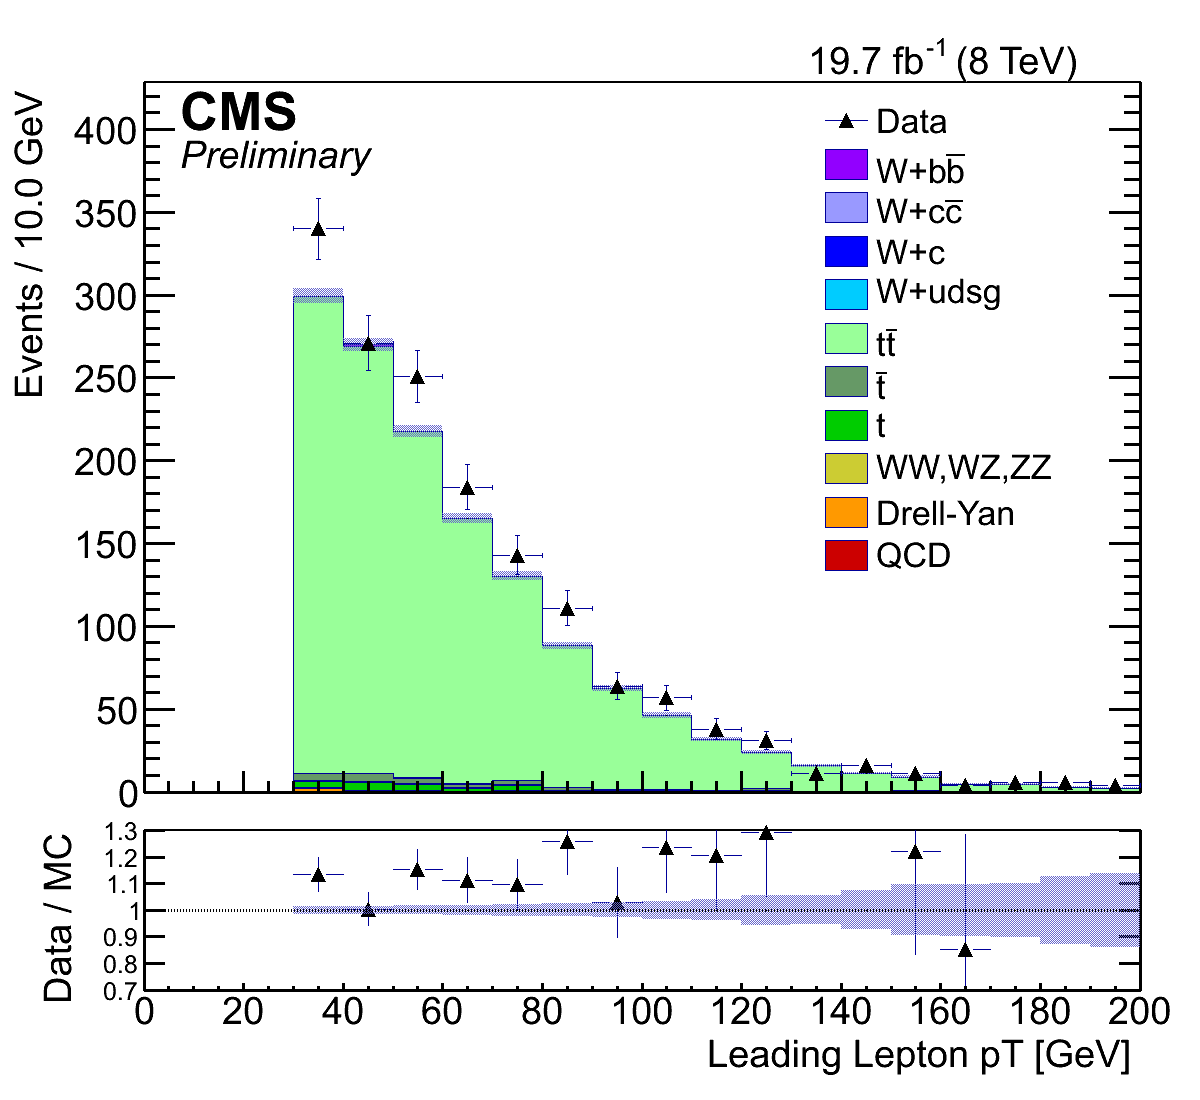
\includegraphics[width=0.4\textwidth]{/Users/rhombus/CMS/Thesis/thesis/pdfs/wbbxc/ttme/Histograms_ttme_goodLep_pt_ele.png}
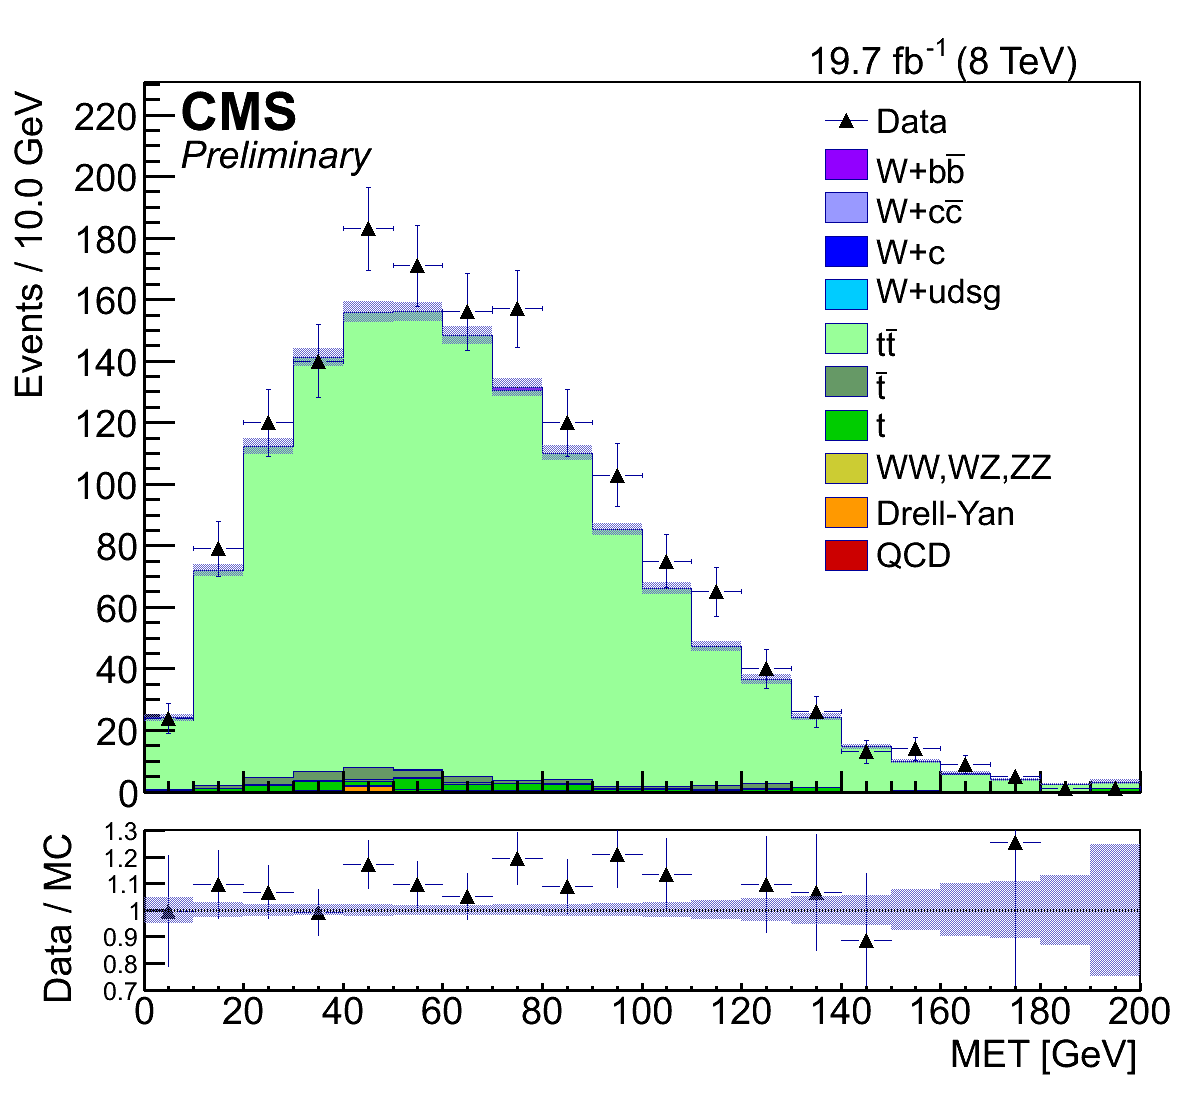
\includegraphics[width=0.4\textwidth]{/Users/rhombus/CMS/Thesis/thesis/pdfs/wbbxc/ttme/Histograms_ttme_met_mu.png}
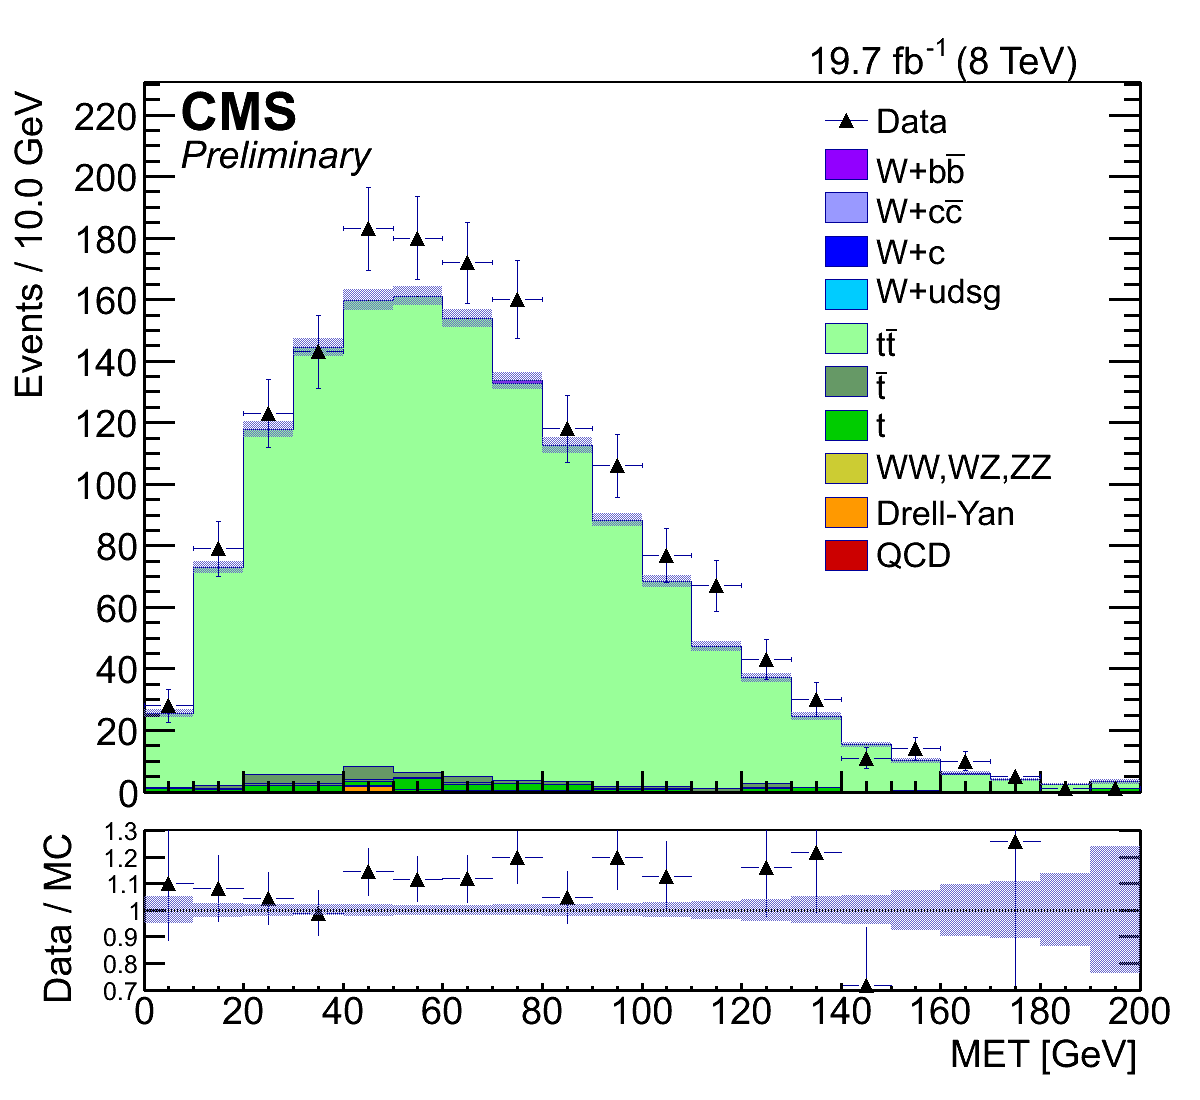
\includegraphics[width=0.4\textwidth]{/Users/rhombus/CMS/Thesis/thesis/pdfs/wbbxc/ttme/Histograms_ttme_met_ele.png}
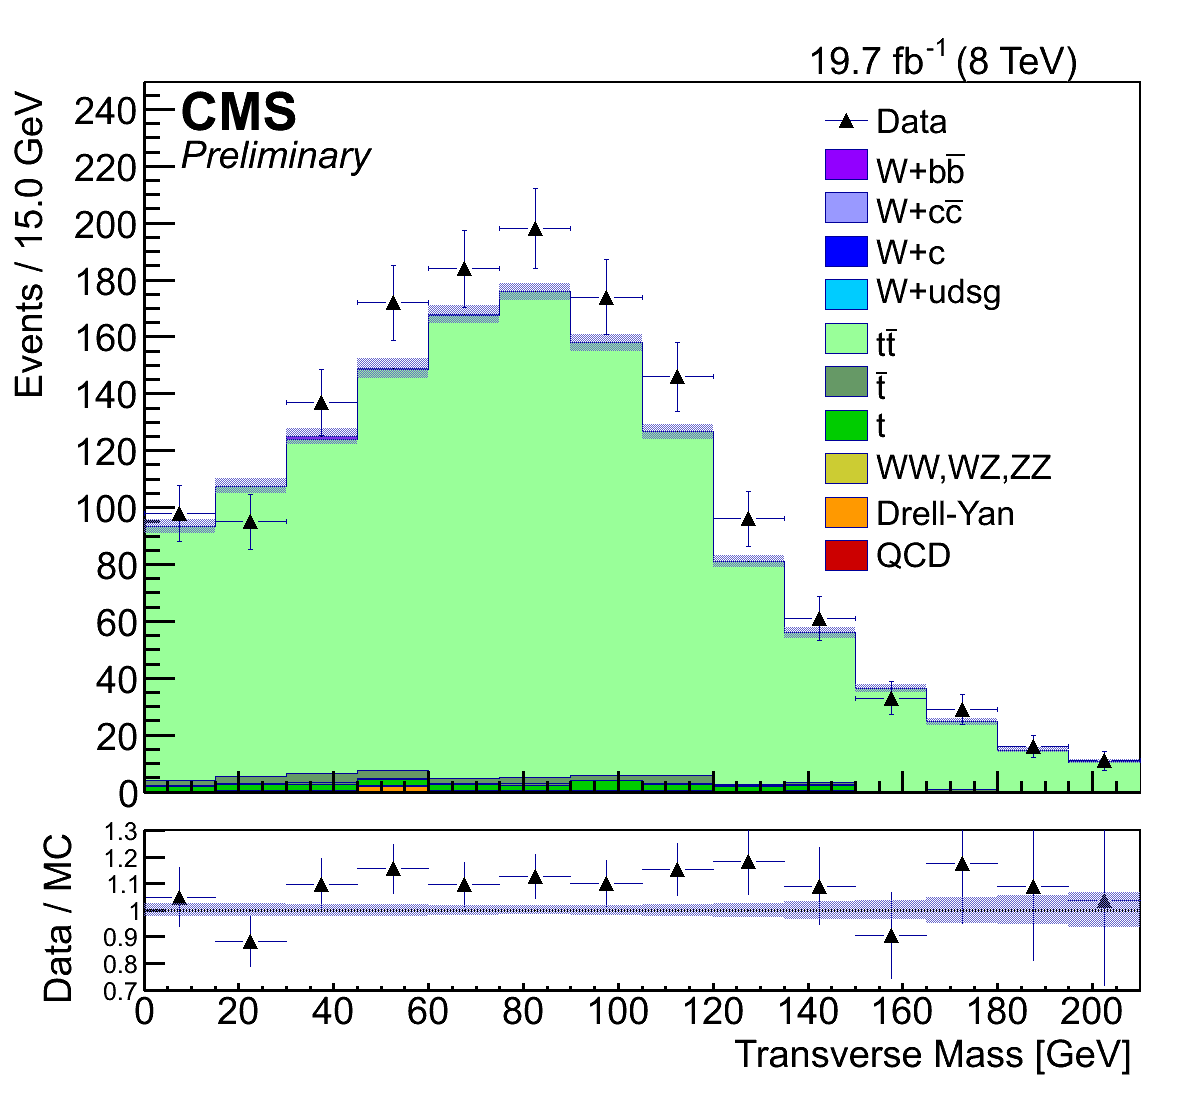
\includegraphics[width=0.4\textwidth]{/Users/rhombus/CMS/Thesis/thesis/pdfs/wbbxc/ttme/Histograms_ttme_mt_mu.png}
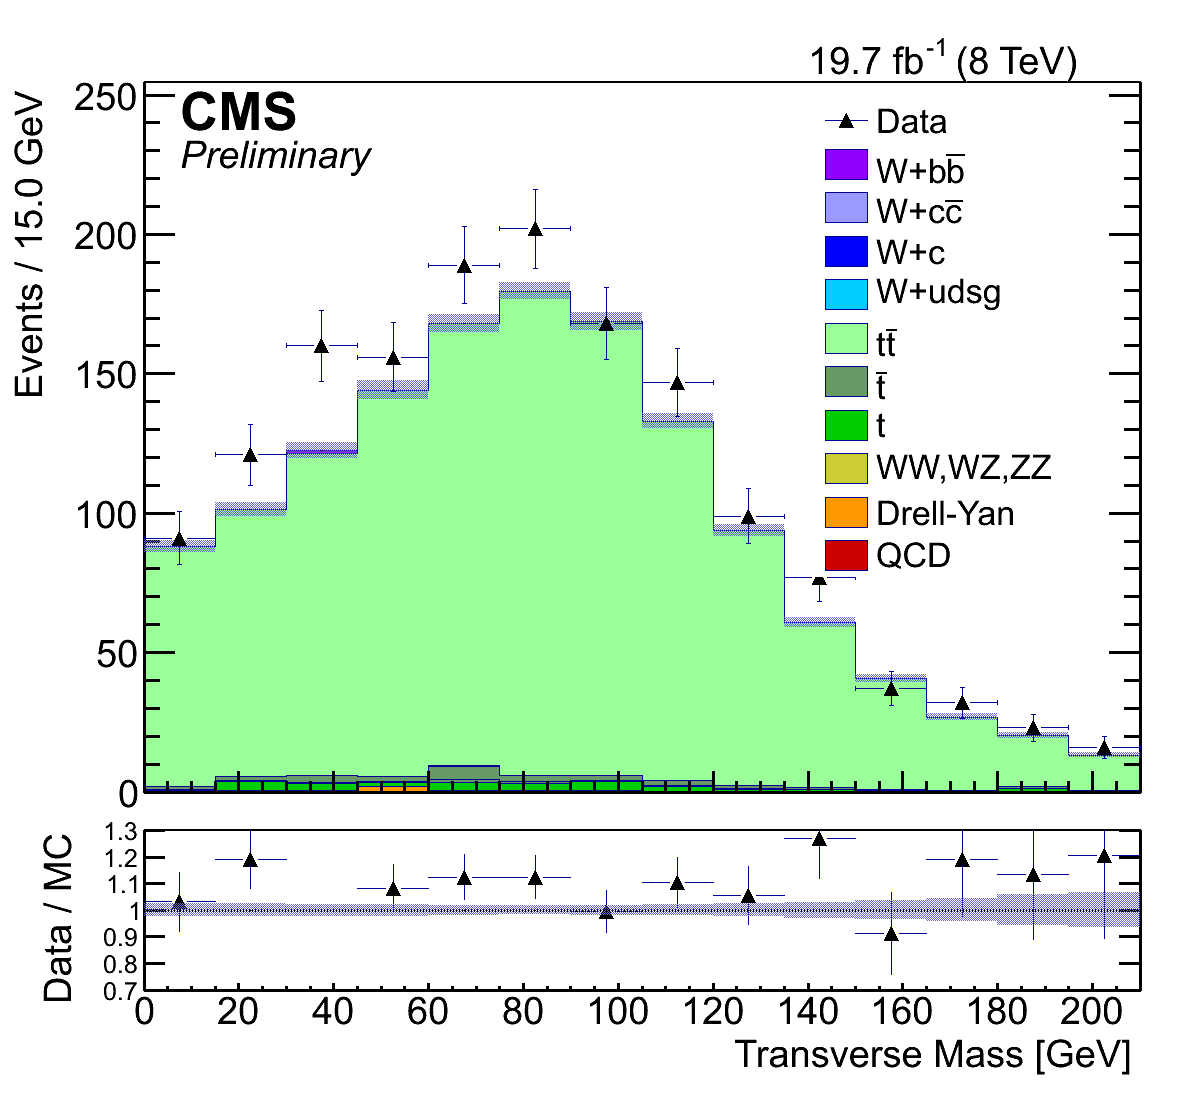
\includegraphics[width=0.4\textwidth]{/Users/rhombus/CMS/Thesis/thesis/pdfs/wbbxc/ttme/Histograms_ttme_mt_ele.png}
      \label{fig:prefit_ttme}
\end{figure}

The single top control region is defined by the signal selection requirements
 without the third and forward jet vetos, and
 with the leading jet required to be central
 ($|\eta|<2.4$) and tightly b-tagged,
 while the subleading jet has no $b$ requirement and must fall within
 $2.4<|\eta|<5.0$.
As illustrated in Figure \ref{fig:prefit_stt}, there are many 
 backgrounds contaminating the purity of this phase space,
 but agreement between data and simulation is on the order of 5-10\%.
\begin{figure}
      \caption[Single-top control region for the \wbb measurement]{The single top control region is defined by one b-tagged central jet and one forward jet.
      Shown above are distributions in the single top control region.
       Left plots are in the muon decay channel and right
        plots are in the electron decay channel.
      }
      \center
 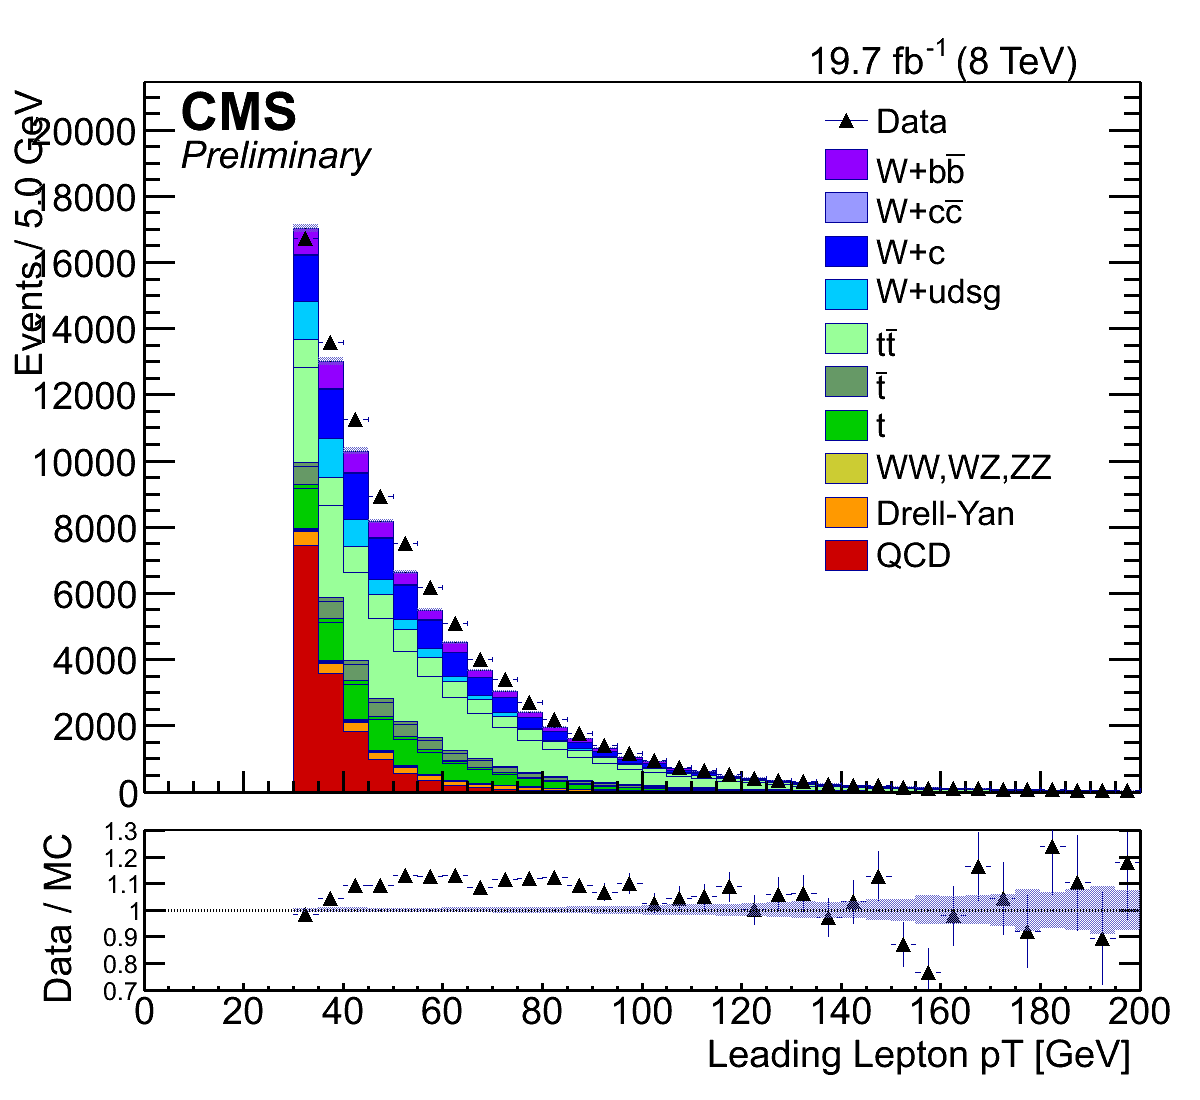
\includegraphics[width=0.4\textwidth]{/Users/rhombus/CMS/Thesis/thesis/pdfs/wbbxc/stt/Histograms_stt_goodLep_pt_mu.png}
 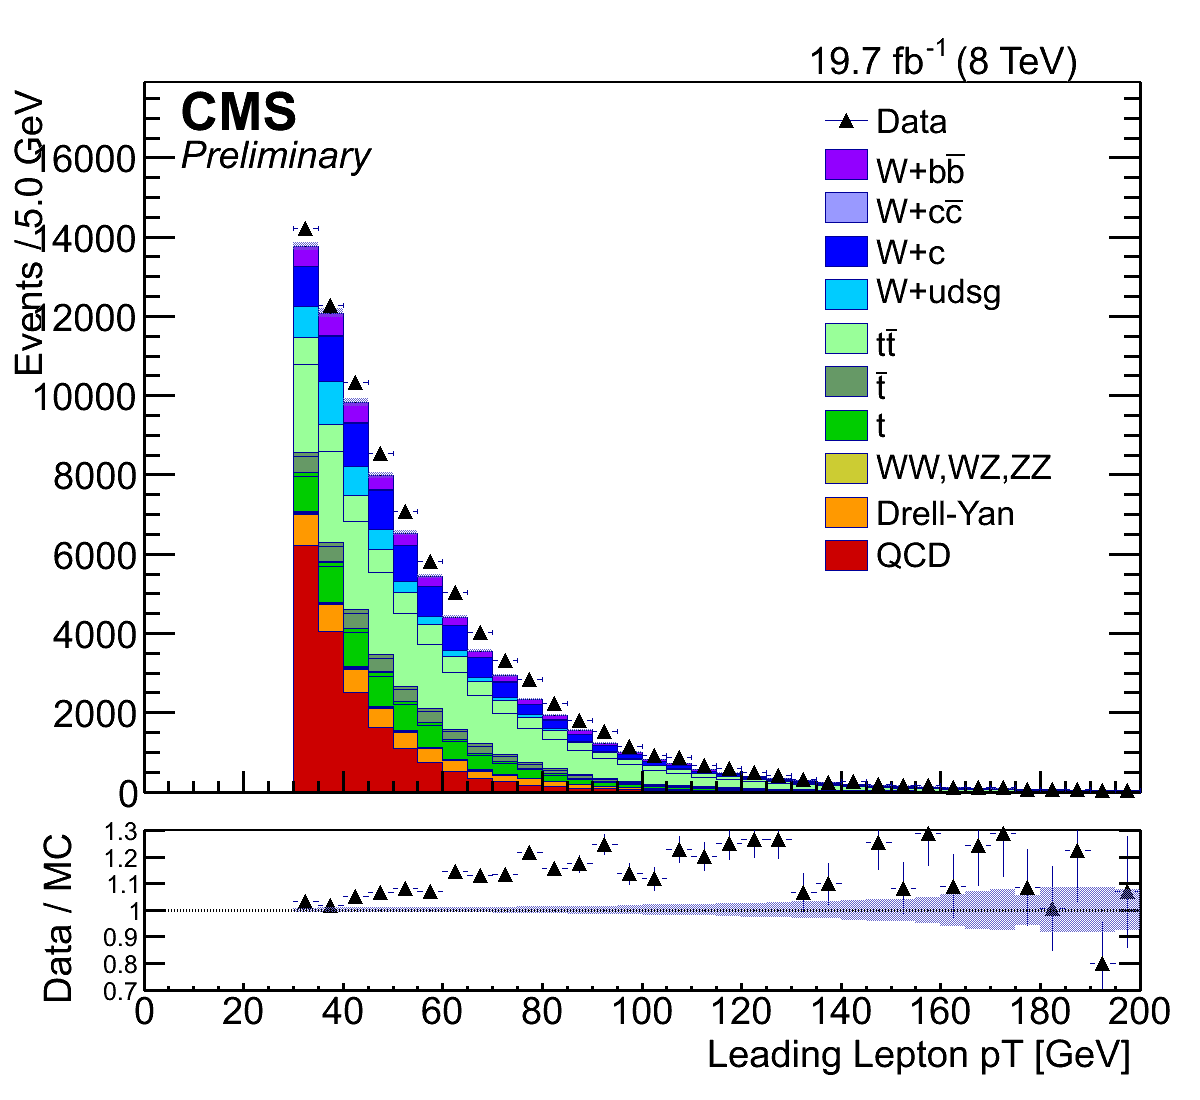
\includegraphics[width=0.4\textwidth]{/Users/rhombus/CMS/Thesis/thesis/pdfs/wbbxc/stt/Histograms_stt_goodLep_pt_ele.png}
 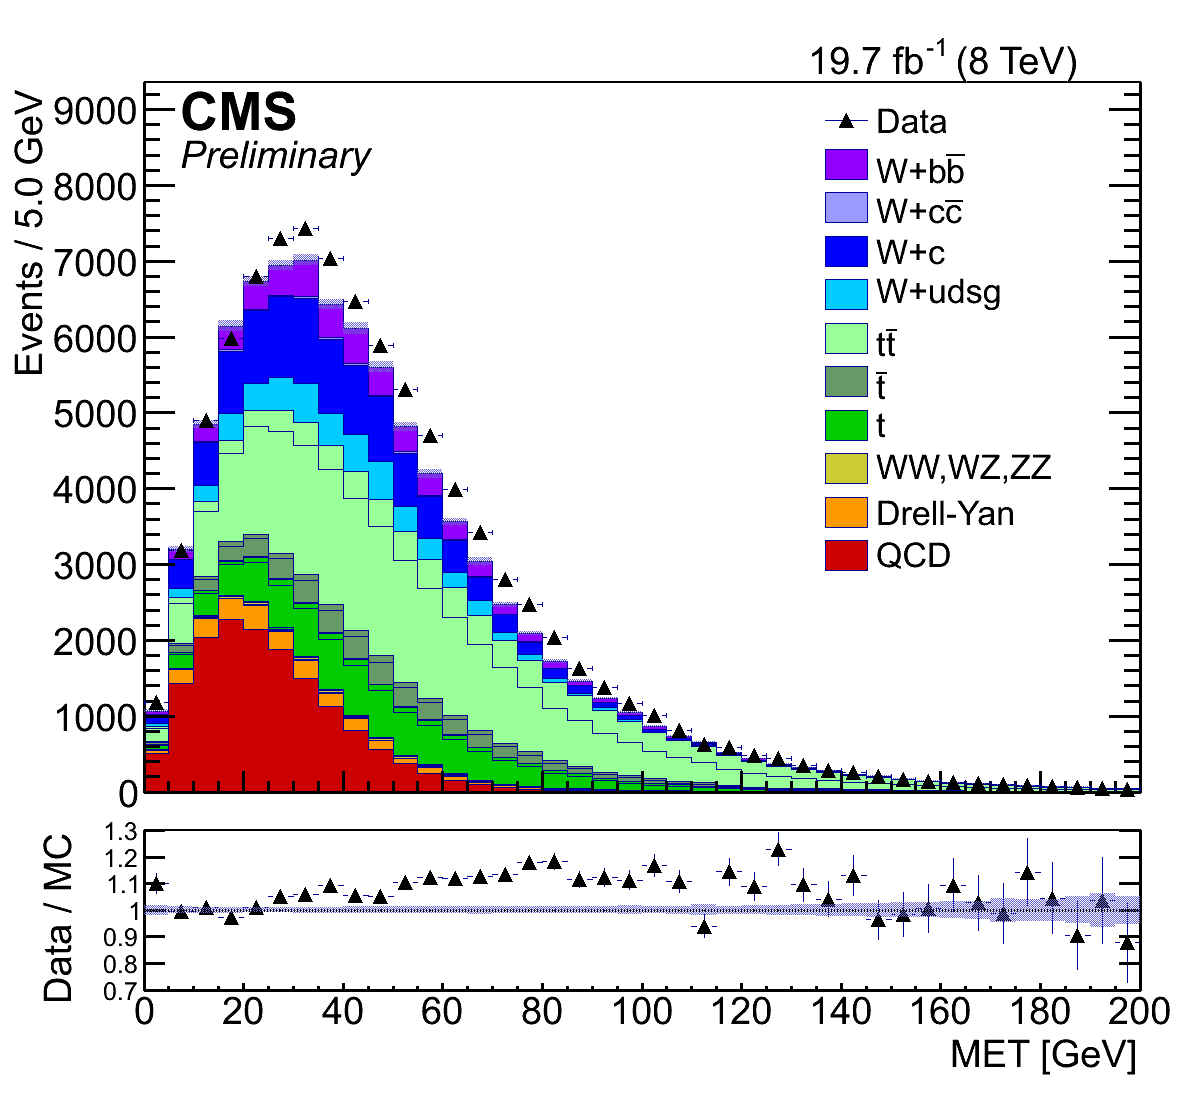
\includegraphics[width=0.4\textwidth]{/Users/rhombus/CMS/Thesis/thesis/pdfs/wbbxc/stt/Histograms_stt_met_mu.png}
 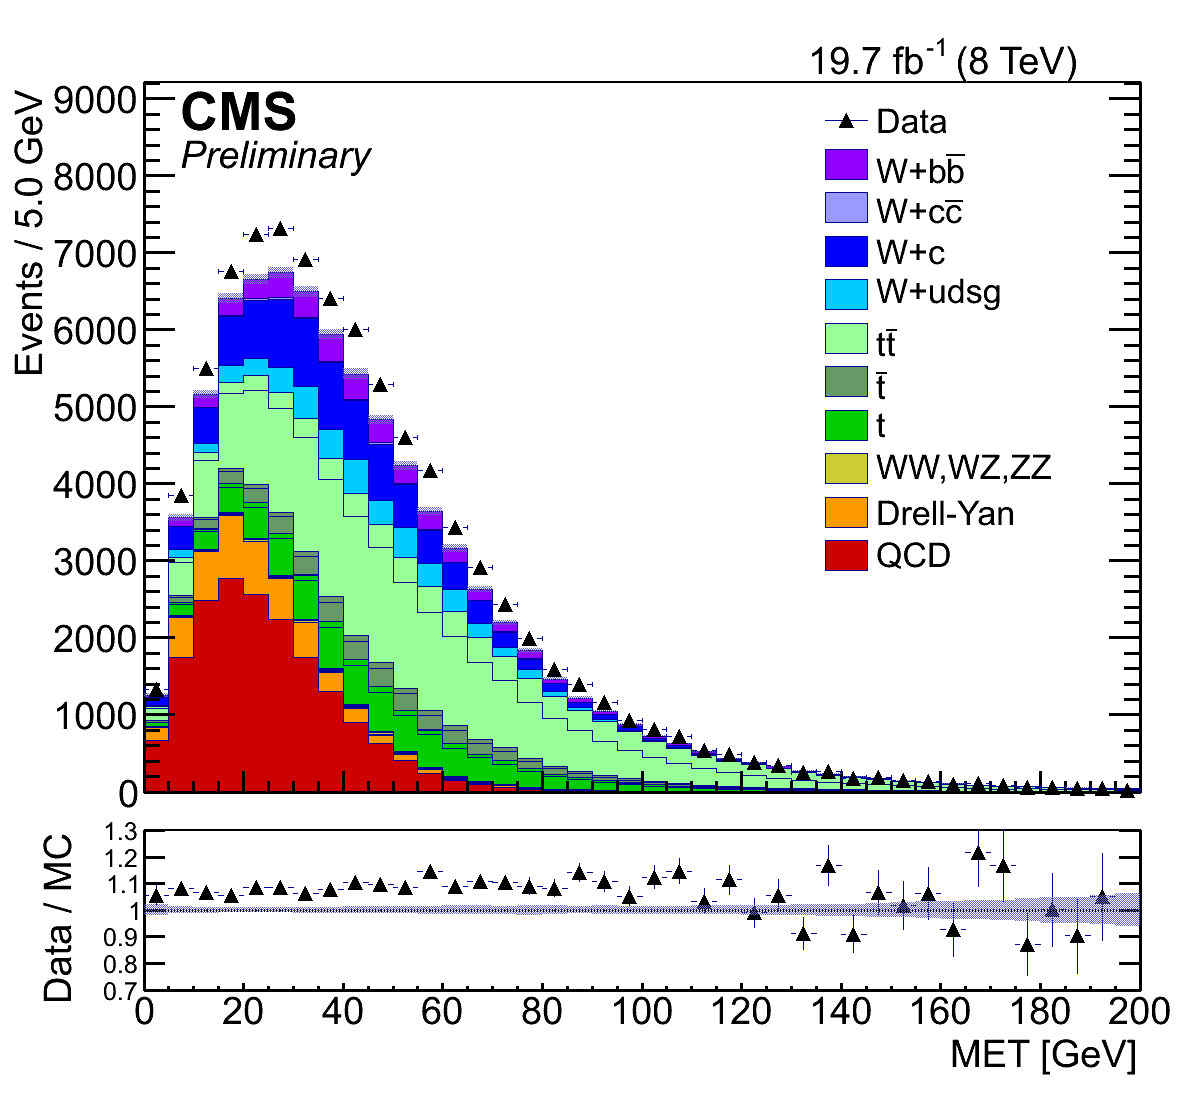
\includegraphics[width=0.4\textwidth]{/Users/rhombus/CMS/Thesis/thesis/pdfs/wbbxc/stt/Histograms_stt_met_ele.png}
 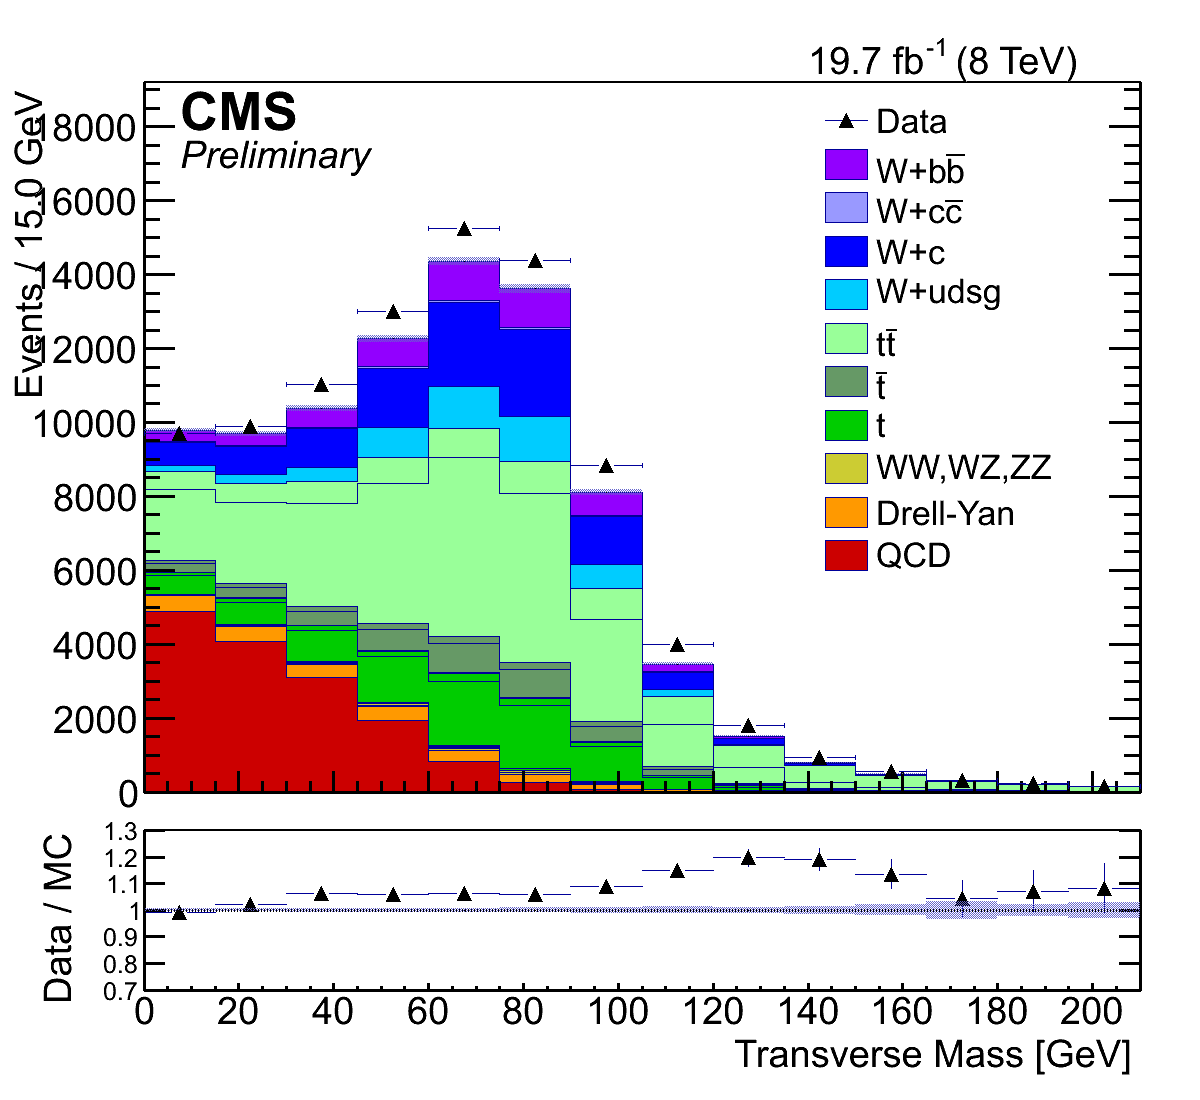
\includegraphics[width=0.4\textwidth]{/Users/rhombus/CMS/Thesis/thesis/pdfs/wbbxc/stt/Histograms_stt_mt_mu.png}
 \includegraphics[width=0.4\textwidth]{/Users/rhombus/CMS/Thesis/thesis/pdfs/wbbxc/stt/Histograms_stt_mt_ele.png}
      \label{fig:prefit_stt}
\end{figure}


\subsection{\zll backgrounds}

The Drell-Yan backround is validated in a control region where the $\wbb$
 selection requirements are applied, but the lepton veto 
 is inverted, requiring two isolated, same-flavor leptons 
 and the $\mt$ requirement is dropped.
This is referred to as the $\zbb$ region and distributions
 of the mass and transverse momentum of the dilepton pair is
 shown in Figure \ref{fig:prefit_dybb}.
Contamination from \ttbar is evident. 
A cleaner Drell-Yan phase space is found by requiring exactly two jets
 but placing no b tag requirement and is referred to as $\zjj$.
Figure \ref{fig:prefit_dyjj} shows the same distributions as
 Figure \ref{fig:prefit_dybb} in this phase space.
%More cross checks on Drell-Yan are shown in Appendix \ref{sec:dycrosscheck}.

\begin{figure}
      \caption[\zbb control region for the \wbb analysis]{ Above are distributions of the mass and
        transverse momentum of the dilepton pair in the
        $\zbb$ phase space.
       Left plots are in the muon decay channel and right
        plots are in the electron decay channel.
      }
      \center
\includegraphics[width=0.4\textwidth]{/Users/rhombus/CMS/Thesis/thesis/pdfs/wbbxc/dy/Histograms_e2CJ_xFJ_tB2_goodL1L2_mass_mu.png}
\includegraphics[width=0.4\textwidth]{/Users/rhombus/CMS/Thesis/thesis/pdfs/wbbxc/dy/Histograms_e2CJ_xFJ_tB2_goodL1L2_mass_ele.png}
\includegraphics[width=0.4\textwidth]{/Users/rhombus/CMS/Thesis/thesis/pdfs/wbbxc/dy/Histograms_e2CJ_xFJ_tB2_goodL1L2_pt_mu.png}
\includegraphics[width=0.4\textwidth]{/Users/rhombus/CMS/Thesis/thesis/pdfs/wbbxc/dy/Histograms_e2CJ_xFJ_tB2_goodL1L2_pt_ele.png}
      \label{fig:prefit_dybb}
\end{figure}

\begin{figure}
      \caption[\zjj control region for the \wbb measurement]{ Above are distributions of the mass and
        transverse momentum of the dilepton pair in the
        $\zjj$ phase space.
       Left plots are in the muon decay channel and right
        plots are in the electron decay channel.
      }
      \center
 \subfloat[]{\includegraphics[width=0.4\textwidth]{/Users/rhombus/CMS/Thesis/thesis/pdfs/wbbxc/dy/Histograms_e2CJ_xFJ_goodL1L2_mass_mu.png}}
 \subfloat[]{\includegraphics[width=0.4\textwidth]{/Users/rhombus/CMS/Thesis/thesis/pdfs/wbbxc/dy/Histograms_e2CJ_xFJ_goodL1L2_mass_ele.png}}
  \\
 \subfloat[]{\includegraphics[width=0.4\textwidth]{/Users/rhombus/CMS/Thesis/thesis/pdfs/wbbxc/dy/Histograms_e2CJ_xFJ_goodL1L2_pt_mu.png}}
 \subfloat[]{\includegraphics[width=0.4\textwidth]{/Users/rhombus/CMS/Thesis/thesis/pdfs/wbbxc/dy/Histograms_e2CJ_xFJ_goodL1L2_pt_ele.png}}
  \\
      \label{fig:prefit_dyjj}
\end{figure}


\section{Analysis Strategy}\label{subsec:wbb_analysisstrategy}
The $\wbb$ yield is ultimately measured using a likelihood fit
 to the $\mt$ distribution in the signal region,
 after having rescaled the simulation. 
Since the dominant background in the signal region arises
 from the $\ttbar$ process, the data and simulation
 are compared in two $\ttbar$-dominated control regions.
The simulation is reweighted to describe the control regions
 and then is used to predict the $\mt$ distributions
 in the signal region.

%The dominant background in the signal
% region arises from the $\ttbar$ process.
%Data and simulation are hence first compared in two 
% $\ttbar$-dominated control regions and 
% MC scale factors are extracted and 
% applied to the signal region.
%Then a likelihood fit is performed to the $\mt$ 
% distribution in order to extract the $\wbb$ cross section.
%In the fit, interpolations are performed as a log normal for
% uncertainties affecting only the normalization
% of distributions
% and quadratically for uncertainties
% affecting both the shapes and normalizations.

The signal region requires a muon (electron)
 with $\pt > 30$ GeV, pseudorapidity
 $|\eta| < 2.1$, and satisfying $I < 0.12~(0.10)$.
 %as defined in Eq. \ref{eq:iso}.
Exactly two b-tagged jets with
 $\pt > 25$ GeV and
 $|\eta| < 2.4$ are also required. %selected for.
Events with additional leptons with
 $\pt > 10$ GeV and $|\eta| < 2.4$ or
 a third jet with $\pt > 25$ GeV and $|\eta| < 5.0$
 are rejected.
The $\ttbar$-multijet control region is obtained
 using the same selection criteria as in the signal region,
 but requiring at least three jets in the event
 with $\pt>25$ GeV and $|\eta|<2.4$ instead of
 vetoing events which have more than two.
The $\ttbar$-multilepton control region uses
 similar selection criteria as the signal region,
 but changing the lepton requirement from vetoing
 events which contain a second lepton,
 to requiring two isolated leptons of different flavor,
 both with $\pt>30$ GeV and $|\eta|<2.1$.

The shape of the $\wbb$ signal distribution is obtained by separating
 the $\wjets$ simulated sample into three subsamples labeled as $\wbb$, $\wcc$, and $\wudscg$.
The separation is done at the truth generator level.
If an event contains a b jet, from matrix element or parton shower,
 it falls into the $\wbb$ category.
A b jet at generator level requires
 the presence of a b hadron within a cone of
 radius $R=0.4$ with respect to the jet axis.
The jets are constructed at the generated level using
 all stable particles in the event (excluding neutrinos).
Jets with a distance smaller than $R = 0.5$ with respect to a
 lepton are removed from the event.
%Exactly two b jets with $\pt>25\GeV$ and $|\eta|<2.4$
% are required in the signal region.
If an event contains no b jets but
 an even, non-zero, number of charm jets,
 again from matrix element or
 parton shower, it falls into the $\wcc$ category.
The remaining events fall into the $\wudscg$ category.
% hen level definitions
The energy of the selected leptons at the generated level is corrected
 for the final state radiation (FSR) by summing up
 the four-momenta of
 all the photons generated within a cone of radius $R = 0.1$
 around the lepton.
Generated leptons originating in simulation from the decay of b hadrons or $\tau$ leptons
 are not considered.

%The normalizations of the simulated backgrounds are allowed to vary in the fit
% within the uncertainties of the corresponding cross sections
% as listed in Table \ref{tab:input_unc_wbb}.

%The shape of the QCD distribution for each region and lepton
% flavor is estimated from data using samples of events that
% pass all the corresponding region requirements,
% but requiring the muon (electron) to be anti-isolated,
% $I > 0.20~(0.15)$.
%The obtained shapes are corrected for the presence of all other
% backgrounds, estimated from simulation.
%Their contribution is less than 1\% of the QCD rate.
%
%The QCD normalization is adjusted in order to describe
% the number of data events at $\mt<20$ GeV,
% after subtracting the non-QCD backgrounds
% obtained from simulation.
%In the fiducial regions used in this analysis, minimal correlation
% is observed between $I$ and $\mt$, validating
% the use of an inverted isolation requirement to obtain
% the QCD shape.

Two major parameters in the simulations
 significantly affect the shape and
 normalization of the simulated distributions:
 the b-tagging efficiency and the jet energy scale (JES).
Both control and signal regions show similar
 sensitivity to the b-tagging efficiency,
 and its adjustment affects all the regions
 in a correlated manner.
The JES affects more the $\ttbar$ predictions
 in the signal and multilepton regions where a veto
 on the third jet is applied.
The effect on the leading jets is moderate,
 but because of the multijet nature of the $\ttbar$ production,
 the JES variations lead to significant migration of jets
 into and out of the veto region.
The $\ttbar$-multijet control region,
 since it has no veto on the third jet,
 is less sensitive to JES.
The same is observed to be true for the $\wbb$ LO sample
 in all regions and may be due in part to the fact that
 $\wbb$ has no additional jets to veto.

The fit procedure thus consists of three steps.
First, using the simulated samples detailed above,
 a fit is performed in the $\ttbar$-multijet reigion
 using the $\mt$ variable.
The result of this fit gives an estimation of the
 b-tagging effeciency rescaling factor, which
 is measured separately in the muon and electron
 channels and averaged. % before being applied.
The reweighted samples are then used in the next step
 where a fit to the $\mt$ variable in the
 $\ttbar$-multilepton region is performed and
 the jet energy scale in simulation is adjusted.
As a result of these two steps, the simulation is
 expected to properly describe the $\ttbar$ contribution
 and the final step is to extract the number of
 $\wbb$ events from a fit in the signal region.

\section{Systematic Uncertainties}
The major sources of the systematic uncertainties are listed in Table \ref{tab:input_unc_wbb}.
 The size of the variation is presented for each uncertainty source
 together with its effect
 on the signal.
Some of the uncertainties affect
 only the normalization of the respective contributions,
 e.g. the uncertainty on the
 theoretical cross sections.
In other cases, the uncertainties affect also the
 shape of the corresponding $\mt$ distributions,
 and these are listed in
 the table under ``norm. + shape".
In the fit procedure, interpolations are performed following a log
 normal distribution for uncertainties affecting only normalizations
 and a quadratic distribution for uncertainties affecting both the shapes and normalizations.

The 50\% uncertainty on the QCD background is taken as a conservative estimate from
 the control region, and increasing this uncertainty does not lead to any change
 in the result of the fit.
The common b-tagging and JES rescaling factor uncertainties
 are set to $\pm100\%$ of the factor itself, allowing the fit to
 remeasure them in the signal region.
The scale uncertainties are estimated by
 changing the renormalization and factorization scales
 up and down by a factor of two.
The PDF uncertainties are estimated from the change in
 acceptance found by varying the
 PDF set.

\begin{table}[htb]
\begin{center}
\caption[Systematic uncertainties in $\wbb$]{
Breakdown of the major sources of systematic
 uncertainty in the \wbb phase space.
The last column indicates the contribution of
 the given systematic to the overall uncertainty
 on the measured cross section. %signal strength.
The uncertainty labeled "b tag rescale" is
 the uncertainty associated with the rescaling
 of the b tag efficiency scale factors.
In the "variation" column, the uncertainties which
 are correlated across all simulated samples and
 affect both shape and normalization are indicated
 by $\sigma_{\mathrm{X}}$ to indicate that an input variation of
 one standard deviation is set on the uncertainty X in the fitting procedure.
UES refers to the energy scale of energy deposits
 not clustered into jets and MES and EES
 refer to the muon and electron energy scales.
The uncertainty labeled as "Id/Iso/Trg" is the uncertainty
 associated with the efficiency of the lepton
 identification, isolation, and triggering.
The uncertainty on the luminosity and the uncertainty
 on the acceptance due to PDF and scale choices are
 not included in the fit, and are
 treated separately.
}
\label{tab:input_unc_wbb}

%\resizebox{\columnwidth}{!}{%
{\renewcommand{\arraystretch}{1.2}
\begin{tabular}{c|c|l|l|l}
\multicolumn{2}{c|}{}                                                         & {}            & {}        & effect on the measured \\
{} & {}                                                                       & uncertainty   & variation & cross section \\
\hline
\hline
 \multirow{11}{*}{\rotatebox{90}{normalization}} & \multirow{8}{*}{\rotatebox{90}{uncorrelated}} & \ttbar        & 7.4\%     & 10.5\%  \\
            {}                                   &           {}                                  & Single Top    & 5.4\%     & 3.3\%  \\
            {}                                   &           {}                                  &    \wudscg    & 13.2\%    & $<2\%$  \\
            {}                                   &           {}                                  &       \wcc    & 8.1\%     & $<2\%$ \\
            {}                                   &           {}                                  &    Diboson    & 8.1\%     & $<2\%$  \\
            {}                                   &           {}                                  &  Drell-Yan    & 7.9\%     & $<2\%$ \\
            {}                                   &           {}                                  & $\gamma$+jets & 10.0\%    & $<2\%$ \\
            {}                                   &           {}                                  &        QCD    & 50\%      & 1-4\% \\
\cline{2-5}
\noalign{\smallskip}
\cline{2-5}
            {}                                   &\multirow{9}{*}{\rotatebox{90}{correlated}}    & b tag rescale & 12.9\%              & 13.0\% \\
            {}                                   &           {}                                  & JES rescale   & $1.3\times\sigma_{\mathrm{JES}}$ & $3.6\%$ \\
\cline{1-1} \cline{3-5}
 \multirow{5}{*}{\rotatebox{90}{norm. + shape}}  &           {}                                  & JES           & $\sigma_{\mathrm{JES}}$ & 5.6\%  \\
            {}                                   &           {}                                  & UES           & $\sigma_{\mathrm{UES}}$ & 2.8\% \\
            {}                                   &           {}                                  & MES           & $\sigma_{\mathrm{MES}}$ & 3.6\% \\
            {}                                   &           {}                                  & EES           & $\sigma_{\mathrm{EES}}$ & $<2\%$ \\ %$3.5\% \\ 
            {}                                   &           {}                                  & Id/Iso/Trg    & $\sigma_{\mathrm{Id/Iso/Trg}}$ & $<2\%$ \\
\hline
\hline
            \multicolumn{3}{c|}{luminosity}         & \multicolumn{2}{c}{2.6\%}  \\
            \multicolumn{3}{c|}{theory (scale+PDF)} & \multicolumn{2}{c}{10\%}   \\


\end{tabular}
}
%\end{adjustwidth}
\end{center}
\end{table}

\section{Signal Extraction}

\label{sec:results}

The fit in the $\ttbar$-multijet region
 is used to obtain rescaling factors for
 the muon and electron channels separately
 to better describe the
 b-tagging efficiency in the simulation,
 as presented in Section \ref{subsec:wbb_analysisstrategy}.
The results of the fit are presented in Fig. \ref{fig:step1_ttjjj_fitted}.
The measured rescaling factors, $1.17 \pm 0.12$ (muon channel) and
 $1.13 \pm 0.11$ (electron channel), are averaged to $1.15 \pm 0.14$, where
 the uncertainty allows the following fits to
 vary the rescaling factor between 1.01 and 1.29.
 %and with the bounds given by the fits in the individual channels.
The simulation is rescaled accordingly for the next fit and
 the uncertainty on the rescaling is included in the fit procedure.

\begin{figure}[htbp]
\caption[$\ttbar$-multijet control region after fitting for b-tag scale]
 {
  The transverse mass distributions in the $\ttbar$-multijet phase space after fitting to obtain the b-tag rescale factors.
  The lepton channels are shown separately with the muon sample on the left and the electron sample on the right.
  The highest bin contains overflow events.
 The shaded area represents the total uncertainty on the simulation as output from the fit.
 }
\center
\includegraphics[width=0.49\textwidth]{/Users/rhombus/CMS/Thesis/thesis/pdfs/wbbxc/pape/poststep1_ttjjj_mt_mu}
\includegraphics[width=0.49\textwidth]{/Users/rhombus/CMS/Thesis/thesis/pdfs/wbbxc/pape/poststep1_ttjjj_mt_ele}
\label{fig:step1_ttjjj_fitted}
\end{figure}

A fit to the $\ttbar$-multilepton region adjusts
 the jet energy scale, as described in Section \ref{subsec:wbb_analysisstrategy}.
%The energy scale in the fit varies within its uncertainties, $\sigma_{\mathrm{JES}}$.
As a result, the simulated $\mt$ distributions
 change both the shape and normalization.
The best fit suggests changing the
 JES by approximately 1.3$\sigma_{\mathrm{JES}}$ from its central value.
Figure \ref{fig:step2_ttme_fitted}
 shows the results of the fits in the $\ttbar$-multilepton
 enhanced data set for
 the muon channel (left)
 and the electron channel (right).
The JES is therefore shifted by 1.3$\sigma_{\mathrm{JES}}$ in
 the simulation with the uncertainty
 set to 1.3$\sigma_{\mathrm{JES}}$.
Thus the simulation is tuned to describe the $\ttbar$
 control regions and is
 used to extract the signal yield in the signal region.

\begin{figure}[htbp]
\caption[$\ttbar$-multilepton control region after fitting for JES]{
  The transverse mass distributions in the $\ttbar$-multilepton enhanced data set after
   fitting to find the appropriate jet energy scale.
  The lepton channels are shown separately with the muon sample on the left and the electron sample on the right.
  The highest bin contains overflow events.
 The shaded area represents the total uncertainty on the simulation as output from the fit.
 }
\center
\includegraphics[width=0.49\textwidth]{/Users/rhombus/CMS/Thesis/thesis/pdfs/wbbxc/pape/poststep2_ttme_mt_mu}
\includegraphics[width=0.49\textwidth]{/Users/rhombus/CMS/Thesis/thesis/pdfs/wbbxc/pape/poststep2_ttme_mt_ele}
\label{fig:step2_ttme_fitted}
\end{figure}

The results of the fit in the $\wbb$ signal region
 are presented in Fig. \ref{fig:step3b_wbb_fitted}.
All background contributions are allowed to vary
 in the fit within their uncertainties,
 while the $\wbb$ normalization remains a free parameter of the fit.
The correlation between different sources of uncertainties
 is taken into account.
The composition of the event sample in
 the signal region is summarized in Table \ref{tab:wbb_yields}.
Events coming from the production of a Higgs boson in association
 with a vector boson constitute a negligible fraction of the
 overall event yield.

Distributions for variables other than those being directly fitted are
 also produced by applying the results from the three fits to
 the simulated samples.
In the signal phase space, lepton isolation was found to be essentially uncorrelated
 with the shape of the transverse mass variable for QCD events,
 but this was not the case for the $\Delta R$ distance between the
 two b-tagged jets, $\Delta R(\mathrm{\bbbar})$, or the lepton $\pt$.
The shape of the QCD distribution for these variables was therefore
 taken from an $\mt<30$ GeV sideband (as opposed to the inverted isolation
 sideband used for the $\mt$ variable) and the normalization
 set to the final fitted normalization given in Table \ref{tab:wbb_yields}.
Distributions of $\Delta R(\mathrm{\bbbar})$ and $\pt^\ell$ in the
 combined lepton channel are presented in Fig. \ref{fig:postfit_drbb_ptl}.
Agreement between data and simulation is observed.

% mt postfit combined lepton fit
\begin{figure}[!htb]
\caption[Fitted \mt in the \wbb signal region]{
  Transverse mass distributions in the $\wbb$ signal region after
   fitting simultaneously muon and electron decay channels.
  The lepton channels are shown separately with the muon sample on the left and the electron sample on the right.
  The highest bin contains overflow events.
  The shaded area represents the total uncertainty on the simulation as output from the fit.
 }
\center
\includegraphics[width=0.49\textwidth]{/Users/rhombus/CMS/Thesis/thesis/pdfs/wbbxc/pape/postcfit_wbb_mt_mu}
\includegraphics[width=0.49\textwidth]{/Users/rhombus/CMS/Thesis/thesis/pdfs/wbbxc/pape/postcfit_wbb_mt_ele}
\label{fig:step3b_wbb_fitted}
\end{figure}

% Final Fitted Yields
\begin{table}[!htb]
\begin{center}
\caption[Initial and final yields in the $\wbb$ signal region]{
 Initial and final yields obtained in the $\wbb$ signal region.
 The uncertainties on the signal strength represent the
  total uncertainty of the measurement.
}
\label{tab:wbb_yields}
 \begin{tabular}{r|l|l|l|l}
{}       & \multicolumn{2}{c|}{muon}   & \multicolumn{2}{c}{electron}   \\
{}       & Initial      & Fitted      & Initial       & Fitted       \\
\hline \hline
Data     & \multicolumn{2}{c|}{7432}   & \multicolumn{2}{c}{7357}     \\
\hline
\wbb           & 1322.7 & 1731.0 & 1120.5 & 1495.3  \\
\wcc           &   59.7 &   57.4 &   36.0 &   37.2  \\
\wudscg        &  181.7 &  173.8 &  220.0 &  214.3  \\
\ttbar         & 3048.6 & 3276.8 & 2639.6 & 2891.7  \\
Single Top     &  958.0 &  980.1 &  820.2 &  855.5  \\
Drell-Yan      &  261.2 &  262.3 &  220.4 &  225.1  \\
Diboson        &  175.4 &  178.9 &  138.9 &  144.4  \\
$\gamma+$jets  &    0.0 &    0.0 &   98.3 &  104.7  \\
QCD            & 1109.0 &  816.9 & 1653.8 & 1348.0  \\
\hline
\hline
Signal strength & \multicolumn{2}{c|}{$1.21\pm0.24$} &  \multicolumn{2}{c}{$1.35\pm0.28$} \\
\hline
Combined        & \multicolumn{4}{c}{$1.29\pm0.22$} \\
 \end{tabular}
\end{center}
\end{table}

% dR(jj) and pT(l) postfit 
\begin{figure}[!htb]
\caption[Fitted $\Delta R(b\overline{b})$ and $\pt^\ell$ in the \wbb signal region]{
  Distributions of $\Delta R(\mathrm{b\bar{b}})$ and $\pt^\ell$ after
   applying the results from the fits to the simulation.
  The QCD shape was taken from an $\mt<30$ GeV sideband and the
   electron and muon channels have been combined in these distributions.
  The highest bin contains overflow events and
   the shaded area represents the total uncertainty on the simulation as output from the fit.
 }
\center
\includegraphics[width=0.49\textwidth]{/Users/rhombus/CMS/Thesis/thesis/pdfs/wbbxc/pape/postcfit_wbb_dRJ1J2}
\includegraphics[width=0.49\textwidth]{/Users/rhombus/CMS/Thesis/thesis/pdfs/wbbxc/pape/postcfit_wbb_pTLep}
\label{fig:postfit_drbb_ptl}
\end{figure}

\section{Cross Section and Comparisons}

The cross section for the $\wbb$ process,
 $\sigma(\ppwbb)$,
 is derived from the signal strength measurement as obtained from the fit.
The cross section is written as

$$\sigma(\ppwbb) = 
\frac{N^{\mathrm{Data}}_{\mathrm{signal}}}{A\cdot\epsilon\cdot \mathcal{L}} = 
\frac{N^{\mathrm{Data}}_{\mathrm{signal}}}{(N^{\mathrm{MC}}_{\mathrm{signal}}/N^{\mathrm{MC}}_{\mathrm{generated}})\cdot \mathcal{L}} =
%\frac{N_{\mathrm{signal}}}{N_{\mathrm{rec}}} \cdot \frac{N_{\mathrm{gen}}}{\mathcal{L}} = 
\alpha \sigma_{\mathrm{gen}}$$
 where
 $N^{\mathrm{Data}}_{\mathrm{signal}}$ is the number of observed signal events,
 $N^{\mathrm{MC}}_{\mathrm{signal}}$ is the number of expected signal events from simulation,
 $N^{\mathrm{MC}}_{\mathrm{generated}}$ is the number of generated events in the fiducial region,
 $A$, $\epsilon$ are the acceptance and efficiency correction factors,
 $\alpha$ is the measured signal strength in the given lepton channel, and
 $\sigma_{\mathrm{gen}}$ is the simulated fiducial cross section of the signal sample.

In this analysis, the fiducial cross section was calculated in the following manner:
 Madgraph is used to compute the $\wbb$ cross section with fiducial cuts applied.
Then a k-factor for inclusive W production is applied, obtained from the ratio
of the inclusive W cross sections calculated with \FEWZ (at NNLO using the five-flavour
\CTEQ6M PDF set) and with Madgraph.
%In this analysis, the cross section used was calculated with \textsc{fewz} at NNLO
% using the five-flavor \CTEQ6M PDF set on the inclusive $\wjets$ sample.
The product $A\cdot\epsilon$ is 11~(13)\% in the
 muon (electron) channels and results from the
 combined effect of the efficiency from
 lepton identification requirements (80\%), and b tag efficiency (40\% per jet).
The uncertainty on this product is 10\% as listed in the bottom row of
 Table \ref{tab:input_unc_wbb}, which was calculated by varying the PDF
 set using the LHAPDF/PDF4LHC \cite{LHAPDF,Botje:2011sn,Alekhin:2011sk,Ball:2012cx}
 prescription considering
 PDF sets from \CTEQ, \MSTW, \NNPDF, and \HERA
 as well as varying the
 choice of scales
 $\mu_{\mathrm{F}}$, $\mu_{\mathrm{R}}$ simultaneously
 up and down by a factor of two.

The $\wbb$ cross section is measured within a fiducial volume, which is defined by
requiring leptons with $\pt > 30\GeV$ and $\abs{\eta}<2.1$ and exactly two b-tagged jets of
 $\pt > 25\GeV$ and $\abs{\eta}<2.4$.
The measured cross sections are presented in Table \ref{tab:crosssections}.
The combination of the muon and electron measurements is done using a simultaneous fit to both channels,
 taking into account correlations between different sources of uncertainties.

\begin{table}[htbp]
\begin{center}
\caption[Measured cross sections for \ppwbblnbb]{
 Measured cross sections in the muon, electron, and combined lepton channels.}
\label{tab:crosssections}
 \begin{tabular}{l|c}
 Channel        & $\sigma(\ppwbb)$, pb \\

\hline
     Muon & $  0.62 \pm 0.04 \mathrm{(stat)} \pm 0.14 \mathrm{(syst)} \pm 0.06 \mathrm{(theo)} \pm 0.02 \mathrm{(lumi)} $ \\
 Electron & $  0.69 \pm 0.05 \mathrm{(stat)} \pm 0.19 \mathrm{(syst)} \pm 0.07 \mathrm{(theo)} \pm 0.02 \mathrm{(lumi)} $ \\
 Combined & $  0.66 \pm 0.03 \mathrm{(stat)} \pm 0.14 \mathrm{(syst)} \pm 0.07 \mathrm{(theo)} \pm 0.02 \mathrm{(lumi)} $ \\
 \end{tabular}
\end{center}
\end{table}


% 
The measured cross sections are compared to theoretical predictions from
 \MCFM \cite{Campbell:2010ff, Badger:2010mg}
 with the {\MSTW2008} PDF set, as well as from
 %with the {\MSTW2008} NNLO PDF set, as well as from
 \MADGRAPH5
 interfaced with \PYTHIAs in the four- and five-flavour schemes and
 \MADGRAPH5 with \PYTHIAe \cite{ref:Pythia8} in the four-flavour scheme.
In the five-flavour scheme, the PDF set {\CTEQ6L} was
 used and \PYTHIAs was run using {TuneZ2*}.
The two four-flavour samples were produced using
 a NNLO PDF set interfaced with %NNLO23\_lo\_as\_0130\_qed
 \PYTHIA (version 6 in one sample, version 8 in the other)
 in the {CUETP8M1} tune.

% motivation
Comparisons between the results of calculations performed
 under different assumptions provide important feedback
 on the functioning and validity of the techniques employed.
Differences in predictions arising from the modelling of
 b quarks as massive or massless are possible, as are
 variations in predictions arising from the use of different
 showering packages (\PYTHIAs vs.\ \PYTHIAe) or matrix element
 generators (\MADGRAPH vs.\ \MCFM).
In the phase space explored here, these predictions are all
 very close in their central value and agree with each other
 well within their respective uncertainties.

% b -> B
The \MCFM cross section calculation is
 performed at the level of parton jets and thus
 requires a hadronization correction.
The multiplicative hadronization correction factor $0.81\pm0.07$
 is calculated using the \MADGRAPH + \PYTHIAs sample
 and agrees well with a
 similar factor calculated in the $7\TeV$ Z+b analysis
 calculated as $0.84\pm0.03$  \cite{Chatrchyan:2014dha}.
The correction factor is obtained for
 jets computed excluding neutrinos from the particle list, as
 such jets are closer in kinematics
 to particle jets at the detector level.
The uncertainty reflects both the statistics of the
 \MADGRAPH + \PYTHIAs sample as well as a comparison with the
 \MADGRAPH + \PYTHIAe sample.

% DPS
The \MCFM and four-flavour \MADGRAPH predictions do not account for
 \wbb production where the \bbbar system comes from multiple parton scattering.
CMS simulations of \MADGRAPH + \PYTHIA events that include
 double parton interaction (DPS) reproduce the $\wjets$ data \cite{Chatrchyan:2013xxa},
 therefore a \MADGRAPH + \PYTHIAe sample of a $\w$ boson produced in association with a
 \bbbar pair coming from DPS
 was generated to study the effect on the fiducial cross section.
Using this dedicated sample, an additive correction $\sigma_{\mathrm{DPS}}$
 is estimated to be $0.06\pm0.06$ pb, where the uncertainty
 is conservatively assigned to be 100$\%$ of the value.

% PDF/scale uncertainty
The uncertainty in the theoretical cross sections arising
 from the choice of PDF is also accounted for,
 using the LHAPDF/PDF4LHC \cite{LHAPDF,Botje:2011sn,Alekhin:2011sk,Ball:2012cx}
 prescription in which
 PDF sets from \CTEQ, \MSTW, \NNPDF, and \HERA are considered.
Uncertainties in the theoretical cross section due to the
 choice of scale are also estimated by varying the scales
 $\mu_{\mathrm{F}}$, $\mu_{\mathrm{R}}$ simultaneously
 up and down by a factor of two.

The resulting cross section predictions in the fiducial
 phase space at the hadron level and including the estimated
 hadronization and DPS corrections when needed
 are compared in Fig. \ref{fig:xc_comparison}
 with the measured value.
Within one standard deviation the predictions agree with the measured cross section.
The results also agree within one standard deviation with previously published $\wbb$
 measurements at 7 \TeV, where
 data are found to be well described by the same predictions.

\begin{figure}[htbp]
\caption[Cross section comparison for \wbb and generators]{
 Comparison between the measured \wbb cross section and
  various QCD predictions.
 The blue error bars on the predictions represent the uncertainty in
  the given sample associated with PDF choice and
  the black bars represent the total uncertainty.
 In the case of the \MADGRAPH + \PYTHIAs (5F) sample,
  the effects of DPS are already included in the generated
  sample so the extra DPS factor was not needed and the blue
  and black error bars overlap perfectly.
 }
\center
\includegraphics[width=0.7\textwidth]{/Users/rhombus/CMS/Thesis/thesis/pdfs/wbbxc/pape/MCXC_Comparison}
\label{fig:xc_comparison}
\end{figure}



\chapter{Monophoton Analysis}\label{sec:lgxc}

 The second analysis presented in this thesis
  is of the monophoton final state discribed 
  in Section~\ref{sec:znngproduction}.
The data are analyzed in the context of the 
 SM process \ppzgnng  in which the \met is interpreted as coming from the
 invisible decay of the \z boson, \znn.
The data are also analyzed
 as a dark matter search under the interpretation 
 that the \met arises from the 
 annihilation of incoming particles into DM 
 and the $\gamma$ is initial state radiation 
 recoiling against thie process. 
Under this interpretation, limits are set on the
 cross section of DM as a function of the 
 mediator mass for vector and axiel-vector models. 
This analysis is performed using protons colliding at
 \s 13 \TeV provided by the LHC and detected by
 the CMS detector.

\section{Event Selection}\label{subsec:lgevent_selection}

The sample of data analyzed was collected using 
 a trigger that requires at least one photon
 HLT SC candidate with $\ptg > 165 \GeV$.
Because photons interact electromagnetically, they 
 are expected to deposit all of their energy in the
 ECAL, while jets typically have a neutral component and 
 deposit some energy in the HCAL as well. 
To increase photon efficiency, the trigger therefore also
 requires at least 90\% of the energy deposited in 
 the calorimeters to be deposited in the ECAL.
This trigger is 98\% efficient at selecting photons
 which pass the other analysis selections.
Events passing the trigger are further required to
 have at least one PF photon with $\ptg > 175\GeV$
 in the barrel fiducial region ($\abs{\eta} < 1.44$).

To distinguish photons from electrons, which leave a similar
 signature of energy deposits in the ECAL and HCAL,
 candidate photons are required
 to not have any associated track seeds in the pixel detector. 
To distinguish photons from jets, selections based on calorimetric
 information and isolation are applied. 
The fraction of energy deposited in the ECAL compared 
 to the total deposit in the calorimeters
 is tightened relative to the trigger to be 95\%
 and the shower shape variable describing the spread
 of the energy deposits in the $\eta$ direction,
  $\sieie$, %described in Section \ref{sec:sieie},
 is required to be $\sieie < 0.0102$. 
Additionally, the photon is required to pass
 the isolation requirements described in Section \ref{sec:photonreco}.

  %Ref.~\cite{Khachatryan:2015iwa},
%encodes the width of the electromagnetic shower in the $\eta$
%direction, which is generally larger in showers from hadronic
%activity. 

Because photon objects are not reconstructed from tracks,
 there is an ambiguity in identifying the collision
 vertex that the photon originates from in the presence 
 of pileup collisions.
Association of a vertex to the photon candidate impacts the photon in two ways. 
First, the photon momentum direction is defined by the
 straight line which connects
 the ECAL cluster position and the identified vertex. 
Additionally, the isolation sum 
 uses only the PF charged hadrons
 having tracks
 associated to the vertex. 
While the first effect is minor and is
 not relevant for this analysis, the second will cause photon
 candidates that are actually not isolated to appear
 isolated, if the 
 vertex is misassigned.  
In practice, photon momentum is always
 computed with respect to the PV,
 but for the charged hadron isolation sum,
 all vertices are considered, and the 
 maximum value of the isolation sum is used as a conservative estimate
 of the true isolation sum.

To reduce the contribution of backgrounds arising from 
 occurances in the CMS detector which did not originate from
 collisions, the energy pulse which seeded the photon cluster
 is required to be within $\pm 3\ns$ of the time expected
 for particles from a collision, and the cluster must not
 be so narrow that it is consistent with a cluster formed by a single crystal.  
To reduce contamination from beam halo, the ECAL
 crystals not  associated with the photon candidate are 
 examined for evidence of the passage of a minimum-ionizing
 particle (MIP) roughly parallel to the beam axis (beam halo tag).
If at least  4.9 \GeV of energy is found deposited along
 this trajectory, the event is rejected.
This value was determined by through optimizing the
 signal to background photon efficiencies, with
 a $95\%$ identification for prompt photons and
 a $20\%$ misidentificatin rate for deposits originating
 in beam halo events.

%To further
%suppress the beam halo background, possible paths of halo muons that
%run through each photon candidate are considered, and the total energy
%deposit in the ECAL along the path that is the most compatible with
%the halo hypothesis is required to be below a threshold, defined to
%achive 95\% efficiency over prompt photons.

%The missing transverse momentum (\ptvecmiss) is defined by the
%magnitude of the vector sum of the transverse momenta of all PF
%candidates in the event. The magnitude of \ptvecmiss is \met. Jets are
%%also formed from PF candidates, and are clustered using the anti-\kt
%algorithm~\cite{Cacciari:2008gp} with a distance parameter of 0.4. Jet
%energies are calibrated to account for pileup effects and detector
%response.

The candidate events are required to have \met $> 170$~\GeV.
%after
%adjusting \ptvecmiss for the difference between simple momentum sums
%of PF candidates and calibrated jet momenta. 
The azimuthal opening
angle between the candidate photon and $\vmet$ is required to be
greater than 2 radians to ensure that the main source of \met is not photon
energy mismeasurement.  

Because jet energy mismeasurement can also
 give rise to \met, events are rejected if the minimum azimuthal opening
 angle between $\vmet$ and up to four leading jets (\minDphiMETj) is
 less than 0.5 radians.
As was the case in the $\wbb$ analysis,
 jets are reconstructed using the PF algorithm, but
 in this analysis the jet clustering cone size is $\Delta R < 0.4$ radians.

Finally, events are also vetoed if they contain 
 a charged lepton (an electron or a muon) with $\pt >
10$ \GeV that is separated from the photon by $\Delta R > 0.5$ radians.

The effects of the various cuts with regard to the 
 total number of events passing selections on the data 
 is illustrated in Table \ref{tab:lgcutflow}.
After applying all of the selection criteria,
 77 candidate events are found in data.

\begin{table}
\caption[Monophoton Cutflow]
{
Listed below are the raw number of events in data 
 passing the selection listed in the first column
 as well as all selections in higher rows.
}
\begin{center}
\begin{tabular}{r|l}
Selection  & Events passing selection \\ 
\hline\hline
 PF photon, $\ptg > 175$ \GeV, $\abs{\eta^\gamma}<1.44$  &   X \\
 $\abs{t^{\mathrm{seed}}}<3$ ns                          &   X \\
 $MIP < 4.9$ \GeV                                        &   X \\
 $\met > 170$ \GeV                                       &   X \\
 $\DphiMETg > 2$ radians                                 &   X \\
 $\DphiMETj > 0.5$ radians                               &   X \\
 Veto charged lepton                                     &   X
\end{tabular}
\end{center}
\label{tab:lgcutflow}
\end{table}

\section{Estimation of Background Contributions}

The dominant SM processes contributing to this 
 phase space of the candidate events 
 are the associated productions of a \z
 or \w boson with a high-energy photon. 
If the \z boson decays into a  neutrino-antineutrino pair, 
 the final state exhibits a high-\et photon and large
 missing transverse energy. 
Similarly, if the \w boson decays into a lepton-neutrino
 pair and  the lepton is outside of the detector acceptance
 or fails reconstruction, the event appears to be \gmet.
 Together, these two processes account for approximately
  75\% of the events as
 estimated using Monte Carlo (MC) simulations. 
Hard-scattering events are generated with \MGfiveAMC\
  version 2.2~\cite{Alwall:2014hca} at leading order (LO) in QCD,
 with  \NNPDFthree LO ($\as = 0.130$) as the parton distribution function.
Parton shower and hadronization is performed by \PYTHIA{}8.2~\cite{Sjostrand:2014zea}.
Generated particles are processed through the full \GEANT-based simulation of the CMS 
 detector \cite{GEANT, GEANTdev} and event reconstruction used for data. 
Minimum-bias simulations are overlaid to model pileup interactions.

 \subsection{Reweighting}\label{subsubsec:lg_reweighting}
To account for differences arising from imperfect modeling of the data in
 the simulation, a total correction factor $\rho = 0.99 \pm 0.06$ is applied to all 
 MC-based  estimates. 
This is the product of individual correction factors which 
 are each taken as the
 ratio of the efficiency measured in data and in simulation.
The efficiency for photon identification is measured
 and provided centrally using \zee events as 
 $0.99\pm0.016$ for photon identification measured using \zee events.
The photon seed trigger efficiency is also measured using \zee events,
 and is found to be $1.00\pm0.0246$ using jet triggers as a reference.
The efficiencies for 
 worst isolation, beam halo tag and lepton veto 
 were measured using events in data which were triggered as having at least
 one muon and on MC using a combination of Drell-Yan, \ttbar and $VV$ 
 samples requiring \zgmmg events to be identified by
 the dimuon pair with mass in the range $61<m_{\mu\mu}<121$ \GeV.
The measured relative efficiencies are $1.00\pm0.05$.

Generated samples are weighted on an event by event basis with a product of two factors. 
The first factor matches the distribution of the generator-level photon
 \pt to that calculated at next-to-next-to-leading order (NNLO) in QCD using the 
 \DYRes~\cite{Catani:2015vma} calculator and
 the second factor, taken from
 Refs.~\cite{Denner:2014bna,Denner:2015fca}, further corrects this distribution
 to account for electroweak next-to-leading order (NLO) effects. 

%\begin{figure}[htb]
%\caption[Distributions of \pt and \met in the \pploneg analysis]
% {The photon \pt and \met\ distribution for the candidate sample,
%  compared with estimated contributions from SM backgrounds, 
%  here QCD$\gamma$ refers to $\gamma$+jet background and the
%  background uncertainity includes statistical and systematic error. }
%\centering
%\includegraphics[width=8cm,height=8.0cm]{/Users/rhombus/CMS/Thesis/thesis/pdfs/lgxc/fromb/photon_pt8.pdf}
%\includegraphics[width=8cm,height=8.0cm]{/Users/rhombus/CMS/Thesis/thesis/pdfs/lgxc/fromb/met8.pdf}
%\label{fig:ptmetstack}
%\end{figure}

 \subsection{\vg Estimates}
After accounting for the event selection efficiency difference between data and MC,
 respectively $42.1 \pm 6.3$ and $10.7 \pm 1.5$ events are estimated
 from \zgnng\ and \wglng. 
Four sources of systematic uncertainty on \zg and \wg estimates are considered:
PDF and scale uncertainties are
 found using the the LHAPDF/PDF4LHC recommendations
 of varying the scales up and down by a factor of 2 
 and using PDf sets from CTEQ, MSTW and NNPDF 
 to be 5.37\% and 8.9\% respectively.
Electroweak correction uncertainties
 are estimated conservatively as the quoted uncertainties
 which are 11\% for \zg and 7\% for \wg.
Scale factors are estimated to have an uncertainty of 6\%
 which mostly  arises from the statistical limitations of the data samples
 used.
The sytematic uncertainty due to jet/\met/$\gamma$
 energy scale and pileup, is estimated at 6.2\%
 by shifting the energy of the respective PF object
 and observing the relative change in the number
 of events passing selections.  
%To gain confidence in the estimates from simulation, control regions
% dominated by the various backgrounds and having negligible
% contributions from the signal, are defined in the data. 
As a crosscheck, the total contribution from \zgnng is estimated
 in data using a sample of \zgllg candidates,
 where the leptons from the decay of the Z boson are removed and considered as
 \met~\cite{monojet2014}. 
This provides an estimate of $64.6 \pm 17.6$, 
 where the uncertainty is dominated by the size of the sample.

 \subsection{Elecron Mis-ID}
The most important SM background comes from events where
 electrons are misidentified as photons, mainly in the \wen process. 
Seeding efficiency in the pixel detector for
 electron tracks is $\epsilon = 0.982 \pm 0.004$ for
 electrons with $\pt > 100\GeV$. 
This efficiency is measured in data using the
 tag-and-probe method~\cite{Khachatryan:2010xn} on \zee events,
 and is verified with MC simulation. 
Electrons from \w\ boson decay that are not seeded
 appear as isolated photons accompanied with large \met from the escaping neutrino. 
This class of events is modeled by an electron proxy event sample
 selected in data using criteria that are identical to those described in 
 Sec.~\ref{subsec:lgevent_selection}, except the photon candidate is required to have
a pixel seed. 
The number of electron proxy events is then scaled by
 $(1-\epsilon)/\epsilon$ where $\epsilon$ is the efficiency
 to yield an estimated contribution of $7.4 \pm 1.2$ from
 electron misidentification events. 
The dominant uncertainty in the 
 estimate is the statistical uncertainty in the tag-and-probe fit, 
 and is assessed by generating a large ensemble
 of toy dielectron mass distributions
 on which the fit procedure is repeated. 
The standard deviation of the number
 of \zee events obtained from the fits is then propagated
 to the uncertainty in the efficiency.

 \subsection{Non-collision Backgrounds}
Non-collision backgrounds,  from  things such as detector noise,
 cosmic rays, and beam halo, are estimated from the time distribution of the cluster seeds
 since each process exhibits a disctintive time distribution when the cluster is
 in the ECAL barrel. 
Templates for anomalous signals, cosmic ray muons, and beam halo events
 are obtained by inverting the shower shape and beam halo tag requirements,
 and are fitted to the timing distribution of the candidate sample.
The only nonnegligible residual contribution to the candidate sample
 is found to arise from the beam halo, with an estimated $5.9\pm4.7$ events
 coming directly from the template fit.
%As a cross-check, a fit to the azimuthal angle ($\phi$) distribution of the candidate
% sample is performed. 
%Beam halo EM showers are observed to concentrate around
%$\phi \sim 0,\pi$, while all other (collision-origin) processes should yield
%photons that are uniformly distributed in $\phi$. This cross-check estimates
%the number of beam halo events in the signal sample to be less than 4.4 at 95\%
%confidence level.

 \subsection{Minor SM Processes}
The SM processes \wlng, \zllg, $W(l\nu)$ and $\gamma+jets$
 are generated with \MADGRAPH{}5$\_aMC@NLO$ at LO~\cite{Madgraph_new}
 with up to 2 jets and then
 processed with \PYTHIA6.426 generator~\cite{Pythia6} for showering and hadronization,
 with the \NNPDFthree LO($\as = 0.130$) parton distribution function.
The total background expectation from these processes is $3.05\pm 0.67$ events,
 where the uncertainty includes the statistical and systematic uncertainty due
 to scale factor and jet/\met/$\gamma$ energy scale.


 
\section{Results}

After applying the full selection criteria,
 77 events in 2.32 fb$^{-1}$ of data remain.
Table~\ref{tab:BkgSummaryC}
shows the estimated number of events and uncertainty from each background for the full 2015 run.
The \pt spectrum and PF \met of the full
 combination of selected candidate events and
 estimated backgrounds can be seen in Figure \ref{fig:ptmetstack}
 along with distributions of \pt/\met and 
 the number of jets.
%Likewise, Figure~\ref{fig:ratio_stack} and Figure~\ref{fig:addplots} shows the jet \pt, nvertices and $E_{T}^{\gamma}$/\met, $E_{T}^{\gamma}$/ jet \pt  for our selected candidate events and estimated backgrounds for the full candidate selection.
%Since data are compatible with the standard model expectation, upper limits on new physics processes cross
%sections are set.

\begin{figure}[htb]
\caption[Signal region distributions in the \pploneg analysis]
 {The photon \pt and \met\ distribution for the candidate sample,
  compared with estimated contributions from SM backgrounds are shown.
% on top
%  and the photon \pt/\met\ and number of jets distribution for the candidate sample
%  are shown below.
  Here QCD$\gamma$ refers to $\gamma$+jet background and the
  background uncertainity includes statistical and systematic error. }
\begin{centering}
\begin{tabular}{cc}
\includegraphics[width=0.4\textwidth]{/Users/rhombus/CMS/Thesis/thesis/pdfs/lgxc/fromb/photon_pt8.pdf} &
\includegraphics[width=0.4\textwidth]{/Users/rhombus/CMS/Thesis/thesis/pdfs/lgxc/fromb/met8.pdf}
%\includegraphics[width=0.4\textwidth]{/Users/rhombus/CMS/Thesis/thesis/pdfs/lgxc/fromb/ptmet8_err.pdf} &
%\includegraphics[width=0.4\textwidth]{/Users/rhombus/CMS/Thesis/thesis/pdfs/lgxc/fromb/njet30_err_withdphi.pdf}
\end{tabular}
\end{centering}
\label{fig:ptmetstack}
\end{figure}


%\begin{table}[htbp]
\begin{table}[!htb]
\caption[Estimated yields for \pploneg]
{
 Summary of estimated backgrounds and observed total number of candidates for 2.32 fb$^{-1}$ of 2015 data.
 The category Others includes \wmn, \zllg and \ttg
}
\center
{
\begin{tabular}{c|c}
Process & Estimate \\
\hline
\hline
\zgnng         & 42.10 $\pm$ 6.31   \\
\wglng         & 10.69 $\pm$ 1.49   \\
\wen           & 7.80  $\pm$ 1.78   \\
${jet}\rightarrow\gamma~{fakes}$ & 3.36$\pm$ 1.13 \\
Beam halo      &  5.9 $\pm$  4.7 \\
Others         & 3.05 $\pm$ 0.67  \\
\hline
Total Expectation  &  72.9 $\pm$ 8.30 \\
\hline
Data               & 77    \\
\end{tabular}
\label{tab:BkgSummaryC}
}
\end{table}

\subsection[\ppzgnng Cross Section Measurement]
{${\boldsymbol{\ppzgnng}}$ Cross Section Measurement}

The  \ppzgnng cross section for $\ptg >175$ \GeV in the
 range $\abs{\eta} <$ 1.4 is calculated using the formula

\begin{equation}
 \sigma(\ppzgnng) = \frac{N_{data}-N_{BG}}{A\times\epsilon\times L}
\end{equation}
 where $N_{data}$ is the observed number of events, 
 $N_{BG}$ is the number of estimated background events,
 $A$ is the geometrical and kinematic acceptance of the selection criteria,
 $\epsilon$ is the selection efficiency within the acceptance,
 and $L$ is the integrated luminosity.
%$Br$ is the branching ratio, which in this case is 100\%.
The product of $A\times\epsilon_{MC}$ is estimated from LO \MADGRAPH simulation and a
 correction factor, $\rho$, described in Section \ref{subsubsec:lg_reweighting}
 is applied to account for the difference between the efficiency in the data and 
 Monte Carlo:

\begin{equation}
 A\times\epsilon = A\times\epsilon_{MC} \times \rho  .
\end{equation}

The product of $A\times\epsilon_{MC}$ is estimated to be
 0.314 $\pm$ 0.002 (stat) $\pm$ 0.048 (syst) and rho is 0.99 $\pm$ 0.06.
%Here $A\times\epsilon$ is defined as the ratio of number of events
% passing the full selection to the number of events
% passing  \ptg$ > 175$ \GeV and $\abs{\eta} < 1.4442$.

% and the syst is 7 pecen scale and 6.2 photon/met gives 9%. syst of A*eff 0.0286

The photon energy scale, jet and \met energy scale and resolution,
 and pileup related contributions are considered as
 sources of systematic uncertainty in the acceptance calculation.
The uncertainty on the photon energy scale is about $1.5\%$
 and the uncertainty from variations in the \met energy scales is 5\%.
 %Uncertainties on $\met$ are estimated in accordance to the MET 
 %POG prescription~\cite{met}. 
Contributions from the jet energy scale are accounted for in the  uncertainty on  
the \met. 
The uncertainty on the integrated luminosity is 2.7$\%$~\cite{LUM-13-001}.
A summary of the systematic uncertainties are shown in Table ~\ref{tab:sysfull1}.

\begin{table}[htbp]
\caption[Systematic uncertainties in \pploneg]{Summary of systematic unceratinties for signal and different background sources.}
\centering
%{\scriptsize
\resizebox {\textwidth }{!}{ % 
\begin{tabular}{c|c|c|c|c|c|c}
Sources & \zgnng [\%] & \wglng [\%] & $j$ faking $\gamma$ [\%] & $e$ faking $\gamma$ & $\gamma j$ & Other bkgs [\%] \\
\hline
\hline
Luminosity & 2.7    & 2.7  & - & - & 2.7 &  2.7 \\
\hline
PDF and Scale & 5.37 & 8.9 & - & -& -& -\\ 
\hline
EWK corrections &  11 & 7 & - & - & - & -\\ 
\hline
$j$ faking $\gamma$ & - & - & 30 & - & - & -\\ 
\hline
$e$ faking $\gamma$ & - & -& -& 20 & - & -\\ 
\hline
$j$,\met,$\gamma$ energy scale &  6 & 6 &-& - & 6 & 6\\ 
\hline
Scale Factors & 6 & 6 & -& - & 6 & 6
\end{tabular}}
\label{tab:sysfull1}%}
\end{table}

The measured cross section for \ppzgnng  for photon $p_T >$ 175 GeV within
 rapidity range $\mid \eta_{\gamma}\mid < $1.4
 is 
\begin{equation}
 64.06 \pm 12.14(\mathrm{stat}) \pm 12.88(\mathrm{syst}) \pm 1.72(\mathrm{lumi})\;\; \fb.
\end{equation}
The NNLO therotical cross section is $65.55\pm 0.02$ \fb
  where the uncertainty includes only the scale variaitons. 
The measured cross section agrees well with the NNLO theoritical cross section
 and this agreement with the SM prediction constrains
 possible DM models.

 \subsection{Limits on Dark Matter}
\label{ssec:lim_DM}
Interpreting these results as setting limits on the
 cross section of a DM particle as a function of 
 DM mass, Tables~\ref{table:vxslimits} and \ref{table:avxslimits}
 show 90\% confidence level (CL) upper limits on the
 production cross sections provided infor the Vector
 and the Axial-vector model for a mediator mass of 10 \TeV. 
%Using a type-I error rate ($\alpha$) of 0.10 instead of the ``industry standard'' 0.05 used in exotic searches because we want to compare our results against other experiments for which $\alpha=0.10$ is considered standard.
%We are working on other mass points for the dark matter and will present results soon.


\begin{table}[ht]
\caption[Upper limits on DM cross section for vector $m_M = 10$ \TeV]
{Observed (expected) 90\%CL upper limits on the DM production cross section $\sigma$ for vector mediator mass 10 TeV. }
\centering
\begin{tabular}{cc}
\hline\hline
Mass DM [GeV] & $\sigma$ [fb] \\
\hline
1  & 3.821(3.242)  \\  
\hline
10  & 3.820(3.244)  \\  
\hline
50  & 3.827(3.249) \\
\hline
150  & 3.826(3.254)\\
\hline 
500  & 3.588(3.052) \\
\hline
1000  & 3.370(2.862) \\
\hline
\end{tabular}
\label{table:vxslimits}
\end{table}

\begin{table}[htb]
\caption[Upper limits on DM cross section for axial-vector $m_M = 10$ \TeV]{Observed (expected) 90\%CL upper limits on the DM production cross section $\sigma$ for axial vector  mediator mass of 10 \TeV }
\centering
\begin{tabular}{cc}
\hline\hline
Mass DM [GeV] & $\sigma$ [pb] \\
\hline
1  & 3.782(3.211)  \\  
\hline
10  & 3.785(3.213) \\
\hline
50  & 3.793(3.213) \\
\hline
150  & 3.754(3.192)\\
\hline
500  & 3.488(2.961)\\
\hline
1000  & 3.30(2.814)\\
\hline
\end{tabular}
\label{table:avxslimits}
\end{table}



Figure~\ref{fig:2d} shows the upper limits on the ratio of the cross section with respect
to the theoretical predictions ($\mu=
\sigma^{95\%}/\sigma_{Th}$) for the vector and axial-vector
mediator scenarios on the $m_\chi$-$m_M$ plane. The solid red and 
black curves are the expected and observed exclusion contours. The uncertainty on the 
expected upper limit includes the experimental uncertainties. For the simplified DM model
considered, a mediator mass of up to 600~\GeV is excluded for $m_\chi <10$ \GeV.

Exclusion contours in Figure~\ref{fig:2d} are also translated into the 
$m_\chi$-$\sigma_{SI/SD}$ plane as shown in Figure~\ref{fig:cont} where $\sigma_{SI/SD}$ are the 
spin-independent/dependent DM-nucleon scaterring cross sections~\cite{dmforum}. For 
these contours, we use 90\% CL to do a direct comparison
with the limits from the direct detection experiments~\cite{pico,pico1,lux1june}.

For DM EFT model with a contact interaction of type $\gamma\gamma\chi\overline{\chi}$, upper limits are placed on the production cross section, which are then translated into the lower limits on the suppression scale $\Lambda$. The 95\% CL observed and expected lower limits on $\Lambda$ as a function of dark matter mass $m_{\chi}$ are shown in Figure~\ref{fig:DMEWKlimits}. Values of $\Lambda$ up to 542\GeV are excluded at $95\%$ CL.

\begin{figure}[htb]
\caption[Exclusion plots in $m_{\chi}-m_M$ plane]{95\% CL upper limits on $\mu$= $\sigma$/$\sigma_{Th}$ in the $m_{\chi}$-$M_{M}$ plane for vector and axial-vector mediator, assuming couplings $g_{q}$ =0.25 and $g_{\chi}$ =1.
The The solid red and black curves are the expected and observed exclusion contours. 
The dotted black contours around the observed limit and the
 dotted red contours around the expected limit represent the
 one standard deviation theoretical uncertainties in the cross
 section and the combination of the statistical and experimental
 systematic uncertainties, respectively.}
\label{fig:2d}
\begin{center}
\includegraphics[width=0.4\textwidth]{pdfs/lgxc/fromb/V.pdf}
\includegraphics[width=0.4\textwidth]{pdfs/lgxc/fromb/AV.pdf}
\end{center}
\end{figure}

\begin{figure}[htb!]
\caption[Exclusion limits on DM-nucleon cross section]{The 90\% CL exclusion limits on the $\chi$-nucleon scattering cross section in a simplified model of dark matter production involving a vector and axial-vector operator as a function of the dark matter mass $m_{\chi}$.}\label{fig:cont}
\begin{center}
\includegraphics[width=0.4\textwidth]{pdfs/lgxc/fromb/SI.pdf}
\includegraphics[width=0.4\textwidth]{pdfs/lgxc/fromb/SD.pdf}
\end{center}
\end{figure}

\begin{figure}[htb!]
\caption[Expected lower limit for EFT cutoff parameter $\Lambda$]{(a) The 95\% CL observed and expected lower limits on $\Lambda$ for a dimension-7 operator EFT model with a contact interaction of type $\gamma\gamma\chi\overline{\chi}$ as a function of dark matter mass $m_{\chi}$.}\label{fig:DMEWKlimits}
\begin{center}
\includegraphics[width=0.4\textwidth]{pdfs/lgxc/fromb/EWK_lambda.pdf}
\end{center}
\end{figure}







\chapter{Conclusions and Future Prospects}\label{sec:conclusion}

In this thesis, two analyses of data collected by the CMS
 collaboration using $pp$ collisions provided by the LHC are presented.

The SM process \ppwbblnbb is studied at \s8 \TeV
 using a data sample that corresponds to an
 integrated luminosity of {19.8~fb$^{-1}$}.
The $W$ boson is identified by an isolated lepton ($\mu$ or $e$)
 with $\pt^\ell>30$ \GeV and $\abs{\eta^\ell}<2.1$.
Backgrounds from \ppttbar and Drell--Yan processes
 are reduced by rejecting events with a second lepton 
 within {$\pt > 10$} GeV and {$|\eta| < 2.4$}.
Exactly two $b$-tagged jets with
 {$\pt > 25$} GeV and {$|\eta| < 2.4$} are required
 to be present in selected events, to  
 remove contamination in the signal region from 
 charm and light flavor jets.
To reduce the contribution from \ppttbar events,
 events  with
 a third jet with {$\pt > 25$} GeV and {$|\eta| < 4.7$}
 are rejected.

Fits are performed in sidebands dominated by \ttbar
 events  to adjust the  simulated jet energy scale
 as well as the
 scale factor associated with the difference in
 efficiency between data and simulation for the identification of $b$ quarks.
After making these adjustments, a fit is performed in the
 signal region and the cross section is extracted as
{$\sigma ( {\mathrm{pp}} \rightarrow {\mathrm{W}} (\ell\nu)$+$\mathrm{b}\overline{\mathrm{b}})= 0.64 \pm 0.03 \mathrm{(stat)} \pm 0.10 \mathrm{(syst)} \pm 0.06 \mathrm{(theo)} \pm 0.02 \mathrm{(lumi)} ~\mathrm{pb}$}.
This cross section is compared with four SM predictions made using
 \MCFM and \MADGRAPH+\PYTHIA with varied PDFs and is
 found to be compatible.

The other analysis is of the monophoton signature
 and is performed using data corresponding to 2.3~\fbinv
 at \s13 \TeV.
The data are selected requiring one isolated photon
 with $\ptg>175$~\GeV and $\abs{\eta} < 1.44$ and
 events are vetoed if they contain 
 a charged lepton (an electron or a muon) with $\pt >10$~\GeV
 that is separated from the photon by $\Delta R > 0.5$ radians.
The monophoton signature is one where the 
 photon recoils from the interaction with some
 particle(s) that do not leave a trace in the detector
 so events are required to have $\met > 170$~\GeV.
To ensure that the main source of \met is
 not photon energy mismeasurement, 
 the azimuthal opening
 angle between the candidate photon and $\vmet$ is required to be
 greater than 2 radians.
Jet energy mismeasurement can also
 give rise to \met so, events are rejected if the minimum azimuthal opening
 angle between $\vmet$ and up to four leading jets (\minDphiMETj) is
 less than 0.5 radians.

Interpreting these results as a measurement of the SM
 cross section for invisible decays of the $Z$ boson
 the cross section is measured as
 $\sigma(\ppzgnng) 64.06 \pm 12.14(\mathrm{stat}) \pm 12.88(\mathrm{syst}) \pm 1.72(\mathrm{lumi})\;\; \fb $
 which is in agreement with the theoretical value calculated at NNLO
 of $65.55\pm 0.02$ \fbinv.
These results are also interpreted in the context of a search for DM
 using simplified models with a vector or axial-vector mediator and as an
 EFT coupling vertex
 $\gamma\gamma\chi\overline{\chi}$.
 which allows for DM production via 
 the channel
 $pp\rightarrow\gamma\rightarrow\gamma\chi\overline{\chi}$.
No evidence for DM has been found, and limits on the
 parameters in these models are set.

In the simplified model assuming a DM mass $m_\chi < 10$ \GeV, the mediator
 mass is found to be $m_M \nless 600$ \GeV assuming either
 vector or axial-vector couplings.
In the EFT model, lower limits are on the
 coupling strength suppression scale 
 are presented as a function of $m_\chi$ and are 
 $\Lambda < 540$ \GeV is excluded at $95\%$ CL.

The LHC continues to provide $pp$ collisions at \s13 \TeV
 which are presently being collected and analyzed by the CMS collaboration.
Only 2.3~\fbinv were analyzed in the monophoton 
 analysis presented in this thesis, and 
 data continues be collected.
The statistical uncertainty presented in this monophoton analyses
 is comparable with the systematic uncertainty
 and will decrease with more data as the number of expected
 events scales linearly with the integrated luminosity.
With $30-40$~\fbinv of data projected to be
 collected by the end of 2016, this corresponds to 
 an expected 1000-1300 events clearly identified
 in the monophoton final state.

With the discovery of the Higgs boson
 at the LHC, all fundamental particles
 predicted by the SM
 have now been observed.
Searches for physics beyond the SM
 and for DM in particular are therefore 
 an exciting field of study
 and could possibly lead to new understandings of
 the material hypothesized to constitute the majority 
 of mass throughout the universe.
 



%Backgrounds from the halo of particles travelling
% roughly collinear with the beams are reduced
% by rejecting events with MIP > 4.9 GeV


\end{doublespace}




%% etc, etc.

%% Do you have appendices?  If so, add them here, just like chapters.
% \begin{appendices}
% \include{backmatter/appendix1}
% \end{appendices}

%%% Are you a big nerd with a colophon?  Add it here.
%\begin{colophon}
%\svnidlong{$LastChangedBy$}{$LastChangedRevision$}{$LastChangedDate$}{$HeadURL: http://freevariable.com/dissertation/trunk/frontmatter.tex $}
\vcinfo{}

This template uses Gyre Pagella by default.  (I used Arno Pro in my dissertation.)

Feel free to give me a shout-out in your colophon or acks if this template is useful for you.  Good luck!

%\end{colophon}

%% McBride is a very nice style (some version is included in this distribution)
%%\bibliographystyle{mcbride}
%%\bibliography{tmperry_thesis_2016}

%% Want an index?  Neither did I.
%\printindex

\end{document}
